%
% This template has been created by:
%   Pascal Bercher, 
%   - pascal.bercher@anu.edu.au, 
%   - https://bercher.net
%
% The newest version can be found on:
% https://gitlab.anu.edu.au/u1092535/latex-templates/
%
% Version number: 
%   Probably 1.08, but there's a chance it's actually
%   slightly newer and I just forgot to update this line. :)
%
% Version history:
%   Detailed change logs are provided in the file readme.txt.
%
% I was too lazy to put it under a specific license (will do
% so eventually; but might take me a few more years...), but
% you are still free to use and alter it. However, since I 
% put a *lot* of effort (and experience) in it, I insist on
% keeping my credentials in here (at the top), which give
% credit to me as an author. I explicitly forbid re-publishing
% my code (or content) until I put it under a specific license
% which would then clarify the rights. However, as said, *using*
% it is *of course* allowed, this is after all why I created it!
%
% Good luck with your thesis, and enjoy the journey  --  Pascal

\documentclass[a4paper,twoside,cleardoublepage=plain,bibliography=totoc]{scrbook}

\usepackage[a4paper]{geometry}                    % used for defining the title page

\usepackage{xurl}                                 % allows long URLs to break at any position
\usepackage[backref=page]{hyperref}               % defines style of references / links
\hypersetup{
linktocpage,                                      % in the table of contents, the numbers serve as links, not the entries
colorlinks  = true,                               % the items are colored instead of colored boxes around them
urlcolor    = cyan,
linkcolor   = red,
citecolor   = blue
}
% the following makes back references more appealing.
% Taken from: https://tex.stackexchange.com/questions/183702/formatting-back-references-in-bibliography-bibtex
\renewcommand*{\backref}[1]{}
\renewcommand*{\backrefalt}[4]{[%
\ifcase #1 Not cited.%
  \or Cited on page~#2.%
  \else Cited on pages #2.%
\fi]}

\usepackage{pgfplots}
\pgfplotsset{compat=1.5, every axis/.append style={font=\small, /pgf/number format/1000 sep={}}}
\usepackage{tikz}
\usetikzlibrary{quotes, arrows.meta, angles, calc, 3d, shapes, intersections, plotmarks}
\usepgfplotslibrary{statistics, polar, groupplots}
\pgfplotsset{every mark/.append style={solid},} % Prevents dashed markers
\usepackage{tikzscale}

\usepackage[font=footnotesize,labelformat=simple]{subcaption}
\renewcommand{\thesubfigure}{(\alph{subfigure})} % Use parentheses around all subrefs

\usepackage{datetime}                                % to be able to print month & year on title page
  \newdateformat{monthonly}{\monthname[\THEMONTH]}
\usepackage{amssymb,amsthm,amsmath}                  % standard math packages; often used
\usepackage{graphicx}                                % allows including graphics
\usepackage{natbib}                                  % a specific citation style
\usepackage{floatrow}                                % allows to place a caption next to a figure
  \floatsetup[table]{capposition=top}                 % forces table captions to appear on top.
\usepackage[linesnumbered,ruled,vlined]{algorithm2e} % used for depicting algorithms
\usepackage{booktabs}                                % for tables that actually look nice!
\usepackage{paralist}                                % provides compactitem, a more compact itemize
\usepackage{titlesec}                                % used to add those horizontal lines around chapter package; see defs below.
\usepackage[standardsections]{scrhack}                % fixes an error causes by loading titlesec for class scrbook
\usepackage{parskip}                                 % when this is included, no indentations are used for new paragraphs,
                                                     % and instead paragraphs are separated by a small distance between them
% Table packages
\usepackage{booktabs}
\usepackage{multirow}
\usepackage{colortbl}
\usepackage{xcolor}

% [requires titlesec]
% Surrounds all chapter titles by lines,
\titleformat{\chapter}[display]
{\bfseries\huge}
{\filleft\Large\chaptertitlename~\thechapter}
{3ex}
{\titlerule\vspace{1.5ex}\filright}
[\vspace{1ex}\titlerule]

% fixes a compilation errror that otherwise occurs in combination with scrbook
% see https://tex.stackexchange.com/questions/625083/adding-horizontal-line-before-and-after-chapter-heading-in-scrbook
\titleformat{\section}
 {\normalfont\Large\bfseries}{\thesection}{1em}{}
\titleformat{\subsection}
 {\normalfont\large\bfseries}{\thesubsection}{1em}{}
\titleformat{\subsubsection}
 {\normalfont\normalsize\bfseries}{\thesubsubsection}{1em}{}
 

 

% Set your individual data for the title page in the configuration file
% AND DON'T SCREW UP THIS DATA! You should know, for example, whether it's
% an Honours thesis or not, or in which semester it is running.

% Set your name:
%  (Well, your name.)
\newcommand{\AuthorName} {Pranav Pativada}


% Set the title of your work:
%  (Choose an informative and interesting title.)
\newcommand{\ProjectTitle} {KryBall: Efficient Saddle-Free Second Order Optimisation for Deep Learning}


% Set which titlepage layout you prefer. Both provide the exact same
% information, they only differ in design to give you a bit of individuality
%  (change second line accordingly)
\newif\ifStandardTitle % do not delete this part!
\StandardTitletrue     % comment out (or use \StandardTitlefalse)
                       % to switch to an alternative title page layout


% Set the name of your school:
%  (School of Computing, School of Engineering,
%   or School of Cybernetics)
\newcommand{\School} {School of Computing}


% Set the name of your college:
%  (However your College is called.)
\newcommand{\College} {College of Systems and Society (CSS)}


% Set your project points:
%  (6 or 12)
%  can be ignored for Honours theses, since those are always 24 pt anyway
%  and hence set automatically
\newcommand{\ProjectPoints} {6}


% Set whether it's an Honours thesis:
%  (change second line accordingly)
\newif\ifHonoursThesis % do not delete this part!
\HonoursThesistrue     % or \HonoursThesisfalse or comment out


% Set your semester:
%  (S1 or S2 or S1/S2 or S2/S1 or Summer)
\newcommand{\Semester} {S1}


% Set your year:
%  (YYYY or YYYY--YYYY in case of S2/S1)
\newcommand{\Year} {2024--2025}


% Set your degree:
%  (Whatever your degree is called.)
%  (Only required if Honours = true)
\newcommand{\Degree} {Bachelor of Philosophy (Science)}


% Set your course code and name:
%  (Whatever your course code and name is.)
%  (Only required if Honours = false)
\newcommand{\CourseCode} {COMP4550}
\newcommand{\CourseName} {Computing Research Project}


% Set name of first supervisor:
%   (Whatever her or his name is.)
\newcommand{\FirstSupervisor} {Dr.\ Dylan Campbell}


% Set whether there's a second supervisor:
%  (change second line accordingly)
\newif\ifTwoOrMoreSupervisors % do not delete this part!
\TwoOrMoreSupervisorstrue     % or \TwoOrMoreSupervisorsfalse or comment out


% Set name of second supervisor:
%  (Whatever her or his name is.)
%  (Only required if TwoSupervisors = true)
\newcommand{\SecondSupervisor} {%
Dr.\ João F. Henriques
%\\Prof.\ Dr.\ Third Supervisor (if there is any)
%\\Prof.\ Dr.\ Dr.\ Fourth Supervisor (if we need four, five, etc.)
}
                             % to specify data used in the title page
% !TeX root = ./mainfile.tex
%% Macros

% define your own macros here

% \newcommand{\Eff} {\ensuremath{\mathit{eff}}}  % example command without arguments
% \newcommand{\Pre} {\ensuremath{\mathit{pre}}}  % (again)

% Note that you can easily specify arguments:
% \newcommand{\someMacro}[2] {Argument 1: #1, Argument 2: #2} % example command with two arguments
% you use it via \someMacro{Hello}{World!}


% the following commands are being provided by the amsthm package
% the first parameter states the new environmet's name that can be
% used (due to this definition here) and the second the name that
% will appear in the PDF document
\theoremstyle{definition}
\newtheorem{definition}{Definition}   % well, a formal definition!
\theoremstyle{plain}
\newtheorem{prop}{Proposition} % like a theorem, but less important or evolved
\newtheorem{lem}{Lemma}        % used within a proof of a theorem
\newtheorem{thm}{Theorem}      % well, a theorem! :) important and evolved
\newtheorem{cor}{Corollary}    % basically either a proposition or theorem,
                               %  but one that follows from another theorem.
% There's a lot you can configure about the appearance. If interested,
% open the manual of amsthm or google for tutorials etc. on that package

% the following add a symbol to the definition environment to make it more
% clear when a definition ends (as there is no difference in fonts!). From:
% https://tex.stackexchange.com/questions/226334/change-a-amsthm-theorem-ending
\newcommand{\xqed}[1]{%
    \leavevmode\unskip\penalty9999 \hbox{}\nobreak\hfill
    \quad\hbox{\ensuremath{#1}}}
\newcommand{\Endofdef}{\xqed{\blacksquare}}
\newenvironment{defn}[1]{%
    \begin{definition}#1}{%
    \Endofdef\end{definition}%
}


% Add a period to the end of an abbreviation unless there's one already, then \xspace.
\usepackage{xspace}
\makeatletter
\DeclareRobustCommand\onedot{\futurelet\@let@token\@onedot}
\def\@onedot{\ifx\@let@token.\else.\null\fi\xspace}
\def\wrt{w.r.t\onedot} \def\dof{d.o.f\onedot}
\def\iid{i.i.d\onedot} \def\wolog{w.l.o.g\onedot}
% Italics:
% \def\eg{\emph{e.g}\onedot} \def\Eg{\emph{E.g}\onedot}
% \def\ie{\emph{i.e}\onedot} \def\Ie{\emph{I.e}\onedot}
% \def\cf{\emph{cf}\onedot} \def\Cf{\emph{Cf}\onedot}
% \def\etc{\emph{etc}\onedot} \def\vs{\emph{vs}\onedot}
% \def\etal{\emph{et al}\onedot}
% Roman:
\def\eg{e.g\onedot} \def\Eg{E.g\onedot}
\def\ie{i.e\onedot} \def\Ie{I.e\onedot}
\def\cf{cf\onedot} \def\Cf{Cf\onedot}
\def\etc{etc\onedot} \def\vs{vs\onedot}
\def\etal{et al\onedot}
\makeatother

% Mathematical Functions:
\newcommand{\zeros}{\textbf{0}}
\newcommand{\ones}{\textbf{1}}
\newcommand{\eye}{\mathbf{I}}
\newcommand{\bools}{\mathbb{B}}
\newcommand{\bbB}{\mathbb{B}}
\newcommand{\reals}{\mathbb{R}}
\newcommand{\bbR}{\mathbb{R}}
\newcommand{\sphere}{\mathbb{S}}
\newcommand{\bbS}{\mathbb{S}}
\newcommand{\complex}{\mathbb{C}}
\newcommand{\integers}{\mathbb{Z}}
\newcommand{\cardinals}{\mathbb{N}}
\newcommand{\transpose}{^\mathsf{T}}
% \newcommand{\ind}{\mathbf{1}}
%\newcommand{\ind}[1]{\ensuremath{\mathbb{[}#1\mathbb{]}}}
%\newcommand{\ind}[1]{\ensuremath{\textbf{1}\!\left\{#1\right\}}}
\newcommand{\ind}[1]{\ensuremath{\makebox[.3ex][l]{[}\makebox{[}#1\makebox[.3ex][l]{]}\makebox{]}}}
\newcommand{\bigind}[1]{\ensuremath{\makebox[.3ex][l]{\big[}\makebox{\big[}#1\makebox[.3ex][l]{\big]}\makebox{\big]}}}
\newcommand{\Bigind}[1]{\ensuremath{\makebox[.3ex][l]{\Big[}\makebox{\Big[}#1\makebox[.3ex][l]{\Big]}\makebox{\Big]}}}
\newcommand{\Biggind}[1]{\ensuremath{\makebox[.3ex][l]{\Bigg[}\makebox{\Bigg[}#1\makebox[.3ex][l]{\Bigg]}\makebox{\Bigg]}}}
\newcommand{\defeq}{\triangleq}

\newcommand{\dd}[2]{\frac{\text{d} #1}{\text{d} #2}}
\newcommand{\ddinline}[2]{\text{d} #1 / \text{d} #2}
\newcommand{\ddx}[1]{\frac{\text{d} #1}{\text{d}x}}
\newcommand{\ddy}[1]{\frac{\text{d} #1}{\text{d}y}}
\newcommand{\ddxi}[1]{\frac{\text{d} #1}{\text{d}x_i}}

\newcommand{\pp}[2]{\frac{\partial #1}{\partial #2}}
\newcommand{\ppx}[1]{\frac{\partial #1}{\partial x}}
\newcommand{\ppy}[1]{\frac{\partial #1}{\partial y}}
\newcommand{\pppp}[2]{\frac{\partial^2 #1}{\partial #2^2}}
\newcommand{\ppppm}[3]{\frac{\partial^2 #1}{\partial #2 \partial #3}}

% Declare math operators
\DeclareMathOperator*{\argmax}{arg\,max}
\DeclareMathOperator*{\argmin}{arg\,min}
\DeclareMathOperator*{\maximize}{maximize}
\DeclareMathOperator*{\maximise}{maximise}
\DeclareMathOperator*{\minimize}{minimize}
\DeclareMathOperator*{\minimise}{minimise}
\DeclareMathOperator{\abs}{abs}
\DeclareMathOperator{\atantwo}{atan2}
\DeclareMathOperator{\diag}{diag}
\DeclareMathOperator{\domain}{dom}
\DeclareMathOperator{\median}{median}
% \DeclareMathOperator{\sign}{sgn}
\DeclareMathOperator{\st}{subject\,to}
\DeclareMathOperator{\trace}{trace}
\DeclareMathOperator{\values}{val}
\DeclareMathOperator{\vect}{vec}
\DeclareMathOperator{\softmax}{softmax}

% Declare math commands
\DeclareRobustCommand{\overbar}[1]{\mkern 2mu\overline{\mkern-2mu#1}}
\DeclareRobustCommand{\underbar}[1]{\underline{#1\mkern-2mu}\mkern 2mu}

% Bold symbols:
\newcommand{\ba}{\mathbf{a}}
\newcommand{\bbb}{\mathbf{b}}
\newcommand{\bc}{\mathbf{c}}
\newcommand{\bd}{\mathbf{d}}
\newcommand{\be}{\mathbf{e}}
\newcommand{\bbf}{\mathbf{f}}
\newcommand{\bg}{{\mathbf{g}}}
\newcommand{\bh}{{\mathbf{h}}}
\newcommand{\bi}{{\mathbf{i}}}
\newcommand{\bj}{{\mathbf{j}}}
\newcommand{\bk}{{\mathbf{k}}}
\newcommand{\bl}{{\mathbf{l}}}
% \newcommand{\bm}{{\mathbf{m}}} % \bm reserved
\newcommand{\bem}{{\mathbf{m}}}
\newcommand{\bn}{{\mathbf{n}}}
\newcommand{\bo}{{\mathbf{o}}}
\newcommand{\bp}{{\mathbf{p}}}
\newcommand{\bq}{{\mathbf{q}}}
\newcommand{\br}{{\mathbf{r}}}
\newcommand{\bs}{{\mathbf{s}}}
\newcommand{\bt}{{\mathbf{t}}}
\newcommand{\bu}{{\mathbf{u}}}
\newcommand{\bv}{{\mathbf{v}}}
\newcommand{\bw}{{\mathbf{w}}}
\newcommand{\bx}{{\mathbf{x}}}
\newcommand{\by}{{\mathbf{y}}}
\newcommand{\bz}{{\mathbf{z}}}
\newcommand{\bA}{{\mathbf{A}}}
\newcommand{\bB}{{\mathbf{B}}}
\newcommand{\bC}{{\mathbf{C}}}
\newcommand{\bD}{{\mathbf{D}}}
\newcommand{\bE}{{\mathbf{E}}}
\newcommand{\bF}{{\mathbf{F}}}
\newcommand{\bG}{{\mathbf{G}}}
\newcommand{\bH}{{\mathbf{H}}}
\newcommand{\bI}{{\mathbf{I}}}
\newcommand{\bJ}{{\mathbf{J}}}
\newcommand{\bK}{{\mathbf{K}}}
\newcommand{\bL}{{\mathbf{L}}}
\newcommand{\bM}{{\mathbf{M}}}
\newcommand{\bN}{{\mathbf{N}}}
\newcommand{\bO}{{\mathbf{O}}}
\newcommand{\bP}{{\mathbf{P}}}
\newcommand{\bQ}{{\mathbf{Q}}}
\newcommand{\bR}{{\mathbf{R}}}
\newcommand{\bS}{{\mathbf{S}}}
\newcommand{\bT}{{\mathbf{T}}}
\newcommand{\bU}{{\mathbf{U}}}
\newcommand{\bV}{{\mathbf{V}}}
\newcommand{\bW}{{\mathbf{W}}}
\newcommand{\bX}{{\mathbf{X}}}
\newcommand{\bY}{{\mathbf{Y}}}
\newcommand{\bZ}{{\mathbf{Z}}}
\newcommand{\balpha}{\boldsymbol{\alpha}}
\newcommand{\bbeta}{\boldsymbol{\beta}}
\newcommand{\bgamma}{\boldsymbol{\gamma}}
\newcommand{\bdelta}{\boldsymbol{\delta}}
\newcommand{\blambda}{\boldsymbol{\lambda}}
\newcommand{\bmu}{\boldsymbol{\mu}}
\newcommand{\btheta}{\boldsymbol{\theta}}
\newcommand{\bphi}{\boldsymbol{\phi}}
\newcommand{\bpsi}{\boldsymbol{\psi}}
\newcommand{\bxi}{\boldsymbol{\xi}}
\newcommand{\bDelta}{\boldsymbol{\Delta}}
\newcommand{\bPhi}{\boldsymbol{\Phi}}
\newcommand{\bSigma}{\boldsymbol{\Sigma}}

% matrices
\newcommand{\mA}{{\mathtt{A}}}
\newcommand{\mB}{{\mathtt{B}}}
\newcommand{\mC}{{\mathtt{C}}}
\newcommand{\mD}{{\mathtt{D}}}
\newcommand{\mE}{{\mathtt{E}}}
\newcommand{\mF}{{\mathtt{F}}}
\newcommand{\mG}{{\mathtt{G}}}
\newcommand{\mH}{{\mathtt{H}}}
\newcommand{\mI}{{\mathtt{I}}}
\newcommand{\mJ}{{\mathtt{J}}}
\newcommand{\mK}{{\mathtt{K}}}
\newcommand{\mL}{{\mathtt{L}}}
\newcommand{\mM}{{\mathtt{M}}}
\newcommand{\mN}{{\mathtt{N}}}
\newcommand{\mO}{{\mathtt{O}}}
\newcommand{\mP}{{\mathtt{P}}}
\newcommand{\mQ}{{\mathtt{Q}}}
\newcommand{\mR}{{\mathtt{R}}}
\newcommand{\mS}{{\mathtt{S}}}
\newcommand{\mT}{{\mathtt{T}}}
\newcommand{\mU}{{\mathtt{U}}}
\newcommand{\mV}{{\mathtt{V}}}
\newcommand{\mW}{{\mathtt{W}}}
\newcommand{\mX}{{\mathtt{X}}}
\newcommand{\mY}{{\mathtt{Y}}}
\newcommand{\mZ}{{\mathtt{Z}}}

% Calligraphic symbols:
\newcommand{\cA}{\mathcal{A}}
\newcommand{\cB}{\mathcal{B}}
\newcommand{\cC}{\mathcal{C}}
\newcommand{\cD}{\mathcal{D}}
\newcommand{\cE}{\mathcal{E}}
\newcommand{\cF}{\mathcal{F}}
\newcommand{\cG}{\mathcal{G}}
\newcommand{\cH}{\mathcal{H}}
\newcommand{\cI}{\mathcal{I}}
\newcommand{\cJ}{\mathcal{J}}
\newcommand{\cK}{\mathcal{K}}
\newcommand{\cL}{\mathcal{L}}
\newcommand{\cM}{\mathcal{M}}
\newcommand{\cN}{\mathcal{N}}
\newcommand{\cO}{\mathcal{O}}
\newcommand{\cP}{\mathcal{P}}
\newcommand{\cQ}{\mathcal{Q}}
\newcommand{\cR}{\mathcal{R}}
\newcommand{\cS}{\mathcal{S}}
\newcommand{\cT}{\mathcal{T}}
\newcommand{\cU}{\mathcal{U}}
\newcommand{\cV}{\mathcal{V}}
\newcommand{\cW}{\mathcal{W}}
\newcommand{\cX}{\mathcal{X}}
\newcommand{\cY}{\mathcal{Y}}
\newcommand{\cZ}{\mathcal{Z}}

\newcommand{\inlinesection}[1]{\medskip\noindent\textbf{#1:}}

% Image Placeholders
\newcommand{\placeholder}[2]{\framebox{\begin{minipage}{#1\columnwidth}
      \centering \vspace{#2}TODO\vspace{#2}
\end{minipage}}}

% Better tables
\usepackage{tabularx}
\newcolumntype{C}{>{\centering\arraybackslash}X}

% Support for easy cross-referencing
\usepackage[capitalize]{cleveref}
\crefname{section}{Sec.}{Secs.}
\Crefname{section}{Section}{Sections}
\Crefname{table}{Table}{Tables}
\crefname{table}{Tab.}{Tabs.}                                    % define all your macros here


\begin{document}

\pagenumbering{roman}

%
% This document contains two different definitions of the title page
% which one is chosen is defined in the file configuration.tex
%


% only the title page is centered; all other pages are aligned according to books
\newgeometry{left=2.5cm,right=2.5cm,top=2.5cm}
\thispagestyle{empty}

\newdateformat{monthyeardate}{%
  \monthname[\THEMONTH] \THEYEAR}


\ifStandardTitle % the first style is defined now

\noindent
\begin{minipage}[t]{6cm}%
{\footnotesize%
\raisebox{-\height}{{\bfseries The Australian National University}} \\
~2600 ACT~\textbar~Canberra~\textbar~Australia}
\end{minipage}%
\hfill%
\begin{minipage}[b]{10cm}%
\hfill\raisebox{-\height}{
\includegraphics[height=2 cm]{figures/ANU-logos/ANU_Primary_Horizontal_Black.jpg}}
\end{minipage}


\ \\[2em]
\phantom{x} \hfill
\begin{minipage}{58.75 mm}
\raggedright
\bfseries \School\\[.5em]
\mdseries%
\noindent\College
\end{minipage}\\[6 em]
\hfill

\noindent
\parbox{140mm}{\sffamily \bfseries \Huge %
\ProjectTitle%
}\\[.75 em]
{--- \ifHonoursThesis Honours \else \ProjectPoints{} pt research \fi project (\Semester{} \Year)}\\[3 em]


\ifHonoursThesis%
A thesis submitted for the degree\\
\emph{\Degree}\\[3 em]
\else%
A report submitted for the course\\
\emph{\CourseCode, \CourseName}\\[3 em]
\fi




\noindent
{\footnotesize \textbf{By:}}\\
\AuthorName\\[2em]



\noindent
{\footnotesize \bfseries Supervisor\ifTwoOrMoreSupervisors{}s\fi:}\\
{\footnotesize \FirstSupervisor%
\ifTwoOrMoreSupervisors\\\SecondSupervisor\fi}\\[2 em]
\vfill
{\footnotesize \monthyeardate\today}



\else % the alternative design of the title page



\begin{center}
\ \\[1em]
{\bfseries \Huge \ProjectTitle}\\[4em]
%
\ifHonoursThesis%
\Large{A thesis submitted for the degree}\\
\Large{\emph{\Degree}}\\[.5em]
{24 pt Honours project, \Semester{} \Year}
\else%
\Large{A report submitted for the course}\\
\Large{\emph{\CourseCode, \CourseName}}\\[.5em]
{\ProjectPoints{} pt research project, \Semester{} \Year}
\fi
%
\ \\[4em]
{\footnotesize \textbf By:}\\
\textbf{\AuthorName}\\[3em]
%
{\bfseries Supervisor\ifTwoOrMoreSupervisors{}s\fi:}\\
{\FirstSupervisor%
\ifTwoOrMoreSupervisors\\\SecondSupervisor\fi}\\[6em]
%

\includegraphics[height=2.5cm]{figures/ANU-logos/ANU_Primary_Horizontal_Black.jpg}\ \\[3em]
%
{\bfseries \School}\\
{\mdseries \College}\\
The Australian National University
%
\vfill
\normalsize{\monthyeardate\today}
\end{center}



\fi


\restoregeometry
                               % define your title page
{\sffamily\bfseries\Large Declaration:}\\

I declare that this work:\\

\begin{itemize}
  \item upholds the principles of academic integrity, as defined in the \href{https://www.anu.edu.au/about/governance/legislation}{University Academic Misconduct Rules};
  \item is original, except where collaboration (for example group work) has been authorised in writing by the course convener in the class summary and/or Wattle site;
  \item is produced for the purposes of this assessment task and has not been submitted for assessment in any other context, except where authorised in writing by the course convener;
  \item gives appropriate acknowledgement of the ideas, scholarship and intellectual property of others insofar as these have been used;
  \item in no part involves copying, cheating, collusion, fabrication, plagiarism or recycling.
\end{itemize}


\vspace{1 cm}
\hfill \monthname, \AuthorName
\newpage


% The current requirements can be found on:
% https://policies.anu.edu.au/ppl/document/ANUP_004603  (section 18) -- date: 9.2.2022
                             % includes the declaration of authorship
\chapter*{Acknowledgements}

I would like to thank my supervisor, Dr. Dylan Campbell, for his invaluable guidance and support throughout this project. Dylan was always available to answer my questions and provide constructive feedback on my work. His feedback was very helpful and his directions urged me to improve my skills and think deeply about my research. I am truly grateful for his continued support. 

I would also like to thank my second supervisor, Dr. João Henriques, for his valuable insights and suggestions. João's expertise in optimisation and his breakdown of complex concepts was extremely helpful in developing my understanding of core concepts.

Finally, I would like to thank my friends and family for their support and encouragement. To Evan Markou, Sam Bahrami, and Mingda Xu, thank you for the fun discussions and keeping me company nearby the office. To my parents, thank you for your love and support.
                        % optional acknowledgements
\chapter*{Abstract}

Substantial progress has been made in deep learning in recent years, with neural networks transforming our lives. However, optimisation in deep learning faces fundamental challenges as neural network landscapes are dominated by saddle points. Current first-order methods are efficient and scalable, but struggle in these regions and cannot converge quickly. Second-order methods are more effective, but are computationally intractable. This presents the fundamental question---how do we achieve the benefits of second-order methods while maintaining the efficiency of first-order methods?

In this thesis, we present KryBall, a novel optimisation algorithm that combines the best of first and second-order methods. We use a Krylov subspace approach, alongside the Saddle-Free-Newton and a quadratic trust-region framework to efficiently incorporate second-order information and address this challenge. Our results demonstrate that KryBall achieves rapid convergence on ill-conditioned problems and binary classification, outperforming the state-of-the-art, and is generally competitive on image classification. We also provide an analysis on the deep learning optimisation landscape and demonstrate key theoretical properties of our approach.                                % your abstract

% table of contents (nothing to do for you)
\renewcommand{\contentsname}{Table of Contents}   % would otherwise just be "Contents",
\cleardoublepage\tableofcontents\cleardoublepage  % which might sound less nice
\cleardoublepage\listoffigures\cleardoublepage
\pagenumbering{arabic}

% actual report content
\chapter{Introduction}
\label{chap:introduction}

% [ALL CHAPTERS] Start with sentences that tell the reader what the chapter will contain.
% What is the task + figure
%% Toy/simplified examples are often useful here
% What is the motivation and why its important
% Challenges
%% Existing approaches and their limitations
% Your approach + figure (to motivate your approach)
% List of contributions
% Thesis outline
% [ALL CHAPTERS] End with a sentence or two that links to the next chapter

\section{The need for optimisation}
\label{sec:optimisation_need}

Optimisation is everywhere. In nature, physical systems self-organise towards a state of minimum energy. Proteins have complex structures that maximise their stability and function. Light rays travel in the most efficient path to their destination. In society, businesses strive to maximise users and profit. City planning is optimised for the flow of traffic. Engineering processes aim to maximise efficiency and minimise waste.

Optimisation is paramount in the performance of many real-world systems and models. Within the last decade, optimisation has been key in enabling the deep learning revolution in the field of machine learning (ML). This has resulted in state-of-the-art (SOTA) performance in tasks such as ImageNet for image classification \citep{imagenet} and AlphaFold for protein folding prediction \citep{alphafold}. Recently, with advances in hardware, large language models (LLM) have been able to offer agentic experiences that enable human-like interactions. 

For these models to perform well, they need to learn complex concepts from a set of data and be able to generalise. The process of navigating the model to do this is the role of optimisation in deep learning. Given some \textit{objective}, a quantitative measure of the model's performance, that is dependent on a set of \textit{parameters}, the optimisation process is finding the right parameters that optimises the objective. For example, the objective for protein folding prediction could be to find a minimum energy conformation and the parameters could be the positions of the atoms of proteins and their orientations. 

Throughout the years, many optimisation algorithms have been proposed for deep learning. At the most fundamental level, these can be categorised into either first-order or higher-order methods. First-order methods guide the model by using information obtained from the \textit{first derivative} of the objective. High-order methods use information from the \textit{second derivative} onwards. Currently widely adopted and SOTA optimisers, such as SGD \citep{robbins1951stochastic} and Adam \citep{kingma2014adam}, are based on first-order methods due to computational efficiency, scalability, and good generalisation. 

\section{The curse of dimensionality and saddle points}
\label{sec:curse_of_dimensionality}

However, the process of optimisation becomes increasingly difficult as the number of parameters increase. More specifically, the landscape of our models becomes very complex as we scale with dimensionality. An example is shown in \cref{fig:high_dim_resnet}. In these high-dimensional spaces, we see a phenomenon where there is exponentially more frequent \textit{saddle points} than the points that optimise our objective \citep{dauphin2014sfn}. 

\begin{figure}[h]
  \centering
    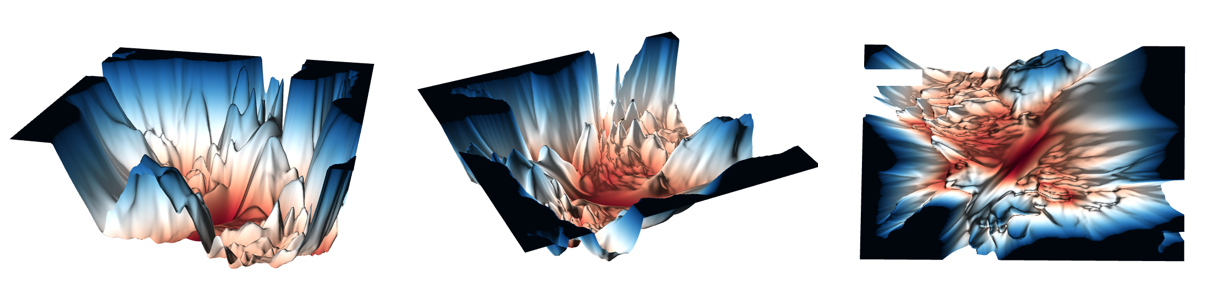
\includegraphics[width=\textwidth]{figures/0intro/intro_landscape.png}
    \caption{A visualisation of the loss landscape of a ResNet-56 model for image classification.}
    \label{fig:high_dim_resnet}
\end{figure}

A saddle point is where among some dimensions, the second-order derivative of the objective is negative, but along others, it is positive. First-order methods slow down in saddle points since they perceive it as a flat region and do not have information about the curvature of the surrounding landscape. This hinders their convergence to a good solution. 

Higher-order methods, by incorporating this curvature information, can identify the nature of saddle points and navigate away from them more effectively. Despite this, it becomes computationally infeasible to process higher-order information. This is because to obtain higher-order information, we would require at least $O(N^2)$ space for $N$ parameters. The computational cost of obtaining higher-order information becomes prohibitive as $N$ increases, which is the case given our deep learning setting. As a practical example, a ResNet-50 model has $N = 25 \times 10^6$ parameters. If we consider each parameter to be represented by 16-bits, we would require $1.25 \times 10^{15}$ bytes, or $1.25$ terabytes of memory to store the second-order information. This is in stark contrast to the $25$ million bytes, or $25$ megabytes, required for first-order information.

\section{KryBall: the best of both worlds}
\label{sec:kryball_intro}

The challenge is to therefore develop an optimisation algorithm that is computationally tractable and scalable, like first-order methods, but can also navigate complex loss landscapes, particularly by escaping saddle points, like higher-order methods. In this thesis, we propose a new optimisation algorithm, KryBall, that combines the benefits of first-order and higher-order methods. We summarise our approach below.

\begin{enumerate}
  \item We use a \textit{Krylov subspace} to approximate local curvature information as a low-dimensional subspace via efficient Hessian-vector products (HvPs).
  \item We analyse this subspace to understand the dominant geometric features of the local landscape. 
  \item We compute the \textit{Saddle-Free Newton} (SFN) direction as a result \citep{dauphin2014sfn}.
  \item We combine this with first-order information such as the gradient and momentum in a \textit{trust region} framework that uses a quadratic model approximation of the local landscape to get a combined, final search direction.
  \item We perform the optimisation step with this direction to optimise our objective.
  \item Optionally, we embed KryBall as a hybrid approach with first-order optimisers such as SGD and Adam, allowing it to be cycled through.
\end{enumerate}

KryBall makes more informed steps than pure first-order methods, particularly in regions like saddle points, while remaining computationally tractable for deep learning. To motivate our method, we show an example in \cref{fig:toy_example}, where first-order methods such as Adam and SGD are hindered on a classic 2D horse saddle, but KryBall successfully escapes it quickly in fewer iterations.

\begin{figure}[h]
  \centering
    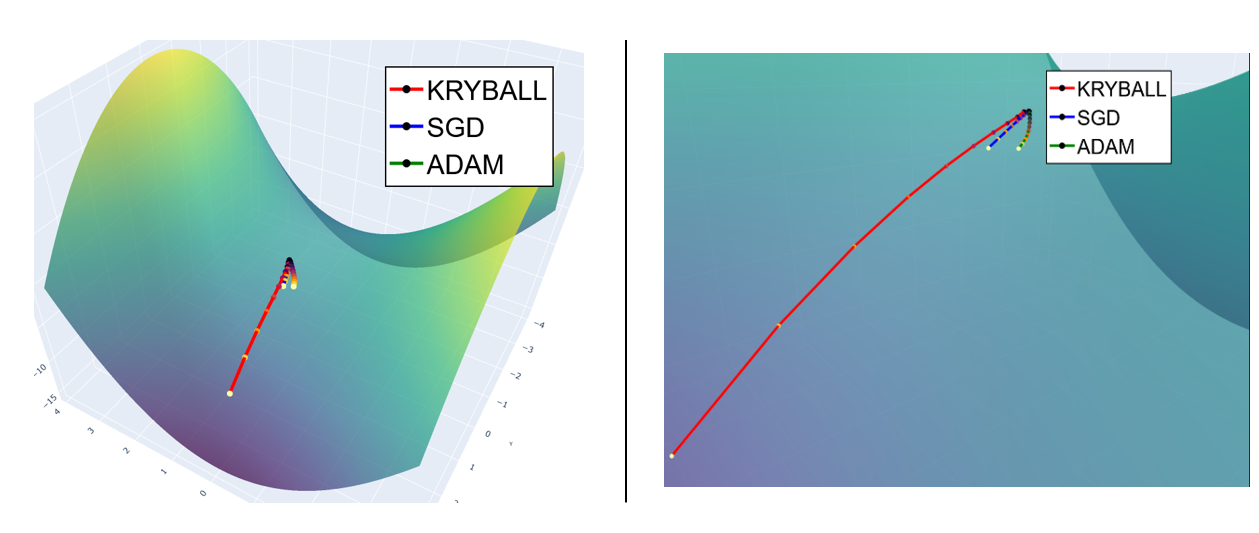
\includegraphics[width=0.85\textwidth]{figures/0intro/intro_toy.png}
    \caption{Left: A classic 2D horse saddle with KryBall, SGD and Adam. Right: A zoomed in version. KryBall successfully escapes the saddle point.}
    \label{fig:toy_example}
\end{figure}

\section{Contributions}
\label{sec:contributions}

Our work focuses on the design and implementation of a novel optimisation algorithm for deep learning, KryBall. In this thesis, we present:
\begin{enumerate}
    \item \textbf{The KryBall Optimisation Algorithm:} The proposal, design, and implementation of KryBall. We combine the benefits of first-order and higher-order methods. KryBall leverages Krylov subspace methods and the SFN direction in a trust-region framework. This enables efficient approximation of local curvature information and navigation of complex loss landscapes, while remaining computationally tractable.
    \item \textbf{Analysis of Loss Landscape Characteristics:} An analysis of the loss landscape properties of common deep learning models and the result of architectural choices (such as activation functions). We investigate the assumptions made when designing an optimiser and the impact of these assumptions on the optimisation process.
    \item \textbf{Extensive Empirical Evaluation:} Experimental validation of KryBall across a range of tasks, such as function optimisation, image classification, and image reconstruction. 
    (\color{red}{can also add the interpretability work here if needs to be more diverse.}\color{black}).
    \item \textbf{A Flexible Experimental Suite:} The development of a modular and configurable software framework for optimiser experiments. This provides a flexible and extensible framework for the implementation, testing, and comparative analysis of various optimisation algorithms. 
    (\color{red}{while not research --- I do think the current framework is a good software suite for a range of tasks that I haven't seen much for optimiser research (except MLPerf). It's quite easy to use, efficient, and extensible. Happy to remove if it doesn't really count as a contribution.}\color{black}).
\end{enumerate}

\section{Thesis outline}
\label{sec:thesis_outline}

To present our contributions, this thesis is organised in the following manner:

\begin{itemize}
    \item \cref{chap:background} provides a mathematical background on optimisation. We formalise the optimisation problem and discuss the geometry of optimisation, including saddle points. This is followed by optimisation in deep learning, where first-order and higher-order methods are explained. We then introduce Krylov subspace methods and trust region algorithms.
    \item \cref{chap:lit_review} provides a comprehensive review of the relevant literature. This includes a survey of first-order and higher-order optimisation algorithms used in deep learning. We compare these methods with our own.
    \item \cref{chap:method} presents the KryBall algorithm. We formally describe its components. This includes the Krylov subspace construction, the SFN computation, and integration with the trust-region framework. We also discuss the assumptions made during the design and outline the hybrid approach.
    \item \cref{chap:results} presents our evaluations. We describe our experimental setup and benchmarking suite. This includes the datasets, model architectures, evaluation metrics, hyperparameter configurations, and comparison with SOTA optimisers. We then present sensitivity analysis and ablation studies.
    \item \cref{chap:discussion} discusses the results. We interpret our findings, analyse potential failure cases and unexpected behaviours, and address current limitations. 
    \item \cref{chap:conclusion} finishes the thesis. We summarise our contributions, discuss the implications of our work, and suggest future work.
\end{itemize}

This chapter has laid the outline for the thesis. We now proceed to \cref{chap:background} to establish the necessary mathematical context.                  % introduction
\chapter{Background}
\label{chap:background}

In this chapter, we provide the relevant technical background required to understand our work. We start by introducing the optimisation problem in \cref{sec:optimisation_problem}. This is continued by a mathematical formulation of the optimisation landscape in \cref{sec:optimisation_landscape}. We then discuss optimisation in deep learning in \cref{sec:optimisation_in_deep_learning}. We end this chapter with a discussion of computationally tractable methods for curvature exploitation in \cref{sec:tractable_curvature_exploitation}.

\section{The Optimisation Problem}
\label{sec:optimisation_problem}

In this section, we formalise the optimisation problem. In the most fundamental case, we minimise an objective function $f$ with respect to real-valued variables with no constraints. The formulation is 
\begin{align}
    \min_{x} f(x)
\end{align}
where
\begin{itemize}
    \item $x \in \mathbb{R}^n$ is a real-valued vector with $n \geq 1$ components,
    \item $f: \mathbb{R}^n \to \mathbb{R}$ is a real-valued function,
    \item $f \in C^k$ s.t. $k \geq 1$ is smooth.
\end{itemize}
We only have a local perspective of $f$, since it is usually expensive to evaluate. We only know what $f$ evaluates to on a limited set of points $x_0, x_1, \ldots, x_k$, in which we use this information to find an optimal point $x^*$ that minimises $f$, as the solution. To do this, we must understand the landscape of $f$ and the scenarios that arise when traversing it.

\section{The Optimisation Landscape}
\label{sec:optimisation_landscape}
In this section, we introduce fundamental concepts that describe the landscape of $f$, which are needed to develop and analyse optimisation algorithms. Here, we introduce the notion of critical points, convexity, and ill-conditioning.

\subsection{Critical Points}
\label{ssec:critical_points}

When exploring the landscape of an objective function, we are interested in identifying specific points of interest that characterise its features. These are called \textit{critical points}. The most desirable of these are \textit{global optima}, in which there are \textit{global minimum} or \textit{global maximum}. An example is provided in \cref{fig:global_min_max}.

\begin{definition}[Global Minimum]
    A point $x^*$ is a \textit{global minimum} if $f(x^*) \leq f(x)$ for all $x$ in the entire domain of $f$.
\end{definition}

\begin{definition}[Global Maximum]
    A point $x^*$ is a \textit{global maximum} if $f(x^*) \geq f(x)$ for all $x$ in the entire domain of $f$.
\end{definition}

\begin{figure}[h]
    \begin{subfigure}[b]{0.48\linewidth}
        \centering
        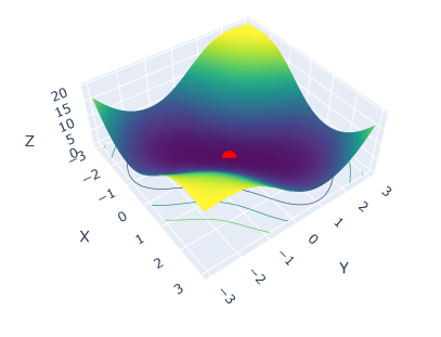
\includegraphics[width=\linewidth]{figures/2background/glob_min.png}
        \caption{A global minimum on \\
        $f(x,y) = (x-\sin(y))^2 + (y-\sin(x))^2$.}
        \label{fig:global_min}
    \end{subfigure}
    \hfill
    \begin{subfigure}[b]{0.48\linewidth}
        \centering
        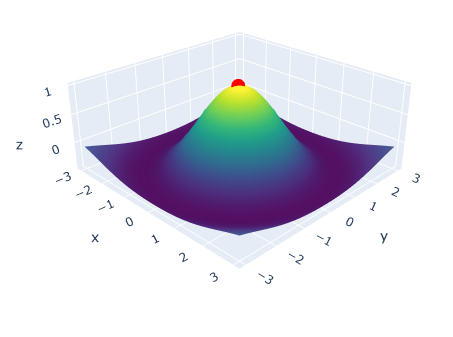
\includegraphics[width=\linewidth]{figures/2background/glob_max.png}
        \caption{A global maximum on \\
        $f(x,y) = \cos(x^2 + y^2) e^{-0.1 (x^2 + y^2)}$.}
        \label{fig:global_max}
    \end{subfigure}
    \caption{Examples of a global minimum and global maximum marked in red.}
    \label{fig:global_min_max}
\end{figure}

Finding such global optima is challenging, as we only have a limited set of information about $f$ and are resource constrained. Thus, many optimisation algorithms aim to find \textit{local optima}, which are points that are locally optimal. Similarly, there are \textit{local minimum} or \textit{local maximum}. We define these points with respect to a neighbourhood $\mathcal{N}$ of a point $x$. We provide examples in \cref{fig:local_min_max}.

\begin{definition}[Local Minimum]
    A point $x^*$ is a \textit{local minimum} if there exists a neighbourhood $\mathcal{N}$ around $x^*$ such that $f(x^*) \leq f(x)$ for all $x \in \mathcal{N}$. It is a \textit{strict local minimum} if instead $f(x^*) < f(x)$ for all $x \in \mathcal{N} \setminus \{x^*\}$.
\end{definition}

\begin{definition}[Local Maximum]
    A point $x^*$ is a \textit{local maximum} if there exists a neighbourhood $\mathcal{N}$ around $x^*$ such that $f(x^*) \geq f(x)$ for all $x \in \mathcal{N}$. It is a \textit{strict local maximum} if instead $f(x^*) > f(x)$ for all $x \in \mathcal{N} \setminus \{x^*\}$.
\end{definition}

\begin{figure}[h]
    \begin{subfigure}[b]{0.48\linewidth}
        \centering
        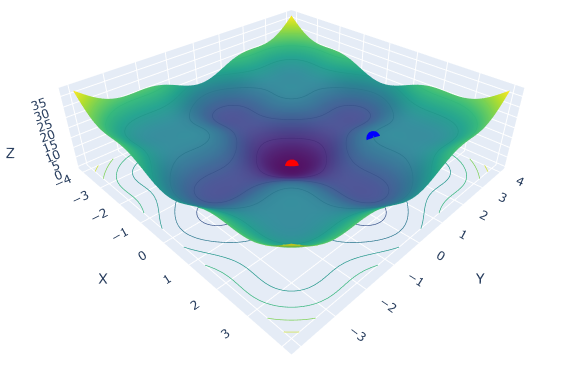
\includegraphics[width=\linewidth]{figures/2background/local_min.png}
        \caption{A local minimum on the egg crate function. \\
        $f(x,y) = (x^2 + y^2) + 5 (\sin(x)^2 + \sin(y)^2)$.
        }
        \label{fig:local_min}
    \end{subfigure}
    \hfill
    \begin{subfigure}[b]{0.48\linewidth}
        \centering
        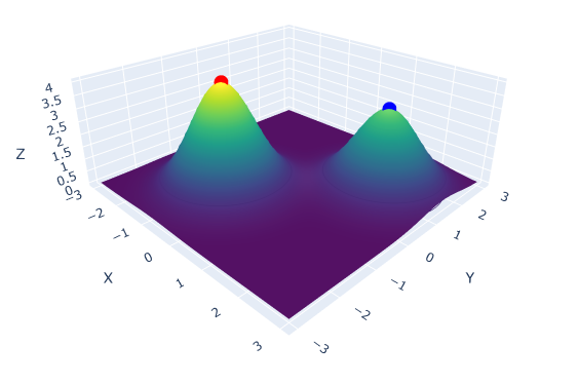
\includegraphics[width=\linewidth]{figures/2background/local_max.png}
        \caption{A local maximum on a multi-bump function. \\
        $f(x,y) = 3 e^{-(x-1.5)^2 - (y-1.5)^2} + \\
         4 e^{-(x+1)^2 - (y+1)^2}$.}
        \label{fig:local_max}
    \end{subfigure}
    \caption{Examples of a local minimum and local maximum marked in blue. The global minimum and global maximum are marked in red for comparison.}
    \label{fig:local_min_max}
\end{figure}

Beyond these, we have \textit{saddle points}. These are points that are locally flat but are neither a local minimum nor a local maximum, as seen in \cref{fig:saddle_point}. In any neighbourhood $\mathcal{N}$ around a saddle point, the function's value increases along some directions emanating from $x^*$ and decreases along others.

\begin{figure}[h]
    \begin{subfigure}[b]{0.48\linewidth}
        \centering
        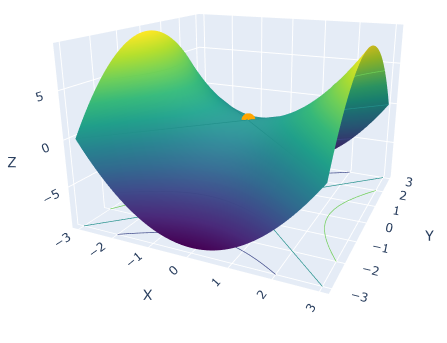
\includegraphics[width=0.8\linewidth]{figures/2background/horse_saddle.png}
        \caption{A saddle point on the horse saddle function. \\
        $f(x,y) = x^2 - y^2$.}
        \label{fig:horse_saddle}
    \end{subfigure}
    \hfill
    \begin{subfigure}[b]{0.48\linewidth}
        \centering
        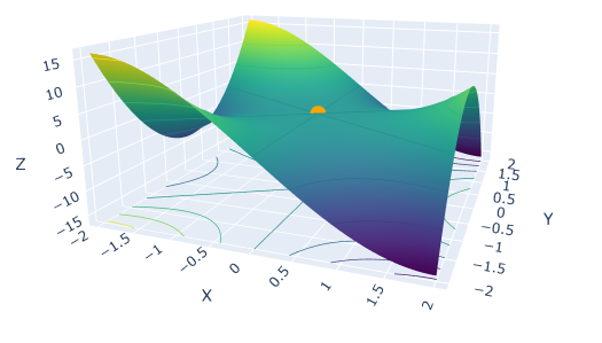
\includegraphics[width=\linewidth]{figures/2background/monkey_saddle.png}
        \caption{A saddle point on the monkey saddle function. \\
        $f(x,y) = x^3 - 3xy^2$.}
        \label{fig:monkey_saddle}
    \end{subfigure}
    \caption{Examples of two functions containing saddle points marked in orange.}
    \label{fig:saddle_point}
\end{figure}

\subsection{Recognising Critical Points}
\label{ssec:recognising_critical_points}

For smooth and differentiable functions, we can recognise critical points using the first and second order information about $f$. Here, we introduce the necessary and sufficient conditions that we can use to do this. We restrict our attention to the class of functions that are twice continuously differentiable, where $f \in C^2$.

We start with a specific type of critical point, a \textit{stationary point}. A key property of any stationary point $x^*$ is that $f$ is locally flat at $x^*$. This implies that its gradient---the vector of \textit{first-order} partial derivatives, $\nabla f(x^*)$---must be zero.
\begin{definition}[Stationary Point]
    A point $x^*$ is a \textit{stationary point} if $f$ is continuously differentiable at $x^*$ and its gradient is zero:
    \begin{align}
        \nabla f(x^*) = 0.
    \end{align}
\end{definition}

Given we are optimising $f$, we want to find a stationary point that is a local minimum. The following definition formalises the \textit{necessary first-order conditions} for a local minimum.
\begin{definition}[Necessary First-Order Conditions]
    If a point $x^*$ is a local minimum, and $f$ is continuously differentiable at $x^*$, then $\nabla f(x^*) = 0$ and $x^*$ is a stationary point.
\end{definition}

We note that all stationary points are critical points, but not all critical points are stationary points. For example, a function may have a critical point at a point where the gradient is undefined. A simple case is when $f(x) = \abs({x})$. This has a critical point at $x = 0$ where the gradient is undefined. However, as mentioned, given we restrict our attention to twice continuously differentiable functions, we do not need to consider these cases. 

All global optima, local optima, and saddle points are stationary points, but not all stationary points are optima. To distinguish between them, we examine the function's local curvature at $x^*$, which is captured by the \textit{Hessian matrix}---an $n \times n$ symmetric matrix of \textit{second-order} partial derivatives of $f$, denoted $\nabla^2 f(x)$ for a point $x$. We abbreviate the Hessian matrix for a function $f$ at a point $x$ as $H$ for convenience. The curvature information captured by $H$ can be summarised by its \textit{eigenvalues}. We denote the $i$-th eigenvalue of $H$, and more generally any symmetric matrix $A$, as $\lambda_i$. We use these eigenvalues to characterise two important properties, \textit{positive semidefiniteness} and \textit{negative semidefiniteness}.

\begin{definition}[Positive Semidefinite Matrix]
    An $n \times n$ symmetric matrix $A$ is \textit{positive semidefinite} if all its eigenvalues are non-negative, where $\lambda_i \geq 0$ for all $i \in [1, n]$.
\end{definition}
\begin{definition}[Negative Semidefinite Matrix]
    An $n \times n$ symmetric matrix $A$ is \textit{negative semidefinite} if all its eigenvalues are non-positive, where $\lambda_i \leq 0$ for all $i \in [1, n]$.
\end{definition}

These properties can now be used to formalise the \textit{necessary second-order conditions} to classify stationary points. We write the necessary second-order conditions for a local minimum as follows.
\begin{definition}[Necessary Second-Order Conditions]
    If a point $x^*$ is a local minimum, and $f$ is twice continuously differentiable, then:
    \begin{itemize}
        \item $\nabla f(x^*) = 0$
        \item $H$ is positive semi-definite.
    \end{itemize}
\end{definition}
Similarly, the above definition can be extended to a local maximum when $H$ is negative semi-definite.

A special case is when $H$ is \textit{indefinite}.
\begin{definition}[Indefinite Matrix]
    An $n \times n$ symmetric matrix $A$ is \textit{indefinite} if it has eigenvalues that are not all positive or negative, where $\exists \lambda_i > 0 \wedge \exists \lambda_j < 0$ for some $i, j \in [1, n]$.
\end{definition}
Here, the function curves upwards in some directions and downwards in others. This is a saddle point.

\begin{definition}[Saddle Point]
    A stationary point $x^*$ is a \textit{saddle point} if $H$ is indefinite.
\end{definition}

Now, we can classify between local minima, local maxima, and saddle points based on whether $H$ is positive/negative semi-definite or indefinite. However, we can still fall short of distinguishing between local minima/maxima and strict local minima/maxima. For example, if $H$ is positive semidefinite, $x^*$ could be a local minimum or a flat region that is not a strict minimum. Similarly, if $H$ is negative semidefinite, $x^*$ could be a local maximum or a flat region. To distinguish between this, we consider two further properties---\textit{positive definiteness} and \textit{negative definiteness}, which are stronger conditions than positive and negative semi-definiteness.

\begin{definition}[Positive Definite Matrix]
    An $n \times n$ symmetric matrix $A$ is \textit{positive definite} if all its eigenvalues are positive, where $\lambda_i > 0$ for all $i \in [1, n]$.
\end{definition}
\begin{definition}[Negative Definite Matrix]
    An $n \times n$ symmetric matrix $A$ is \textit{negative definite} if all its eigenvalues are negative, where $\lambda_i < 0$ for all $i \in [1, n]$.
\end{definition}

We can now guarantee something stricter about the nature of $x^*$, that it is a strict local minimum/maximum. This guarantees that we will optimise our objective without being trapped in a flat region. We write these as the \textit{sufficient second-order conditions} for optimisation. We formalise this for a strict local minimum as follows.
\begin{definition}[Sufficient Second-Order Conditions]
    If $f$ is twice continuously differentiable, and $\nabla f(x^*) = 0$, and $H$ is positive definite at $x^*$, then $x^*$ is a strict local minimum.
\end{definition}
Similarly, we can write the sufficient second-order conditions for a strict local maximum when $H$ is negative definite.

We note that the sufficient second-order conditions are not necessary. A point $x^*$ may satisfy the necessary second-order conditions but fail to satisfy the sufficient second-order conditions. For example, the function $f(x) = x^4$ has a strict local minimum at $x^* = 0$, but $H$ vanishes here and is thus not positive definite at $x^*$. 

\subsection{Convexity}
\label{ssec:convexity}

The property of convexity simplifies the task of finding optima. A function $f$ is \textit{convex} if geometrically, the line segment connecting any two points on the function's graph lies on or above the graph itself. We provide an illustration in \cref{fig:convex_function}, and formally define this as follows.
\begin{definition}[Convex Function]
    A function $f: \mathbb{R}^n \to \mathbb{R}$ is \textit{convex} if its domain is a \textit{convex set}, and for any two points $x_1, x_2$ in its domain, and any scalar $t \in [0, 1]$:
    \begin{align}
        f(t x_1 + (1-t)x_2) \leq t f(x_1) + (1-t)f(x_2).
    \end{align}
    This is a special case of \textit{Jensen's inequality}. Equivalently, a function is convex if $H$ is positive semidefinite for all $x$ in the domain of $f$ given $f$ is twice continuously differentiable.
\end{definition}

\begin{figure}[h]
    \centering
    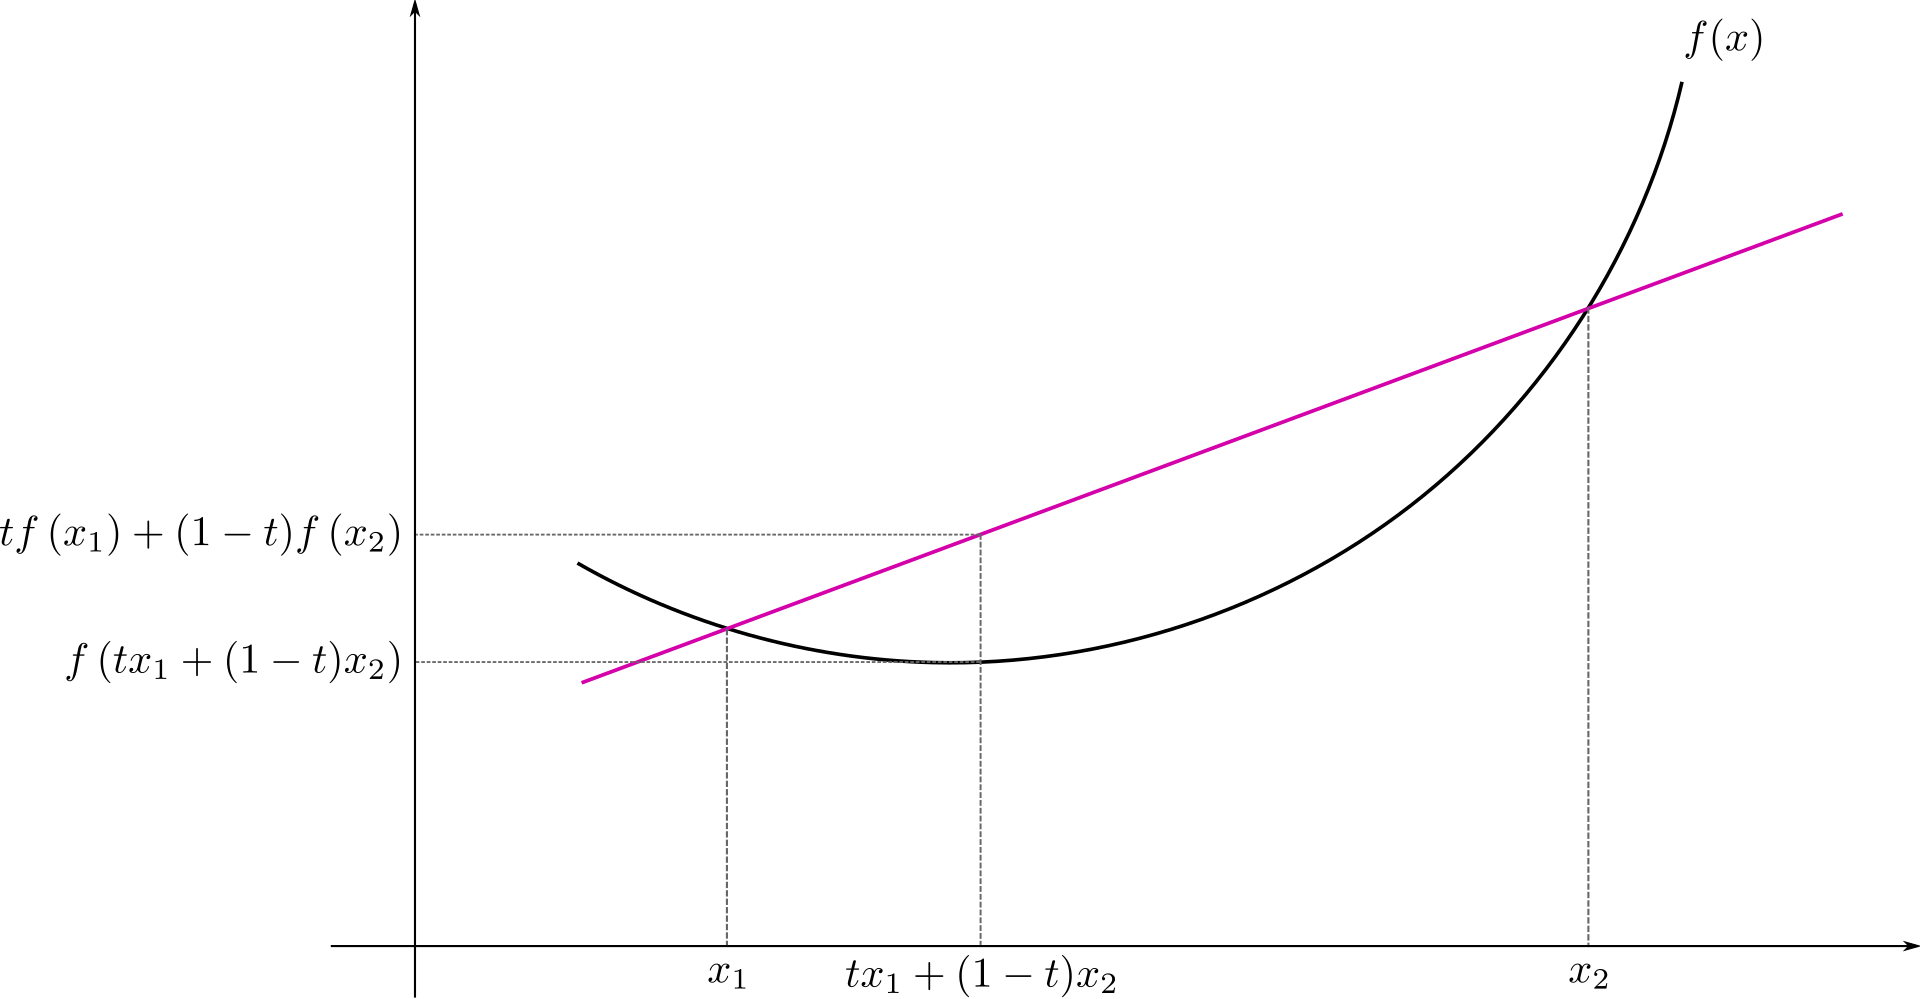
\includegraphics[width=0.7\linewidth]{figures/2background/convex_function.svg.png}
    \caption{An illustration of a convex function. The line segment created by $x_1$ and $x_2$ clearly lies above the function.}
    \label{fig:convex_function}
\end{figure}
Convex functions are particularly appealing because they possess global properties that simplify the optimisation process. We call these properties the \textit{global optimality conditions} for convex functions.
\begin{definition}[Global Optimality Conditions for Convex Functions]
    If $f$ is convex, then: 
    \begin{itemize}
        \item Any local minimum $x^*$ is a global minimum of $f$.
        \item Any stationary point $x^*$ is a global minimum of $f$ given $f$ is continuously differentiable.
    \end{itemize}
\end{definition}

This means that if we find a stationary point of a convex function, we have found the overall best possible solution. Additionally, given that $H$ is guaranteed to be positive semidefinite, certain optimisation algorithms can guarantee convergence to a global minimum regardless of the initialisation point. 

We can further strengthen this by considering the property of \textit{strict convexity}. A strictly convex function is one where the line segment connecting any two points on the function's graph lies strictly above the graph between those points. We illustrate the difference between convex and strictly convex functions in \cref{fig:diff_geometric_convexity}. Formally, we define strictly convex functions as follows.
\begin{definition}[Strictly Convex Function]
    A function $f: \mathbb{R}^n \to \mathbb{R}$ is \textit{strictly convex} if its domain is a convex set, and for any two distinct points $x_1, x_2$ such that $x_1 \neq x_2$ in its domain, and any scalar $t \in (0, 1)$:
    \begin{align}
        f(t x_1 + (1-t)x_2) < t f(x_1) + (1-t)f(x_2).
    \end{align}
    Equivalently, a function is strictly convex if $H$ is positive definite for all $x$ in the domain of $f$ given $f$ is twice continuously differentiable.
\end{definition}

\begin{figure}[h]
    \begin{subfigure}[b]{0.48\linewidth}
        \centering
        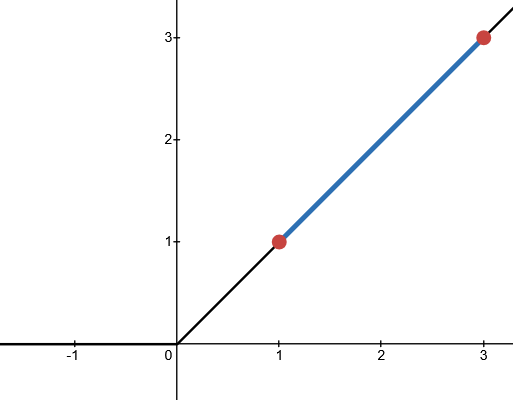
\includegraphics[width=0.8\linewidth]{figures/2background/relu.png}
        \caption{The Rectified Linear Unit (ReLU) function, $f(x) = \max(0, x)$, is convex, but not strictly convex since we can pick two points where the line segment is not strictly above the function.}
        \label{fig:convex_relu}
    \end{subfigure}
    \hfill
    \begin{subfigure}[b]{0.48\linewidth}
        \centering
        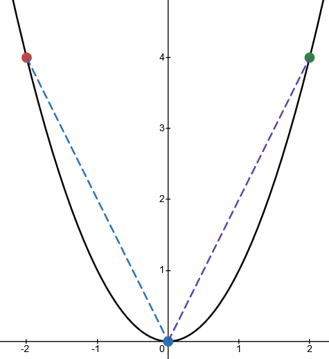
\includegraphics[width=0.6\linewidth]{figures/2background/parabola.png}
        \caption{The parabola function, $f(x) = x^2$, is strictly convex since for any two points, the line segment will always lie above the function.}
        \label{fig:strict_convex_parabola}
    \end{subfigure}
    \caption{The geometrical difference between a convex function and a strictly convex function.}
    \label{fig:diff_geometric_convexity}
\end{figure}


Strictly convex functions are a subset of convex functions. They inherit the same global optimality conditions, but with an additional \textit{uniqueness} property that makes them incredibly easy to optimise.
\begin{definition}[Uniqueness of Global Minimum]
    If $f$ is strictly convex, then there exists \textit{at most one} local minimum of $f$. Consequently, if it exists, then it is the global minimum of $f$.
\end{definition}
Thus, if we find any stationary point of a strictly convex function, we have found the global minimum. This is different from convex functions, where there could be multiple global minima. We provide an illustration of this in \cref{fig:diff_convex_functions}. This makes strictly convex functions incredibly easy to optimise, since we have a guaranteed unique solution.

\begin{figure}[h]
    \begin{subfigure}[b]{0.48\linewidth}
        \centering
        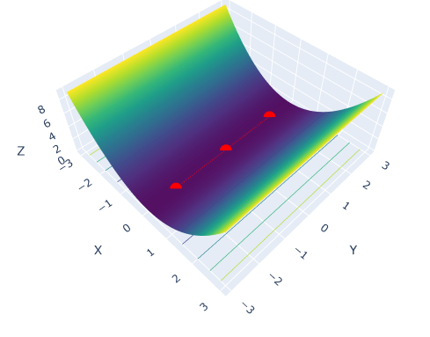
\includegraphics[width=0.8\linewidth]{figures/2background/convex_func.png}
        \caption{Multiple global minima on the convex function
        $f(x,y) = x^2$.}
        \label{fig:convex_func}
    \end{subfigure}
    \hfill
    \begin{subfigure}[b]{0.48\linewidth}
        \centering
        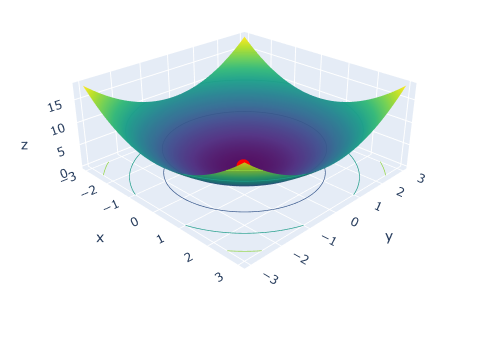
\includegraphics[width=\linewidth]{figures/2background/strict_convex.png}
        \caption{A unique global minimum on the strictly convex function
        $f(x,y) = x^2 + y^2$.}
        \label{fig:strict_convex_func}
    \end{subfigure}
    \caption{The difference between a convex function with multiple global minima and a strictly convex function with a unique global minimum.}
    \label{fig:diff_convex_functions}
\end{figure}


\subsection{Ill-Conditioning and Non-Smoothness}
\label{ssec:ill_conditioning_nonsmooth}

While the nature of critical points and the property of convexity are fundamental to understanding an optimisation problem, other characteristics of the objective function $f$ can also significantly influence the difficulty of finding a solution. We now discuss two such important aspects: ill-conditioning and non-smoothness.

\subsubsection{Ill-Conditioning}
\label{sssec:ill_conditioning}

The \textit{conditioning} of an optimisation problem describes how sensitive the solution $x^*$ is to perturbations in the function $f$ or its parameters. In the context of smooth, twice-differentiable functions, ill-conditioning is primarily associated with the properties of the Hessian matrix $H(x)$ near an optimum. If the eigenvalues of $H(x^*)$ exhibit a wide range of magnitudes, the problem is termed \textit{ill-conditioned}. Geometrically, this often manifests as an objective landscape with long, narrow, and flat valleys leading towards the minimum, or conversely, extremely steep ridges.

A common quantitative measure for ill-conditioning, particularly when $H(x^*)$ is positive definite, is the \textit{condition number}, $\kappa(H)$. It is defined as the ratio of the largest eigenvalue ($\lambda_{max}$) to the smallest eigenvalue ($\lambda_{min}$) of the Hessian:
\begin{align}
    \kappa(H) = \frac{\lambda_{max}}{\lambda_{min}}.
    \label{eq:condition_number}
\end{align}
A large condition number (i.e., $\kappa(H) \gg 1$) signifies a high degree of ill-conditioning. Such landscapes pose considerable challenges for many optimisation algorithms. First-order methods, such as gradient descent, tend to converge very slowly, often exhibiting a characteristic zig-zagging behaviour across the narrow valley instead of proceeding directly towards the minimum. While second-order methods can, in principle, rescale the optimisation space using Hessian information to better navigate ill-conditioned landscapes, the computational burden of accurately forming or approximating and then utilising the Hessian remains a significant hurdle, as previously discussed.

\textbf{TODO: Diagram of ill-conditioned function}

\subsubsection{Non-Smooth Problems}
\label{sssec:non_smooth_problems}

Our discussion has largely presupposed that the objective function $f$ is smooth, typically at least twice continuously differentiable ($f \in C^2$). However, numerous practical optimisation problems, particularly in machine learning, involve \textit{non-smooth functions}. These are functions that may possess points where the gradient, the Hessian, or both, are not well-defined. Such non-smoothness can arise from discontinuities in the function itself or its derivatives. Common examples include functions incorporating absolute values (e.g., $f(x) = |x|$), objectives derived from L1 regularisation which use the L1-norm, or even activation functions like ReLU which have "kinks".

The optimisation of non-smooth functions presents distinct challenges. Standard methods that rely on the existence and computation of gradients (like gradient descent) or Hessians (like Newton's method) may falter or perform erratically because the requisite derivative information is either unavailable or ill-behaved at the points of non-smoothness. The very notion of a unique gradient vector defining a clear direction of steepest descent breaks down.

While a comprehensive exploration of non-smooth optimisation is beyond the purview of this thesis, its prevalence necessitates acknowledgement. Specialised algorithms, such as subgradient methods, bundle methods, and various smoothing techniques, have been developed to address these complexities. In certain specific instances, such as problems involving L1-norm minimisation, it is sometimes possible to reformulate the non-smooth problem into an equivalent smooth, constrained optimisation problem. Nevertheless, for general non-smooth functions, identifying and converging to a minimiser can be considerably more intricate than in the smooth setting.

\section{Optimisation in Deep Learning}
\label{sec:optimisation_in_deep_learning}

% The optimisation principles discussed earlier are key, but applying them in deep learning brings unique challenges. Deep neural networks have vast parameter spaces and very complex, non-convex loss landscapes. This section examines these specific challenges and introduces the main classes of algorithms used to navigate them.

% \subsection{Challenges in High-Dimensional Landscapes}
% \label{ssec:dl_challenges}

% The "curse of dimensionality" is especially evident in deep learning. Models can have millions or even billions of parameters, creating very complex loss landscapes. A key result is the increase in \textit{saddle points} rather than poor local minima. Important studies by \citet{dauphin2014sfn} and \citet{choromanska2015loss} showed that for the high-dimensional, non-convex functions common in neural networks, saddle points become exponentially more frequent than local minima as dimension increases. Additionally, many local minima found in deep learning often have loss values close to the global minimum, making saddle points a greater obstacle to training.

% Saddle points are a major challenge for optimisation algorithms:
% \begin{itemize}
%     \item \textbf{First-order methods}, using only gradient information, can slow down greatly or get stuck near saddle points. The gradient magnitude can be very small near a saddle point, making these methods see the region as flat and progress very little. They don't have curvature information to find escape routes.
%     \item \textbf{Classical second-order methods}, like Newton's method, also face difficulties. If the Hessian at a saddle point has negative eigenvalues (showing negative curvature), the Newton step might move away from the saddle (possibly to areas of higher loss if not handled carefully) or even towards it if the gradient aligns with positive curvature directions.
% \end{itemize}
% Successfully handling these saddle points, not just avoiding bad local minima, is therefore key in deep learning optimisation.

% \subsection{First-Order Methods}
% \label{ssec:first_order_methods}

% First-order optimisation methods are widely used in deep learning because they are computationally efficient and scalable. These methods use the first derivative (gradient) of the objective function to find a minimum.

% \subsubsection{Gradient Descent (GD)}
% The simplest first-order algorithm is Gradient Descent (GD). It repeatedly updates parameters $\theta$ against the gradient of the objective function $f(\theta)$:
% \begin{align}
%     \theta_{t+1} = \theta_t - \alpha \nabla f(\theta_t)
%     \label{eq:gd_update}
% \end{align}
% where $\alpha > 0$ is the \textit{learning rate}, a scalar controlling the step size. While simple, computing the full gradient $\nabla f(\theta_t)$ means evaluating the function over the entire training dataset, which is too computationally expensive for the large datasets often used in deep learning.

% \subsubsection{Stochastic Gradient Descent (SGD)}
% To handle GD's computational cost, Stochastic Gradient Descent (SGD) is commonly used. Instead of the full dataset, SGD estimates the gradient using a small, random data sample called a \textit{mini-batch}. If $g_t(\theta_t)$ is this stochastic gradient estimate at iteration $t$, the update is:
% \begin{align}
%     \theta_{t+1} = \theta_t - \alpha g_t(\theta_t)
%     \label{eq:sgd_update}
% \end{align}
% This greatly reduces the cost per iteration. The randomness adds noise to the gradient estimates, which can help the optimiser escape sharp local minima. But this noise can also slow convergence because updates aren't always in the true steepest descent direction. Mini-batch SGD (often just called SGD in deep learning) is standard practice.

% \subsubsection{Momentum}
% To speed up SGD and reduce oscillations from noisy gradients, \textit{momentum} is often used. Inspired by physics, momentum methods build up an average of past gradients and keep moving in that direction. A common update is:
% \begin{align}
%     v_{t+1} &= \beta v_t + (1-\beta) g_t(\theta_t) \label{eq:momentum_velocity} \\
%     \theta_{t+1} &= \theta_t - \alpha v_{t+1} \label{eq:momentum_update}
% \end{align}
% where $v_t$ is the momentum (or velocity) at iteration $t$, and $\beta \in [0,1)$ is the momentum coefficient. Often, $(1-\beta)$ is part of the learning rate for $g_t$, or a different formula like $v_{t+1} = \beta v_t + \alpha g_t(\theta_t)$ is used, followed by $\theta_{t+1} = \theta_t - v_{t+1}$. The main idea is that updates gain momentum in consistent gradient directions and reduce variations from different mini-batches.

% \subsection{Second-Order Methods}
% \label{ssec:second_order_methods}

% Second-order optimisation methods use curvature information from the objective function, usually with the Hessian matrix. This provides a more direct route to the minimum, especially for poorly shaped landscapes.

% \subsubsection{Newton's Method}
% Newton's method forms a second-order Taylor expansion (a quadratic model) of $f$ around the current point $\theta_t$:
% \begin{align}
%     f(\theta_t + p) \approx f(\theta_t) + \nabla f(\theta_t)^T p + \frac{1}{2} p^T H(\theta_t) p
% \end{align}
% where $H(\theta_t) = \nabla^2 f(\theta_t)$ is the Hessian. The next step $p_t$ comes from minimizing this quadratic model, giving the Newton step:
% \begin{align}
%     p_t = -[H(\theta_t)]^{-1} \nabla f(\theta_t)
%     \label{eq:newton_step}
% \end{align}
% Parameters are updated: $\theta_{t+1} = \theta_t + p_t$. Newton's method can converge quickly (quadratically) near a minimum if the Hessian is positive definite. However, it has major drawbacks for deep learning:
% \begin{itemize}
%     \item \textbf{Computational Cost}: Storing the Hessian takes $O(N^2)$ memory, and inverting it takes $O(N^3)$ operations for $N$ parameters. This is not practical for typical neural networks.
%     \item \textbf{Non-Positive Definite Hessian}: If $H(\theta_t)$ is not positive definite (like near saddle points or areas of negative curvature), the Newton step might not reduce the objective value and could even increase it.
% \end{itemize}

% \subsubsection{Saddle-Free Newton (SFN) Method}
% To fix Newton's method's problems with non-positive definite Hessians, especially how it handles saddle points, changes like the Saddle-Free Newton (SFN) approach exist. The main idea is to change the Hessian matrix $H_t$ so the search direction always reduces the objective and can escape saddles. This is often done by changing its eigenvalues, for instance, by taking their absolute values:
% \begin{align}
%     H_t^{SFN} = V |\Lambda| V^T
%     \label{eq:sfn_hessian}
% \end{align}
% where $H_t = V \Lambda V^T$ is the eigendecomposition of the Hessian, and $|\Lambda|$ is a diagonal matrix with the absolute values of the eigenvalues. The update is then:
% \begin{align}
%     p_t = -[H_t^{SFN}]^{-1} \nabla f(\theta_t)
%     \label{eq:sfn_step}
% \end{align}
% This helps the optimiser treat saddle points like minima from the viewpoint of the changed Hessian, making it easier to escape them. Although SFN solves the saddle point issue for Newton-like methods, it still has the high computational costs of creating, decomposing, and inverting an $N \times N$ Hessian matrix if computed directly.

\section{Methods for Tractable Curvature Exploitation}
\label{sec:tractable_curvature_exploitation}

% While second-order methods like Newton's method offer the promise of rapid convergence by leveraging curvature information, their direct application in deep learning is often crippled by the prohibitive computational cost of forming, storing, and inverting the Hessian matrix. This section introduces techniques that aim to harness curvature information in a more computationally feasible manner.

% \subsection{Krylov Subspace Methods}
% \label{ssec:krylov_methods}

% Krylov subspace methods provide a powerful framework for approximating the solutions to large linear systems or eigenvalue problems without explicitly forming the matrices involved. In the context of optimisation, particularly for approximating the Newton step $p_t = -[H(\theta_t)]^{-1} \nabla f(\theta_t)$, these methods allow us to work with a much smaller, carefully chosen subspace of the full parameter space.

% Given an $N \times N$ matrix $A$ (in our case, often the Hessian $H$) and a vector $v$ (often the gradient $g = \nabla f(\theta_t)$ or the negative gradient), the $m$-th Krylov subspace, denoted $\mathcal{K}_m(A, v)$, is defined as the span of the vectors $\{v, Av, A^2v, \ldots, A^{m-1}v\}$:
% \begin{align}
%     \mathcal{K}_m(A, v) = \text{span}\{v, Av, A^2v, \ldots, A^{m-1}v\}
%     \label{eq:krylov_subspace_definition}
% \end{align}
% Typically, $m \ll N$. The intuition is that this subspace contains rich information about the action of $A$ on $v$. Instead of solving the full $N$-dimensional Newton system $H p = -g$, one can seek an approximate solution $p_m$ that lies within this $m$-dimensional Krylov subspace. This effectively reduces the problem to solving a much smaller system.

% The key to the computational efficiency of Krylov subspace methods is that the basis vectors $v, Av, \ldots, A^{m-1}v$ can be generated iteratively through repeated \textit{matrix-vector products} (in our context, Hessian-vector products, or HvPs, of the form $Hw$ for some vector $w$). Crucially, these HvPs can often be computed efficiently without explicitly forming the full Hessian matrix $H$. Techniques such as automatic differentiation (as used in backpropagation) can be extended to calculate HvPs at a cost that is only a small constant factor more than computing the gradient itself.

% By restricting the search for a direction to a low-dimensional Krylov subspace, these methods can capture dominant curvature information and produce effective Newton-like steps or approximations thereof, while avoiding the $O(N^2)$ storage and $O(N^3)$ computation associated with the explicit Hessian. Algorithms like the Conjugate Gradient (CG) method, a prominent Krylov subspace method, iteratively build up such a subspace to solve linear systems like the Newton equations.
                    % background
\chapter{Literature Review}
\label{chap:lit_review}

% Categorisation/grouping of the literature
% For each cluster, have a section, covers the major academic works thoroughly
%% Describe, advantages/disadvantages including assumptions, major findings, some analysis
%% Compare to self
% Give the impression that you understand the field thoroughly

The work in this thesis is heavily inspired by the advances in deep learning optimisation. In this chapter, we explore the major academic works that have played a significant role in the field of optimisation. In \cref{sec:first_order_methods}, we provide an overview of
first-order methods and their categorisations. This is followed by a discussion of second-order methods and their categorisations in \cref{sec:second_order_methods}. We then look at other techniques in the field, namely non-smooth optimisation and meta-learning in \cref{sec:non_smooth_optimisation} and \cref{sec:meta_learning_discovery}. Following the discussion of each group of works in these respective sections, we will compare and contrast them to our own contributions at the end of the section, which are detailed in the next chapter.

\section{First-Order Methods}
\label{sec:first_order_methods}

In the previous chapter, we saw that an optimisation algorithm in deep learning finds a set of model parameters $\theta^*$ that minimises the loss function $L(\theta)$ introduced in \cref{eq:loss_function}. We covered in \cref{ssec:first_order_methods} that first-order methods are characterised by computing the first order $\nabla_{\theta}L$, or $g$, to use in optimisation. We now look at the different types of first-order methods, including \textit{gradient-based} methods, \textit{momentum} methods, and \textit{adaptive} methods.

\subsection{Gradient-Based Methods}
\label{ssec:gradient_based_methods}

\textbf{Gradient Descent}: One of the earliest methods deployed to solve such optimisation problems is gradient descent (GD). We introduced the concept of steepest descent in \cref{ssec:first_order_methods}, where we saw the parameters being iteratively updated with a scalar multiple, the learning rate $\alpha_{t}$, of the steepest descent direction, the negative gradient $-g$ at each step given an iteration $t$. This gives $\theta_{t+1} = \theta_{t} - \alpha_{t} g_{t}$. Recall that the learning rate $\alpha$ controls the step size of each iteration \citep{ruder2016overview}. GD gradually approaches a local optimum of our loss function $L$, and given appropriate $\alpha$, reaches this sub-linearly if the loss function is \textit{convex}, converging linearly if it is \textit{strongly convex} \citep{NoceWrig06}. However, GD is expensive. In many machine learning tasks, the loss function is evaluated with $N$ samples, each with dimensionality $D$. Thus, GD requires $O(ND)$ per iteration to evaluate. This becomes infeasible very quickly as $N$ and $D$ scale, and disallows online updates and limits model adaptability \citep{ruder2016overview}. While some parallelisation methods were proposed to combat this, the scalability issue still remains \citep{alspector1992parallel,NoceWrig06}. 

\textbf{Stochastic Gradient Descent}: To address the limitations of GD, stochastic gradient descent (SGD) was proposed. Instead of evaluating $g$ using all $N$, a random sample $n \in N$ is picked and instead a stochastic gradient $\hat{g}$, an unbiased estimate of the real gradient, is computed to update $\theta$ \citep{robbins1951stochastic}. SGD achieves the same convergence rates as GD given $L$ satisfies the same convexity conditions \citep{johnson2013accelerating, nemirovski2009robust}. Each iteration reduces from $O(ND)$ to $O(D)$ given only one sample is used.
This overcomes the disadvantage of GD in two ways: online updates can be performed, and convergence can be accelerated, as an optimal $\theta$ can be found using $n << N$ samples \citep{johnson2013accelerating, nemirovski2009robust}. However, the stochastic gradients used in SGD are inherently noisy and fluctuate. These fluctuations can be beneficial, as they allow SGD to jump from one place to another. This behavior is particularly useful in high-dimensional spaces, where we introduced in \cref{ssec:dl_challenges} that most local minima are approximately equal to global minima. If SGD gets trapped in regions such as saddle points where it is hard to make progress, the fluctuations can help escape them.


On the other hand, these fluctuations can also lead to large variance in the gradient estimates \citep{sun2019survey}. This can make the optimisation process unstable and slow convergence. Convergence is also affected by the learning rate $\alpha$. Setting a too low $\alpha$ will slow convergence, and setting a too high $\alpha$ can hinder convergence all together, either overshooting or oscillating at the minimum. Choosing a good $\alpha$ usually requires manual tuning, which is arduous and compute heavy.

\textbf{Mini-batch Stochastic Gradient Descent}: The compromise between SGD and GD resulted in mini-batch stochastic gradient descent (mini-batch SGD) \citep{robbins1951stochastic}. mini-batch SGD splits the $N$ samples into $m << N$ i.i.d \textit{batches} (usually ranging from 64 to 256). $\theta$ is updated each iteration by with the stochastic batch gradient based off one batch. Over time, all batches are processed. This reduces the variance in the gradients and makes convergence more stable, which helps optimisation speed, though we note that the $\alpha$ parameter is still needed. mini-batch SGD is now a mainstream technique used for optimising machine learning models. To align with the standard in the literature, we will refer to mini-batch SGD as SGD from now on.

Our work is different from pure gradient-based methods such as GD and SGD. In particular, our work does not only use the gradient direction, but incorporates this with second-order information. Our step direction is instead a linear combination of the gradient direction with other useful directions minimised in a trust-region framework. Our work also does not need a learning rate like these methods, as we calculate the coefficients from our trust-region framework. However, our work is similar to SGD in that we sample a mini-batch for each iteration to compute the relevant information.

\subsection{Momentum Methods} 
\label{ssec:momentum}

\textbf{Momentum SGD}: Many works have been proposed to improve upon SGD, one of which is momentum (MSGD) \citep{polyak1964some}. The momentum method augments SGD with a \textit{momentum} variable $z$, a decaying average of past gradients controlled by a \textit{momentum factor} $\beta$ \citep{polyak1964some, henriques2019small}. The update is then performed using $z$ as,
\begin{align}
    z_{t+1} &= \beta z_{t} - g_t \\
    \theta_{t+1} &= \theta_t + \alpha z_{t+1}.
\end{align}
This encourages progress along consistent, but small gradient directions. 
MSGD can converge faster, remains more stable under changing $\alpha$, and is more resistant if our loss function is poorly scaled. However, this adds another hyperparameter to tune, and the same problems as seen with $\alpha$ arise. Setting a $\beta$ too low will not result in improvements, and setting it too high can result in overshooting.

\textbf{Nesterov Accelerated SGD}: A small improvement over MSGD is Nesterov-Accelerated SGD (NAG). NAG first updates $\theta$ with $z$, and then calculates the gradient based on the updated $\theta$ \citep{nesterov1983method, sutskever2013importance},
\begin{align}
    \Tilde{\theta}_{t} &= \theta_{t} + \beta z_{t} \\
    z_{t+1} &= \beta z_t - \nabla_{\theta} F(\Tilde{\theta}_{t}) \\
    \theta_{t+1} &= \theta_{t} + \alpha z_{t+1}.
\end{align}
Updating based on the future position of $\theta$ includes more gradient information in comparison to traditional momentum, which can provide a better direction \citep{nesterov1983method, dozat2016nadam}. NAG can also result in superlinear convergence when there is no stochasticity \citep{nesterov1983method, sutskever2013importance}.

Our work incorporates momentum, but it is different from pure momentum-based methods since we also incorporate second-order information. Additionally to emphasise again, we do not need a learning rate like these methods. Our work uses second-order information to complement the momentum and the gradient in a trust-region framework. As such, our work has the benefit of momentum methods, while also having faster convergence from the guarantees of second-order methods. 

\subsection{Adaptive Methods}
\label{ssec:adaptive_methods}

\textbf{AdaGrad}: To tackle the problem of setting an appropriate $\alpha$, adaptive methods that adjust or scale $\alpha$ directly per parameter were proposed \cite{duchi2011adagrad}. The AdaGrad algorithm keeps a history of previous gradients and adjusts the learning rate dynamically \citep{duchi2011adagrad}. It accumulates the historical gradients via squaring, then scales the current gradient \citep{duchi2011adagrad},
\begin{align}
    V_t &= \sqrt{\sum_{i=1}^{t} g_i \odot g_i} \\
    \theta_{t+1} &= \theta_{t} + \alpha \frac{g_t}{V_t + \epsilon},
\end{align}
where $\odot$ denotes element-wise multiplication and the division is also performed element-wise. Note that the $\epsilon$ term is added for numerical stability. The result of this is that only an initial $\alpha$ needs to be set, as during each update the learning rate will adapt due to scaling. Though, as $t \rightarrow \infty$, $V_{t} \rightarrow \infty$, and the learning rate is driven towards zero as the denominator in the update term becomes very large \citep{ruder2016overview,rmsprop2012,zeiler2012adadelta}. This makes the parameter updates ineffective. This is especially the case in non-convex settings and regions such as saddle points, as the learning rate will be very quickly driven to zero before making sufficient progress.

\textbf{RMSProp and AdaDelta}: To address this, instead of accumulating all of the gradients, RMSProp takes inspiration from momentum \citep{ruder2016overview, rmsprop2012}. It uses an exponential decaying moving average to weight the past squared gradients using a decay parameter $p$ \citep{rmsprop2012, kingma2014adam}. The update rule is then,
\begin{align}
    V_t &= \sqrt{p V_{t-1} + (1 - p)g_t^2}.
\end{align}
This simulates having a window size $w$, where gradients outside of this window are forgotten \citep{rmsprop2012, kingma2014adam}. It priorities more recent gradients and so the learning rate is more stable and does not diminish with time. AdaDelta improves upon this and also keeps track of the change in updates, $\Delta(\theta_t)$, performed \citep{zeiler2012adadelta}. This results in
\begin{align}
    U_t = \sqrt{p U_{t-1} + (1 - p)(\Delta(\theta_t))^2}.
\end{align}
AdaDelta then uses these accumulative updates at each iteration to perform the actual update which is 
\begin{align}
    \theta_{t+1} = \theta_{t} - \frac{U_{t-1}}{V_{t} + \epsilon} g_t.
\end{align}
The key observation here is the absence of $\alpha$. This is a step up from most SGD methods, which require the $\alpha$ parameter. The algorithm is also suitable in non-convex settings since there is no diminishing learning rate \citep{zeiler2012adadelta}. However, the absence of $\alpha$ is replaced with $p$ and $\epsilon$ which still need to be tuned, though these are much less sensitive.

\textbf{Adam}: Perhaps the most successful algorithm for optimisation is Adaptive Moment Estimation (Adam) \citep{kingma2014adam}. Adam maintains two moving averages: one for the gradients themselves, $m_t$, and the same $V_t$ used in RMSProp/AdaDelta \citep{kingma2014adam}. Each of these have an associated decay term $\beta_1$ and $\beta_2$, which weight the gradients and the history \citep{kingma2014adam}.
\begin{align}
m_t &= \beta_1 m_{t-1} + (1 - \beta_1) g_t \label{eq:m_t} \\
V_t &= \sqrt{\beta_2 V_{t-1} + (1 - \beta_2) g_t^2} \\
\hat{m_t} &= \frac{m_t}{1 - {\beta_1}^t} \\
\hat{V_t} &= \frac{V_t}{1 - {\beta_2}^t} \\
\theta_{t+1} &= \theta_t - \alpha \frac{\hat{m_t}}{{\hat{V_t}} + \epsilon} \label{eq:adam_update}
\end{align}
We call $m_t$ and $V_t$ the \textit{first} and \textit{second} moment estimates respectively, with $\beta_1$ and $\beta_2$ being the first and second moment hyper-parameters \citep{kingma2014adam}. Adam has a few key advantages. It uses momentum and exponential decay to smooth out gradients, which makes the optimisation process more stable. It also has bias correction applied to $\hat{m_t}$ and $\hat{V_t}$ to allow for proper initialisation \citep{kingma2014adam}. This ensures they are not biased towards their starting estimates. This is important during early stages of optimisation, as there is insufficient data to estimate the moments. Adam is stable and effective in practice, and works well with both convex and non-convex loss functions. Adam is the current SOTA optimisation method in deep learning. However, it lacks theoretical guarantees and convergence is not well understood \citep{reddi2019asmgrad}. Adam has been shown to fail in simple one dimensional convex settings \citep{reddi2019asmgrad}. It additionally needs two extra parameters, $\beta_1$ and $\beta_2$, in comparison to traditional SGD, which need to be tuned.

Our work is similar in concept to these adaptive methods. However, while these methods adjust the learning rates based on historical gradient information, we instead use a trust-region framework. The step sizes are determined by trust-region optimisation. We use second-order information, and do not need a learning rate, or first and second moment hyperparameters. We also have convergence guarantees. However, we note that our work functions as a hybrid with these methods as well. Our work can incorporate the first and second moments into our trust-region to find a step direction, in which we can then incorporate these adaptive learning rates with second-order information. 

\subsection{Adam Variants}
\label{ssec:adam_variants}

\textbf{AdaMax}: Several variants have been proposed to address Adam's limitations. The first variant is AdaMax. AdaMax replaces the $L_2$ norm in $V_t$ with the $L_{\infty}$ norm \citep{kingma2014adam}. Specifically, instead of maintaining the average of the squared gradients $V_t$, AdaMax keeps track of the maximum absolute value of the past gradients \citep{kingma2014adam}.
\begin{align}
    u_t &= \max(\beta_2 \cdot u_{t-1}, |g_t|) \\ 
    \hat{m_t} &= \frac{m_t}{1 - \beta_1^t} \\
    \theta_{t+1} &= \theta_t - \alpha \cdot \frac{\hat{m_t}}{u_t}
\end{align}, 
where we do a component wise max and component wise division. Here, the second moment estimate $\hat{V_t}$ is replaced with $u_t$. This is done to make the algorithm more robust, as $u_1, u_2, \dots, u_t$ are influenced by fewer gradients and thus there is less noise. This is especially the case for when the gradients are large and can become numerically unstable \citep{kingma2014adam}. Note that no bias correction is also needed for $u_t$.

\textbf{NAdam}: Another variant of Adam is Nesterov Adam (NAdam), which extends Adam with the NAG method seen in \cref{ssec:momentum} \citep{dozat2016nadam}. NAdam uses the NAG update by performing the \textit{Nesterov} trick - in which the previous first moment is replaced with the currently calculated first moment similar to NAG \citep{nesterov1983method,dozat2016nadam}. Condensing the Adam update equations from \cref{eq:m_t} to \cref{eq:adam_update} in \cref{eq:nadam_normal}, the following update is changed from 
\begin{align}
    \theta_{t+1} = \theta_t - \frac{\alpha}{{\hat{V_t}} + \epsilon} \left( \beta_1 \mathbf{\hat{m}_{t-1}} + \frac{(1 - \beta_1)g_t}{1 - (\beta_1)^t} \right) \label{eq:nadam_normal}
\end{align}
to 
\begin{align}
    \theta_{t+1} = \theta_t - \frac{\alpha}{{\hat{V_t}} + \epsilon} \left( \beta_1 \mathbf{\hat{m}_{t}} + \frac{(1 - \beta_1)g_t}{1 - (\beta_1)^t} \right).
\end{align}
Like NAG, NAdam uses the future position of $\theta$ to calculate the gradient and incorporate more information in the update. NAdam has been shown to yield sizeable improvements in performance in comparison to Adam on MNIST and Word2Vec tasks \citep{dozat2016nadam}.

\textbf{AdamW}: Decoupled weight decay regularisation, or AdamW, is a further variant of Adam \citep{loshchilov2017decoupled}. Normally, applying L2 regularisation in Adam involves appending the regularisation term to the gradient update as follows,
\begin{align}
    g_t &= \nabla_{\theta} F(\theta_t) + \lambda \theta_{t-1}.
\end{align}
However, upon rescaling, the effect of the regularisation is not properly accounted for and large $g_t$ do not get regularised as much as they should \citep{loshchilov2017decoupled}. To address this, AdamW decouples the weight decay and applies it alongside the update.
\begin{align}
    \theta_{t+1} = \theta_t - \alpha \left( \frac{\hat{m_t}}{\hat{V_t} + \epsilon} + \lambda \theta_t \right).
\end{align}
This is because in adaptive gradient methods, L2 regularisation in the gradient update is \textit{not} the same as weight decay - unlike SGD \citep{loshchilov2017decoupled}. Adam is not effective with L2 regularisation, and so AdamW substantially benefits from this decoupling, improving in performance on CIFAR10 and ImageNet-32 tasks \citep{loshchilov2017decoupled}. AdamW is widely used in practice and is also a current SOTA optimisation method.

\textbf{AMSGrad}: A particularly well-known issue with Adam is the lack of convergence guarantees. One limitation is that in certain scenarios, Adam aggressively increases the learning rate, even when the algorithm is close to the optimum \citep{reddi2019asmgrad}. This is because the second moment term $V_t$ can grow indefinitely, and there is a very high dependence on $\beta_2$. For particular $\beta_2$, highly suboptimal solutions can be reached in the case of simple convex settings \citep{reddi2019asmgrad}.

AMSGrad modifies this by keeping a bound on $\hat{V_t}$ by taking the maximum for the update rule \citep{reddi2019asmgrad}.
\begin{align}
    \hat{V_{t}} &= \max(\hat{V}_{t-1}, V_t)
\end{align}
This guarantees that the learning rate is not increased indefinitely, as each $V_t$ is guaranteed to be non decreasing and at least as large as the previous $V_t$'s \citep{reddi2019asmgrad}. By ensuring this, drastic and aggressive learning rate increases are prevented, and the algorithm convergences better and is more stable. However, AMSGrad is still dependent on $\beta_2$, and cannot show convergence guarantees on any arbitrary $\beta_2$ \citep{taniguchi2024adopt}. Some works have demonstrated that problem dependent tuning of $\beta_2$ can lead to convergence, but this still requires manual tuning \citep{taniguchi2024adopt}.

\textbf{ADOPT}: To address the dependency of convergence on $\beta_2$, ADaptive Gradient Method with the OPTimal Convergence Rate (ADOPT) was most recently proposed \citep{taniguchi2024adopt}. ADOPT shows that by modifying the update rules of Adam, convergence can be attained for any $\beta_2 \in [0, 1]$. The non-convergence of Adam can be attributed to the $V_t$ needing to be conditionally independent of the current gradient $g_t$ \citep{taniguchi2024adopt}. In a normal Adam update as in \cref{eq:adam_update}, the conditional independence criteria is not satisfied. This is because $\hat{V}_t$ contains information about $g_t$, and so convergence breaks. 
ADOPT fixes this by modifying the order of the update and the normalisation \citep{taniguchi2024adopt}. Specifically, the normalisation is applied to the current gradient in a modified update rule of $m_t$, 
\begin{align}
    m_t = \beta_1 m_{t-1} + (1 - \beta_1) \frac{g_t}{\hat{V}_{t-1} + \epsilon^2}.
\end{align}
Here, the previous second moment, $V_{t-1}$ is used to ensure this conditional independence with $g_t$ when scaling and so convergence is guaranteed. In practice, ADOPT uses $\max(\hat{V}_{t-1}, \epsilon)$ instead of $\hat{V}_{t-1} + \epsilon^2$ for the normalisation for performance benefits \citep{taniguchi2024adopt}. The parameter update is shortly applied after as
\begin{align}
    \theta_{t+1} = \theta_{t} - \alpha \cdot m_{t+1}.
\end{align}
ADOPT outperforms Adam, AdamW, and AMSGrad on MNIST and CIFAR10 image classification tasks \citep{taniguchi2024adopt}.
It achieves substantial improvements in LLM pretraining and finetuning tasks over Adam and the rest of the variants as well \citep{taniguchi2024adopt}. 

Our work presents a different paradigm from these Adam variants. While these variants focus on the convergence and reliance on tuning, as we mentioned in the previous section, our work does not need explicit learning rate and moment hyperparameters. Our work has theoretical convergence guarantees due to our trust-region framework, whereas these works address the problem of Adam's convergence rather than exhibiting these guarantees. However, as mentioned previously, we do note that our work can work as a hybrid with these variants, as we can incorporate all of this information into our trust-region framework.

\section{Second-Order Methods}
\label{sec:second_order_methods}

As discussed in \cref{chap:background}, first-order methods are effective for many optimisation problems, but fall short when the optimisation landscape is ill-conditioned or challenging. We saw that second-order methods address these problems in \cref{ssec:second_order_methods}, as they find or approximate the Hessian $H$. We now discuss the different types of second order methods. 

\subsection{Newton and Quasi-Newton Methods} 
\label{sec:newton_methods}

\textbf{Damped and Regularised Newton Methods}:
We saw in \cref{ssec:second_order_methods} that while Newton's method offers rapid quadratic convergence, it may not produce a descent direction, when the Hessian $H$ is not positive definite or when far from a solution. Damped and regularised Newton methods improve the robustness and global convergence properties of the standard Newton step. One approach is \textit{step-size damping}. This method introduces the learning rate $\alpha_t \in (0, 1]$ to scale the Newton direction, similar to first-order methods we saw in \cref{sec:first_order_methods} \citep{sun2019survey}:
\begin{align}
    \theta_{t+1} = \theta_t - \alpha_t H_t^{-1} g_t.
\end{align}
The step length $\alpha_t$ is typically chosen using a line search at each iteration to ensure sufficient decrease. This prevents overly aggressive steps and improves stability. Another approach is \textit{regularisation damping}. Instead of scaling the step, this method modifies the Hessian matrix $H_t$ directly to ensure it is sufficiently positive definite. A common technique is to add a constant $\lambda$ to the eigenvalues of $H_t$ before inversion. This yields the update:
\begin{align}
    H_t &= V^T \Lambda V \\
    B_t &= (V^T (\Lambda + \lambda I) V)^{-1} \\
    \theta_{t+1} &= \theta_t - B_t g_t.
\end{align}
This damps the eigenvalues of $H_t$, ensuring the modified Hessian is well-conditioned. The parameter $\lambda_t$ can be adjusted adaptively,and instead of adding, we can scale the eigenvalues of $H_t$. As we noted in \cref{ssec:trust_region_methods}, this formulation is closer to the solution of the trust-region subproblem. Both damping strategies enhance the reliability of Newton's method, making it more applicable to the non-convex landscapes. However, we note that the computational cost is still a problem. With regularisation damping, we need to explicitly perform an eigendecomposition of $H_t$ and then reconstruct our modified Hessian. This is intractable for large $H_t$ as the eigendecomposition is $O(N^3)$. Thus, while these methods increase the stability of Newton's method while maintaining the convergence properties, the computation intractability still remains.

\textbf{BFGS}: We address the computational infeasibility of Newton methods with Quasi-Newton methods. Quasi-Newton methods compute an explicit approximation of the Hessian, rather than computing it directly. The Broyden-Fletcher-Goldfarb-Shanno (BFGS) algorithm generates a sequence of matrices to estimate the Hessian \citep{NoceWrig06}. It iteratively refines the estimate using gradient information and rank-two updates at each iteration \citep{NoceWrig06}. The estimate is always positive-definite. Through experimental testing and analysis, these estimates are quite good. BFGS also has effective self-correcting properties. If an estimate becomes poor at one iteration, within the next few it will correct itself \citep{NoceWrig06}. BFGS reduces the complexity to $O(N^2)$ for computation time \citep{NoceWrig06, sun2019survey}.  

A common variant of BFGS, Limited BFGS (L-BFGS), reduces the memory requirement by storing $k$ vectors instead of retaining the full $n\times n$ approximations \citep{NoceWrig06, sun2019survey}.

\textbf{SR1}: The Symmetric Rank-One (SR1) method further tackles the infeasibility problem. It approximates the inverse Hessian using the difference between a history of gradients and positions, while ensuring symmetry in the update \citep{NoceWrig06}. The key advantage of SR1 is that it uses only rank-updates, but also does not guarantee positive definiteness \citep{NoceWrig06}. This makes it beneficial in non-convex settings, where positive definiteness guarantee is hard to maintain. Albeit at the cost of stability, it helps the algorithm capture more curvature information.

\textbf{Stochastic Quasi-Newton with Trust Region}: BFGS and SR1 methods can be adapted into a stochastic setting with a trust-region framework. sL-BFGS-TR and sL-SR1-TR were proposed as methods following this setting. These methods compute the Hessian approximation $D_t$ at each iteration using either L-BFGS or SR1. This $D_t$ is then used in the second-order approximation of $L$ to solve the trust-region subproblem. Results for sL-BFGS-TR and sL-SR1-TR show that they are efficient and are able to keep up with Adam on MNIST and CIFAR10 tasks \citep{yousefi2023deep}. Specifically, as batch size increases, these algorithms are faster than Adam on models such as LeNet, ResNet and a 3C3L (3 Convolution 3 Linear) ConvNet \citep{yousefi2023deep}. Together with an effective mini-batch sampling strategy, sL-BFGS-TR and sL-SR1-TR converge faster than Adam \citep{yousefi2023deep}. This shows that Quasi-Newton methods can be effective in deep learning, and can be used in a stochastic setting, even if contrary to popular belief.

Our work differs from traditional Quasi-Newton methods like BFGS, L-BFGS, and SR1 in its approach to curvature information. Our work instead directly utilises HVPs to build an approximation instead of using rank-one or rank-two updates. Our work also incorporates momentum and the gradient in a trust-region framework to get our step direction, instead of relying purely on the second-order approximation. Additionally, while the sL-BFGS-TR and sL-SR1-TR methods use a trust-region, our approach is different. We use subspace optimisation to solve the trust-region subproblem and to find a linear combination of useful directions, whereas these methods instead use other methods to solve the subproblem and instead maintain an explicit Hessian approximation matrix. 

\subsection{Diagonal Hessian Estimation} 
\label{ssec:diag_hessian}

\textbf{AdaHessian}: As Quasi-Newton methods aim to estimate the inverse Hessian, improvements have been made to use diagonal hessian estimates as well. AdaHessian modifies the second moment from Adam to use the squared diagonal estimate of the Hessian \citep{yao2021adahessian}.
\begin{align}
    \hat{D}_t &\approx \text{diag}(H_t) \\
    V_t &= \sqrt{\beta_2 V_{t-1} + (1 - \beta_2) \hat{D}_t\hat{D}_t}
\end{align}
This brings down the space complexity to $O(D)$, and makes it more feasible to use incorporate second order information \citep{yao2021adahessian}. Though, as a trade-off, an extra backward pass is required per iteration. AdaHessian performs well in image classification, NLP, and recommender system tasks \citep{yao2021adahessian}.

\textbf{Sophia}: A more effective approach to using diagonal estimates was proposed by Second-order Clipped Stochastic Optimisation (Sophia) \citep{liu2023sophia}. Sophia uses a diagonal estimate of the Hessian as a preconditioner to the first moment in the update rule alongside a clipping mechanism. This was motivated by heterogenous curvature in deep learning models, in which traditional optimisers struggle with \citep{liu2023sophia}. 

Sophia first computes the diagonal estimate of the Hessian, $\bar{D}_t$, every $k$ iterations using either the Hutchinson or Gauss-Newton-Bartlett estimation methods via an estimator $E$ \citep{liu2023sophia}. 
\begin{align}
    \hat{D}_t &= E(H_t) \quad E \in \{\text{Hutchinson, Gauss-Newton-Bartlett} \} \\
    \bar{D}_t &= 
    \begin{cases}
        \beta_2 \bar{D}_{t-k} + (1 - \beta_2) \hat{D}_t & \text{if } t \mod k = 1, \\
        \bar{D}_{t-1} & \text{otherwise}
    \end{cases}
\end{align}
This is then put into a clipping function that controls the worst case size update, in which the update rule is
\begin{align}
    \theta_{t+1} = \theta_t - \alpha \cdot \text{clip}(\frac{m_t}{\max(\gamma \cdot \bar{D}_t, \epsilon)}, \rho)
\end{align}
where $\text{clip}(z, p) = \max(\min(z, p), -p)$ and $\gamma$, $\rho$ are hyper-parameters that function as a scaling factor and a clipping threshold respectively \citep{liu2023sophia}. We saw in \cref{ssec:second_order_methods} that incorporating second-order information through the Newton step can result in moving in the wrong direction. To counter this, Sophia considers only the positive entries of $\bar{D}_t$, and clips each coordinate to a maximum step size of $p$ (where $p = 1$ usually) \citep{liu2023sophia}. If any entry of $\bar{D}_t$ is negative, Sophia falls back to momentum signSGD. This is a method in which the update is scaled by the sign of the gradient for each component, ignoring the magnitude. This ensures that in the worst case, the update is controlled with a size of $p$, improving stability. On language modelling tasks, Sophia converges quicker and achieves better performance in comparison to AdamW \cite{liu2023sophia}.

Our work is different since it utilises curvature information from Hessian-vector products, instead of relying on diagonal Hessian estimates. 
However, our work is similar in that we use a clipping threshold to clip the eigenvalues of our Hessian approximation. We also can optionally use diagonal estimates to precondition the vector used for the HVPs when building our approximation. Our work is more stable than Sophia, as it offers a richer representation of the local curvature. We also use a trust-region framework which these works do not employ. 

\subsection{HVP-based Methods}
\label{ssec:hvp_based_methods}

\textbf{Hessian-Free Optimisation}: Hessian-free optimisation (HF) uses HVPs to incorporate second-order information \citep{NoceWrig06, martens2010hessianfree}. Similar to Newton's method, a search direction is computed by solving the following linear system, where $\alpha_t$ is a step size computed to guarantee sufficient decrease \citep{martens2010hessianfree}.
\begin{align}
    H_t d_t &= - g_t \\
    \theta_{t+1} &= \theta_t - \alpha_t d_t.
    \label{equation:hessian_free_lin_sys}
\end{align}
The system in \cref{equation:hessian_free_lin_sys} is solved with the conjugate-gradient solver (CG), an iterative method that solves linear systems. This computes the HVP without using the Hessian, which reduces the space to $O(N)$ and results in $O(KN)$ time, where $K << N$ controls the number of iterations used for CG \citep{martens2010hessianfree}. However, the CG solver can be very unstable when $H_t$ is not positive definite. Thus, it breaks down when dealing with noise and stochasticity. Ill-conditioned and non-convex problems also add to these issues.

\textbf{CurveBall}: Combining fast HVP's and curvature information with the heavy-ball framework was introduced with CurveBall, hence it's name. CurveBall uses a quadratic approximation like the Newton method, and solves the optimisation problem by solving the same linear system as in \cref{equation:hessian_free_lin_sys}. Instead of using CG or matrix inversion, it uses GD to optimise on $d_t$ and finds $\Delta d_t$ \cite{henriques2019small}. 
\begin{align}
    \Delta d_{t+1} &= H_t d_t + g_t \\
    z_{t+1} &= \beta z_{t} - \alpha_2 \Delta d_{t+1} \\
    \theta_{t+1} &\leftarrow \theta_t + \alpha_1 z_{t+1}
\end{align}
The advantage to this is that there is no restriction on $H$. The algorithm can work in non-convex and ill-conditioned problems too, as demonstrated by it's performance on Rosenbrock and the Rahimi-Recht function \citep{henriques2019small}. The $\Delta d_{t}$ variable keeps track of how $H_t$ and $g_t$ change as $\theta$ evolves, which incorporates the curvature. To amortize cost, it interleaves updates between $\theta$ and $\Delta d_{t+1}$ \citep{henriques2019small}. With the use of fast HVP's through forward-mode (FMAD) and backward-mode automatic differentiation (RMAD), it requires only two passes of back-propagation \citep{henriques2019small}, as we discussed in \cref{ssec:hessian_vector_products}. This makes it highly efficient and scalable, in which it demonstrates better performance on MNIST and CIFAR10 classification tasks \citep{henriques2019small}.  

Our method is similar to these works since the core of it is using HVPs. However, we do not use CG or GD to optimise and solve the linear system present in \cref{equation:hf_lin_sys}. The problem we solve is similar, but not the same as \cref{equation:hf_lin_sys}, as ours is a regularised/damped version of it. We also solve this problem in a low dimensional subspace generated through Krylov subspaces, and then compute useful search directions from this and embed them in a trust-region framework.

\subsection{Subspace Optimisation Methods}
\label{ssec:subspace_opt_methods}

\textbf{Krylov Subspace Descent}: Approximate solutions to optimisation problems in low dimensional subspaces are also a popular strategy to involve curvature information. Krylov Subspace Descent (KSD) constructs a basis of vectors $\mathcal{K}_m$ and then finds a search direction in $\mathcal{K}_m$ using BFGS \citep{vinyals2012krylov}. The Krylov basis is constructed with diagonal Hessian estimate preconditioning \citep{vinyals2012krylov}.
\begin{align}
    \mathcal{K}_m = \{(D^{-1}H)^{k}D^{-1}g | \quad 0 \leq k \leq m \}
\end{align}
During optimisation, this subspace is converted into a new non-orthogonal subspace $\hat{\mathcal{K}_m}$, where BFGS is run to find to ${\hat{K}v}$ as the search direction, where $\hat{K} \in \hat{\mathcal{K}_m}$ \citep{vinyals2012krylov}. KSD exhibits lower training error and faster running time in comparison to HF on MNIST \citep{vinyals2012krylov}. It also has no assumptions on $H$, unlike HF which has stability issues if $H$ is not positive semidefinite.

Our method is quite similar to Krylov Subspace Descent. Both approaches construct a low-dimensional subspace using HVPs. However, the subsequent utilisation of this subspace differs. KSD applies an optimiser like BFGS within the generated Krylov subspace to find a search direction. In contrast, our method instead embeds search directions found within this subspace alongside the gradient and the momentum in a trust-region. We thus derive our update from the trust-region rather than directly optimising within the initial Krylov subspace.  

\section{Non-smooth Optimisation}
\label{sec:non_smooth_optimisation}

For some problems, there may be conditions on the loss function such that it is non-smooth and that $g$ is intractable to calculate. We now look at optimisation methods that address this case.

\textbf{Coordinate Descent}: Coordinate Descent (CD) aims to perform one dimensional search across along each axis direction of $\theta$, till all directions are chosen properly to find optimal $\theta$. Naively, a set of bases $E = {e_1, ..., e_D }$ are chosen where $D = \dim(\theta)$. The parameter space is broken down into individual dimensions or coordinates, and optimization proceeds along each direction sequentially \citep{conn2009derivfree}. As such, the update at the $j$th dimension is given by
\begin{align}
    \theta^{t+1}_j = \arg\min_{\theta_j \in \mathbb{R}} L(\theta^{t+1}_1, \dots, \theta^{t+1}_{j-1}, \theta_j, \theta^t_{j+1}, \dots, \theta^t_D).
\end{align}
This guarantees convergence, as $L$ is set to decrease or stay the same at each iteration, and the convergence of CD is similar to that of GD \citep{conn2009derivfree}. The main difference to GD is that each update is always axis aligned, whereas the $g$ in GD may not be aligned with any $e \in E$. Given the algorithm focuses on one dimension at a time, the update is simple, even for complex problems. It is useful for in settings where there is low $D$ or sparse structures. While highly impractical for deep learning settings, as $D$ is high and we are not given the sparsity structure, setting a coordinate basis may be beneficial to accelerate convergence.

\section{Meta-Learning Discovery}
\label{sec:meta_learning_discovery}

A new way to solve optimisation problems is to consider abstracting away the problem. Meta-learning discovery aim to formulate algorithm search such that optimisation methods are found as a result.

\textbf{Lion}: Evo\textbf{L}ved S\textbf{i}gn M\textbf{o}me\textbf{n}tum (Lion) was discovered via a meta-learning approach \citep{chen2024symbolic}. It uses momentum and the sign operation to update parameters.
\begin{align}
    \text{update} &= \text{sign}(\beta_1 m_{t-1} + (1 - \beta_1)g_t) \\ 
    \theta_{t+1} &= \theta_t - \alpha \cdot \text{update} \\ 
    m_t &= \beta_2 m_{t-1} + (1 - \beta_2)g_t
\end{align}
Unlike adaptive methods, there is no second moment $V_t$, and so no normalisation on the first moment is performed. Thus, Lion contributes a fixed size update to $\theta$ at each iteration, only scaling by the output of the $\text{sign}$ function. This is similar to signSGD, mentioned in \cref{ssec:diag_hessian} under Sophia. Lion is advantageous given that it is simple and only tracks the momentum. This halves the memory requirement, making it more efficient. Lion gains up to a 2.3x speedup on AdamW \citep{chen2024symbolic}. It outperforms AdamW on image classification, vision-language contrastive learning, diffusion modelling and language modelling and pre-training tasks \citep{chen2024symbolic}. However, we note that this is the case only on transformer models that Lion is very effective. Further evaluations proving Lion's effectiveness on non-transformer based models are needed to confirm its effectiveness.

Our method is different entirely from the paradigm of meta-learning since we do not formulate optimisation as an algorithm search. Our method is similar to Lion since we use momentum, but we do not perform a signed update. We also do not use a learning rate or momentum hyperparameters, as previously mentioned. We use HVPs and a trust-region to approximate the local curvature, and our update step is a combination of the momentum, gradient, and other useful directions.                      % lit review
\chapter{The KryBall Optimisation Algorithm}
\label{chap:method}

In this chapter, we present the KryBall optimisation algorithm. We first present the components of the algorithm, including the Krylov subspace construction, the SFN computation, and integration with the trust-region framework. We then discuss the hybrid approach used in KryBall.

                        % method 
\chapter{Evaluation and Analysis}
\label{chap:evaluation}

In this chapter, we present our evaluation, findings, and analysis of our method, the KryBall optimisation algorithm. We start by discussing the implementation of KryBall in \ref{sec:implementation}. We then present the experimental setup in \ref{sec:experimental_setup}, which includes the datasets, models, metrics, hyperparameter settings, and tasks to be evaluated. This is followed by our results in \ref{sec:results}, where we include our empirical evaluations and sensitivity analysis. We then interpret our findings and do some further analysis in \ref{sec:discussion_and_further_analysis}. Finally, we discuss the limitations of our method in \ref{sec:limitations}.

\section{Implementation}
\label{sec:implementation}

Most machine learning workflows and tasks are implemented entirely in Python, and leverage the PyTorch library \citep{pytorch}. This is because PyTorch has efficient low-level kernels and bindings that allow for automatic differentation and tensor operations \citep{pytorch}. We design our optimiser to be integrated seamlessly with PyTorch. As such, KryBall can act as a drop-in replacement for other PyTorch optimisers in deep learning tasks.

\subsection{Adhering to the PyTorch Optimiser API}
\label{ssec:adhering_to_the_pytorch_optimiser_api}

Our implementation adheres to the PyTorch optimiser API while simplifying the standard training workflow. In a typical training setup in PyTorch, users must explicitly call the following functions \citep{pytorch}:
\begin{itemize}
    \item \verb|.backward()| to create the computation graph and the associated gradients.
    \item \verb|.zero_grad()| to clear previous gradients.
    \item \verb|.step()| to perform the optimisation step and update the model parameters.
\end{itemize}
We instead consolidate these into just a single \verb|step| function. This makes it cleaner than the current workflow while maintaining full compatibility with the PyTorch ecosystem. This results in a more clean implementation for end users that reduces boilerplate code. 

In addition, we provide an interpretable way to track necessary information. In PyTorch, optimiser parameters such as momentum and adaptive learning rates are associated with individual parameter blocks and buried within the optimiser's internal state dictionaries \citep{pytorch}. This makes it difficult to understand how they behave during training. Our implementation exposes these quantities directly as accessible vectors, allowing researchers to easily inspect gradients, momentum terms, and other optimisation variables. This facilitates deeper insights into the optimisation process and enables more effective understanding and debugging.

\subsection{Function Integration with PyTorch}
\label{ssec:function_integration_with_pytorch}

% Nit: Cite the github repos
We also introduce a novel test suite that integrates classic functions (Rosenbrock, 2D Saddle, Monkey Saddle etc.) with PyTorch. Currently, most existing implementations that offer direct optimisation of just functions do not integrate with PyTorch. Instead, they all use numerical solvers and approximate the first and second-order derivatives. This is because PyTorch workflows are primarily for deep learning, and simple function optimisation is not a focus. To our knowledge, there exists only a few libraries that try and integrate function optimisation with deep learning. However, these are outdated, lack maintainability, and do not use modern PyTorch techniques such as model JIT compilation to improve speed. We thus implement an easy way to optimise any function with PyTorch optimisers such as SGD, Adam and LBFGS that adheres to the standard training loop. We show an example in \cref{alg:optimise_function_with_pytorch}.

\begin{algorithm}[h]
    \small
    \DontPrintSemicolon
    T = 100\;
    model = Rosenbrock()\;
    optimiser = torch.optim.LBFGS(model.parameters())\;
    \For{$t=1, 2, \ldots, T$}{
        optimiser.zero\_grad()\;
        loss = model()\;
        loss.backward()\;
        optimiser.step()\;
    }
    \caption{Optimising a function with PyTorch optimisers}
    \label{alg:optimise_function_with_pytorch}
\end{algorithm}


\subsection{The Trust-Region Framework}
\label{ssec:the_trust_region_framework}

% Nit: cite this
A core contribution that we present is a novel implementation of $N$-dimensional subspace optimisation that solves the trust-region subproblem. To our knowledge, this is the first general-purpose implementation tailored for deep learning applications within the PyTorch ecosystem. Many trust-region frameworks either employ the dogleg method, or 2D subspace optimisation, but also are not integrated with PyTorch. We thus implement a general-purpose $N$-dimensional subspace optimiser that can be used with any PyTorch optimiser, and more generally any task that involves the trust-region subproblem. 

\subsection{Loss Landscape Sampling}
\label{ssec:loss_landscape_sampling}

The final part of our contributions that we implement is the ability to inspect the loss landscape of deep learning training tasks. We implement a sampler that can be used to sample trajectories from the loss landscape of a deep learning model. Given a particular point in training, our sampler can investigate the local geometry by performing an exhaustive line search along the optimiser's step direction. This allows researchers to visualise and analyse the characteristics of the loss landscape in the vicinity of the optimisation trajectory for a particular optimiser. To our knowledge, this has not been done before, and we use this to analyse the trajectory of optimisers for different deep learning tasks in \cref{sec:discussion_and_further_analysis}. This inspection tool enables deeper insights into optimisation dynamics, and can help explain why certain optimisers perform better on specific tasks, and at which points in training they suffer.

\section{Experimental Setup}
\label{sec:experimental_setup}
% Introduction to this section
To evaluate KryBall, we must first define a diverse range of tasks that accurately reflect the challenges faced by deep learning models. In this section, we define these tasks with respect to the datasets, models, metrics, and hyperparameter tuning setups. We consider the following tasks as our suite: ill-conditioned functions, binary classification, and image classification. Our optimiser suite primarily consists of the MSGD and Adam, which were introduced in \cref{chap:lit_review}, and our KryBall optimiser. 

\subsection{Baselines}
\label{ssec:baselines}
Before we introduce our tasks, we first define our baselines. We select MSGD and Adam as our baseline optimisers. These are state-of-the-art first-order optimisers that we find outcompetes other optimisers in literature. MSGD is a simple and foundational approach that is well-suited for many deep learning tasks. Adam is more of a modern and practical baseline, and has been the standard optimiser in practice ever since it was introduced. We also use LBFGS as a second-order baseline, as it exhibits good performance across many tasks and is also a popular optimiser in practice. However, we note that we only use LBFGS where it is tractable, and so for the image classification task in \cref{ssec:task_3_image_classification}, we do not use LBFGS to remain consistent.

\subsection{Task 1: Ill-Conditioned Function Optimisation}
\label{ssec:task_1_ill_conditioned_function_optimisation}
The first set of tasks involves minimising ill-conditioned objective functions. We choose the Rosenbrock function and implement a noisy, stochastic variant of it, and the Rahimi-Recht function, which we briefly mentioned in \cref{sssec:ill_conditioning} of \cref{chap:background}.

% TODO: Cite properly
\subsubsection{Stochastic Rosenbrock Function}
\label{sssec:task_1_rosenbrock_function}
We implement a stochastic variant of the Rosenbrock function from \cite{henriques2019small}. We have that $\mathcal{R}: \mathbb{R}^2 \rightarrow \mathbb{R}$:
\begin{equation}
\mathcal{R}(x, y) = (1 - x)^2 + 100\epsilon_i(y - x^2)^2,
\end{equation}
where at each evaluation of the function, a noise sample $\epsilon_i$ is drawn from a uniform distribution $\mathcal{U}[\lambda_1, \lambda_2]$ with $\lambda_1 \leq \lambda_2$. When $\lambda_1 = \lambda_2 = 1$, we can recover the deterministic Rosenbrock function with its well-known minimum at $(x, y) = (1, 1)$. To assess robustness to noise, we compare each optimiser on both the deterministic formulation and two stochastic variants with different noise regimes.

% TODO: Cite Henriques and Rahimi and Recht
\subsubsection{Rahimi-Recht Function}
\label{sssec:task_1_rahimi_recht_function}
The second function is an ill-conditioned linear regression problem introduced by Rahimi and Recht \citep{recht2017kitchen}. This involves training a neural network with two linear layers to approximate a linear map with a high condition number. The objective function is
\begin{equation}
\mathcal{L}(W) = \|\hat{y} - y_{true}\|^2 = \|W_L W_{L-1} \cdots W_1 x - Ax\|^2, 
\end{equation}
where $A$ is an ill-conditioned matrix with condition number $\kappa$, and $W_i$ are the weight matrices of the linear network. We construct the true linear map $A_{true} \in \mathbb{R}^{m \times d}$ with singular values linearly spaced between 1 and $\kappa$ \citep{recht2017kitchen}. We generate $n=1000$ random input samples and compute the corresponding outputs using this map. The behaviour of this function is that as we get closer to the minima, it becomes increasingly ill-conditioned. Specifically, the eigenvalues of the Hessian tend towards infinity.

\subsubsection{Evaluation Setup and Metrics}
\label{sssec:task_1_evaluation_setup_and_metrics}
We evaluate MSGD, Adam, LBFGS, and KryBall on the Rosenbrock and the Rahimi-Recht functions with the following chosen ill-conditioning parameters:
\begin{itemize}
    \item \textbf{Deterministic Rosenbrock}: $\lambda_1 = \lambda_2 = 1$.
    \item \textbf{Stochastic Noisy Rosenbrock}: $\lambda_1 = 0$, $\lambda_2 = 1$.
    \item \textbf{Stochastic Noisy Rosenbrock}: $\lambda_1 = 0$, $\lambda_2 = 3$.
    \item \textbf{Slightly Ill-Conditioned Rahimi-Recht}: $\kappa = 10$.
    \item \textbf{Highly Ill-Conditioned Rahimi-Recht}: $\kappa = 1e5$.
\end{itemize}
Each optimiser is tuned using Hyperband on each function for 20 sweeps, where each sweep has 100 epochs. We describe in detail our hyperparameter tuning setup in \cref{ssec:hyperparameter_tuning_setup}. We then use the best performing configuration for each optimiser, and then run all optimisers with a budget of 2000 epochs until they converge within an $\epsilon$ of the solution or use up the computational budget. For Rosenbrock, we choose $\epsilon = 1 \times 10^{-4}$ and for Rahimi-Recht we choose $\epsilon = 1 \times 10^{-2}$. Here, we are measuring the optimisers ability to converge to the solution while handling noise and ill-conditioning.

\subsection{Task 2: XOR Classification}
\label{ssec:task_2_xor_classification}

The next task we consider is a simple case of binary classification with the XOR function. This is a good task to bridge between the ill-conditioned functions and more complex recognition tasks as it introduces non-linearity. The XOR task cannot be linearly separated, and needs a non-linear activation function. Our dataset is simple and small. It includes all 4 combinations of inputs to the XOR function, a 2D vector of zeros and ones, and the corresponding labels in which they evaluate to.

\subsubsection{Evaluation Setup and Metrics}
\label{sssec:task_2_evaluation_setup_and_metrics}
% TODO: Reference BCE
For this task, we use a simple MLP with 3 layers, consisting of one input layer, a hidden layer with a hidden dimension of size 8, and an output layer. Our activation function is the Softplus function, and our loss function is the Binary Cross Entropy (BCE) loss \citep{mao2023cross}. The BCE loss is defined as
\begin{equation}
\mathcal{L}(y, \hat{y}) = -\frac{1}{N} \sum_{i=1}^N \left[ y_i \log \hat{y}_i + (1 - y_i) \log (1 - \hat{y}_i) \right],
\end{equation}
and measures the difference between the predicted probability distribution and the actual distribution which consists of the ground truth labels for a binary classification task \citep{mao2023cross}. This is useful for the XOR case since our output is binary.

We test MSGD, Adam, LBFGS, and KryBall on this task. Each optimiser is tuned for 20 sweeps, each with 100 epochs like the previous task. We use the best performing parameters, and then run each optimiser on the XOR task with a budget of 100 epochs. Given this task is quite simple, and our chosen model is more than capable, we measure the number of epochs it takes to converge. Our convergence criteria here is to reach perfect accuracy, that is an accuracy of 1.0, and completely minimise the loss function (reach 0 loss). This means we have perfectly predicted the XOR problem. In practice, most models and most optimisers are capable of this, and thus we instead focus on convergence speed. 

\subsection{Task 3: Image Classification}
\label{ssec:task_3_image_classification}

Our third and final task is a suite of image classification problems. Here, given an image $I$ that is usually either a binary image or an RGB image, we want to classify it into one of $C$ classes. We thus use a variety of datasets to formulate our image classification problem.

\subsubsection{MNIST-1D}
\label{sssec:task_3_mnist_1d}
MNIST-1D is a scaled down one-dimensional version analogue of the classic MNIST handwritten digit dataset \citep{greydanus_mnist1d}. It consists of 40-dimensional time series signals that represent the handwritten digits from 0 to 9. These are constructed through procedural generation and involve random transformations such as padding, translation and scaling operations \citep{greydanus_mnist1d}. There are 5000 total samples in MNIST-1D, where 4000 are allocated for training and 1000 for testing \citep{greydanus_mnist1d}. Each example in MNIST-1D is labeled with its corresponding digit class (0--9). This estbalishes a 10-class classification problem where the ground truth represents the original digit template from which each signal was derived.

\subsubsection{CIFAR-10}
\label{sssec:task_3_cifar_10}
CIFAR-10 is widely used dataset for image classification. It consists of 60000 RBG images that are of size $32 \times 32 \times 3$ \citep{cifar10}. These are distributed across 10 distinct object classes: irplane, automobile, bird, cat, deer, dog, frog, horse, ship, and truck. The dataset comprises 50000 training images and 10000 test images \citep{cifar10}. Each class contains exactly 6000 images, where the train and test split is 5000 and 1000 respectively. The ground truth for this dataset is a single-label classification that indicates the primary object category present in each image \citep{cifar10}. In CIFAR-10, all images are labelled. We note that a superset of CIFAR-10 is CIFAR-100, which instead contains 100 classes. 

\subsubsection{Evaluation Setup and Metrics}
We evaluate our optimisers on the MNIST-1D and CIFAR-10 datasets. We categorise our experiments into three different groups which are based on the model we use. We now describe each of these groups.

\begin{itemize}
    \item \textbf{MNIST-1D MLP}: We use the simple MLP we had from the XOR task. Here, we modify the hidden dimension to be of size 256. This is consistent with the original implementation for MNIST-1D in \citep{greydanus_mnist1d}, and offers a good baseline for this task.
    \item \textbf{CIFAR-10 CNN}: The first model we use to evaluate on CIFAR-10 is a 3-layer Convolutional Neural Network (CNN) with 2 fully connected layers. Here, we use three convolutional layers with 32, 32 and 64 output channels, each using $5 \times 5$ kernels with padding. Each convolution is followed by batch normalisation, our choice of activation and average pooling. We then follow with two fully connected layers to predict out output.
    \item \textbf{CIFAR-10 ResNet-18}: We also evaluate using a stronger model, a ResNet-18, introduced by \citep{resnet}. This deeper architecture employs residual connections to enable training of networks with 18 layers, where each layer consists of four residual blocks with skip connections. ResNet-18 is a baseline architecture for CIFAR-10, and offers good performance in which we can evaluate our optimisers on. 
\end{itemize}
For each model, we use the Softplus activation as done previously. 

For this image classification task, we employ the Categorical Cross Entropy (CCE) loss function \citep{mao2023cross}. This generalises the BCE loss to multi-class classification problems, extending it to handle $C$ classes \citep{mao2023cross}. This is done by comparing the predicted probability distribution over all classes with the true one-hot encoded label distribution. The CCE loss is defined as
\begin{equation}
\mathcal{L}(y, \hat{y}) = -\frac{1}{N} \sum_{i=1}^N \sum_{c=1}^C y_{i,c} \log \hat{y}_{i,c}.
\end{equation}
Here, $N$ is the number of samples, $C$ is the number of classes, and $y_{i,c}$ is the true label, where it is 1 if sample $i$ belongs to class $c$ or 0 otherwise, and $\hat{y}_{i,c}$ is the predicted probability for sample $i$ belonging to class $c$. CCE measures the difference between the predicted probability distribution and the actual distribution. This makes it well-suited for CIFAR-10 with given its 10 distinct object categories.

Our metrics for this task are the test accuracy and the training loss. Specifically, we look at the peak test accuracy and final test accuracy achieved during training. We also consider the final training. This shows how well our optimiser is able to train these different models on different datasets.

\subsubsection{Training Setup}
\label{sssec:task_3_training_setup}

Our training setup is distinct from other tasks. Here, we sample mini-batches during training since evaluating on the whole dataset is infeasible. This is unlike our previous tasks, which were not highly parameterised. We now detail the batch size and the number of epochs for each task.
\begin{itemize}
    \item \textbf{MNIST-1D MLP}: The batch size is 512 and we train for 100 epochs.
    \item \textbf{CIFAR-10 CNN}: The batch size is 256 and we train for 40 epochs.
    \item \textbf{CIFAR-10 ResNet-18}: The batch size is 128 and we train for 40 epochs.
\end{itemize}

\subsection{Hyperparameter Tuning Setup}
\label{ssec:hyperparameter_tuning_setup}

All of our experiments are tuned with Bayesian hyperparameter search combined with the Hyperband early stopping algorithm \citep{li2018hyperband}. Hyperband is a bandit-based algorithm that allocates resources to promising configurations while eliminating poorly performing ones early in training \citep{li2018hyperband}. We choose a halving factor $\eta = 3$, which eliminates the worst-performing configurations, retaining only the top $\frac{1}{3}$ of candidates at each successive halving round. This significantly reduces computational cost by avoiding full training of suboptimal hyperparameter combinations. We set a minimum iteration threshold of 10 epochs before any configuration can be terminated, ensuring sufficient training time for meaningful performance evaluation.

\begin{itemize}
    \item \textbf{MSGD}: Learning rate $\alpha \in [1 \times 10^{-4}, 1]$ under a log uniform distribution, momentum $\beta \in [0.8, 0.99]$ under a uniform distribution.
    \item \textbf{Adam}: Learning rate $\alpha \in [1 \times 10^{-4}, 1]$ under a log uniform distribution, betas $\beta_1 \in [0.9, 0.999]$ and $\beta_2 \in [0.99, 0.99999]$ under a uniform distribution.
    \item \textbf{LBFGS}: Learning rate $\alpha \in [1 \times 10^{-4}, 1]$ under a log uniform distribution.
    \item \textbf{KryBall}: Krylov subspace size $k \in [1, 10]$ under an integer uniform distribution, krylov refresh rate $r_{\mathit{refresh}} \in [1, 10]$ under an integer uniform distribution.
\end{itemize}

\subsection{Experimental Infrastructure}
\label{ssec:experimental_infrastructure}
We run our evaluations and experiments on a single machine that consists of an NVIDIA RTX 3070 GPU with 8GB VRAM, and a Ryzen 5 3600 CPU with 6 cores, with a clock speed of 3.6 GHZ. We also have 32GB DDR4 memory of available. For our software, we use Python 3.12.4, and PyTorch 2.4.0 on a Linux Subsystem. This is complemented by CUDA version 12.6. We use the Weights and Biases platform to track and run all of our experiments and tune our hyperparameters. We run our experiments with maximum GPU memory usage, and our GPU utilisation was monitored to be around 0.30 in all runs. This is consistent with GPU utilisation rate for mainstream machine learning workloads.    

\section{Results}
\label{sec:results}
In this section, we present our empirical evaluations of KryBall. We present our results and the comparisons of KryBall with other optimisers for each of the tasks we have defined in \cref{ssec:task_1_ill_conditioned_function_optimisation}, \cref{ssec:task_2_xor_classification}, and \cref{ssec:task_3_image_classification}. We then present our sensitivity analysis in \cref{ssec:second_order_methods}. For each task, we discuss the results and analyse our findings. 

\subsection{Task 1: Ill-Conditioned Function Optimisation}
\label{ssec:results_ill_conditioned_function_optimisation}

\Cref{tab:task_1_convergence_table} summarsies our results of optimising ill-conditioned functions. Here, we present the epochs until convergence, where we defined our criteria earlier in \cref{ssec:task_1_ill_conditioned_function_optimisation}. We see in \cref{tab:task_1_convergence_table} that KryBall and LBFGS outclass MSGD and Adam when optimising the Rosenbrock function. Specifically, LBFGS converges the fastest regardless of the Rosenbrock variant. This is followed by KryBall, which is competitive with LBFGS. However, we note that LBFGS represents the \textit{ideal convergence} in practice, since for each iteration it evaluates the function multiple times and backtracks. This is contrast to our method, which only evaluates the function once. Thus, we see that our method is competitive in practice with the ideal case. 

\begin{table}[!t]
    \caption{Epochs until convergence for each optimiser on the Rosenbrock and Rahimi-Recht functions. The best values denote fastest convergence, and are bolded and highlighted in green. Divergence is represented by N/A and highlighted in red.}
    \label{tab:task_1_convergence_table}
    \begin{tabular}{cccccc}
    \hline
    \multicolumn{1}{l}{} & \multicolumn{5}{c}{\textbf{Epochs Until Convergence $\downarrow$}}                                                                                                                                   \\ \hline
                         & \multicolumn{3}{c}{\textbf{Rosenbrock}}                                                                      & \multicolumn{2}{c}{\textbf{Rahimi-Recht}}                                \\
                         & \textbf{$\mathcal{U}[1,1]$}                & \textbf{$\mathcal{U}[0,1]$}                & \textbf{$\mathcal{U}[0,3]$}                & \textbf{$\kappa = 10$}                      & \textbf{$\kappa = 1 \times 10^5$}                      \\ \hline
    \textbf{MSGD}        & 248                                & 624                                & 1587                               & \cellcolor[HTML]{FFFFFF}94         & \cellcolor[HTML]{FD6864}N/A         \\
    \textbf{Adam}        & 249                                & 981                                & 1978                               & 242                                & \cellcolor[HTML]{FFFFFF}1720        \\ \hline
    \textbf{LBFGS}       & \cellcolor[HTML]{34FF34}\textbf{5} & \cellcolor[HTML]{34FF34}\textbf{5} & \cellcolor[HTML]{34FF34}\textbf{5} & \cellcolor[HTML]{34FF34}\textbf{6} & \cellcolor[HTML]{FD6864}N/A         \\
    \textbf{KryBall}     & \cellcolor[HTML]{34FF34}\textbf{5} & 13                                 & 16                                 & 51                                 & \cellcolor[HTML]{34FF34}\textbf{52} \\ \hline
    \end{tabular}
\end{table}

This is further evidenced by the optimiser trajectories for the Rosenbrock variants in \cref{fig:rosenbrock_results}. KryBall and LBFGS are impacted little by the ill-conditioning and are able to converge. LBFGS is able to converge very quickly as it takes very large steps in the optimisation landscape. It also takes a near perfect path, and can correct itself. We see this in \cref{fig:deterministic} as it overshoots the solution, but then re-evaluates and reaches the solution. This is a testament to LBFGS's backtracking and ability to evaluate the function multiple times. Our method also demonsrates this ability, and as it gets closer to the solution takes a path similar to LBFGS.

On the other hand, we see that MSGD and Adam make little progress and can be unstable. In \cref{fig:deterministic}, both MSGD and Adam become unstable when trying to take large steps. In \cref{fig:stochastic_1} and \cref{fig:stochastic_2}, MSGD and Adam make very little progress per iteration. This shows that for ill-conditioned functions, MSGD and Adam are not able to take large steps and remain stable. This supports our hypothesis that ill-conditioned functions are a problem for first-order methods, as we discussed in \cref{chap:background}.

For the Rahimi-Recht function, we see all optimisers being able to reach the minimum when the problem is slightly ill-conditioned. \Cref{fig:rr_losses_k_10} and \cref{fig:rr_losses_k_1e5} show the loss curves for the two instances of the Rahimi-Recht function. Our problem of interest is \cref{fig:rr_losses_k_1e5}, where the function is severely ill-conditioned. We see in \cref{tab:task_1_convergence_table} that only KryBall and Adam are able to converge, while MSGD and LBFGS diverge. Adam converges very slowly and exhibits instability as it approaches the minimum. However, it does not diverge like MSGD. We suspect that Adam's adaptive learning rate is advantageous for highly ill-conditioned functions, as it can adaptively scale each parameter. This is beneficial since, as we approach the minimum, the eigenvalues of the Hessian become increasingly large. MSGD's constant momentum scaling is thus insufficient to handle this eigenvalue spread, which explains why it diverges so rapidly.

We also suspect LBFGS diverges because its limited-memory Hessian approximation becomes increasingly inaccurate when the function is highly ill-conditioned, leading to poor search directions. This is unlike KryBall, which maintains reliable curvature information. This allows our method to adapt the approximation quality and step sizes dynamically, enabling rapid convergence even in these highly ill-conditioned settings.

In summary, our method exhibits rapid convergence. It is competitive with the practical best possible convergence as illustrated by LBFGS. We also exhibit good stability and the ability to handle severe ill-conditioning, and are able to outperform state-of-the-art first-order methods on these problems.

% Nit: SGD should be MSGD 
\begin{figure}[!t]
    \begin{subfigure}[b]{0.49\linewidth}
        \centering
        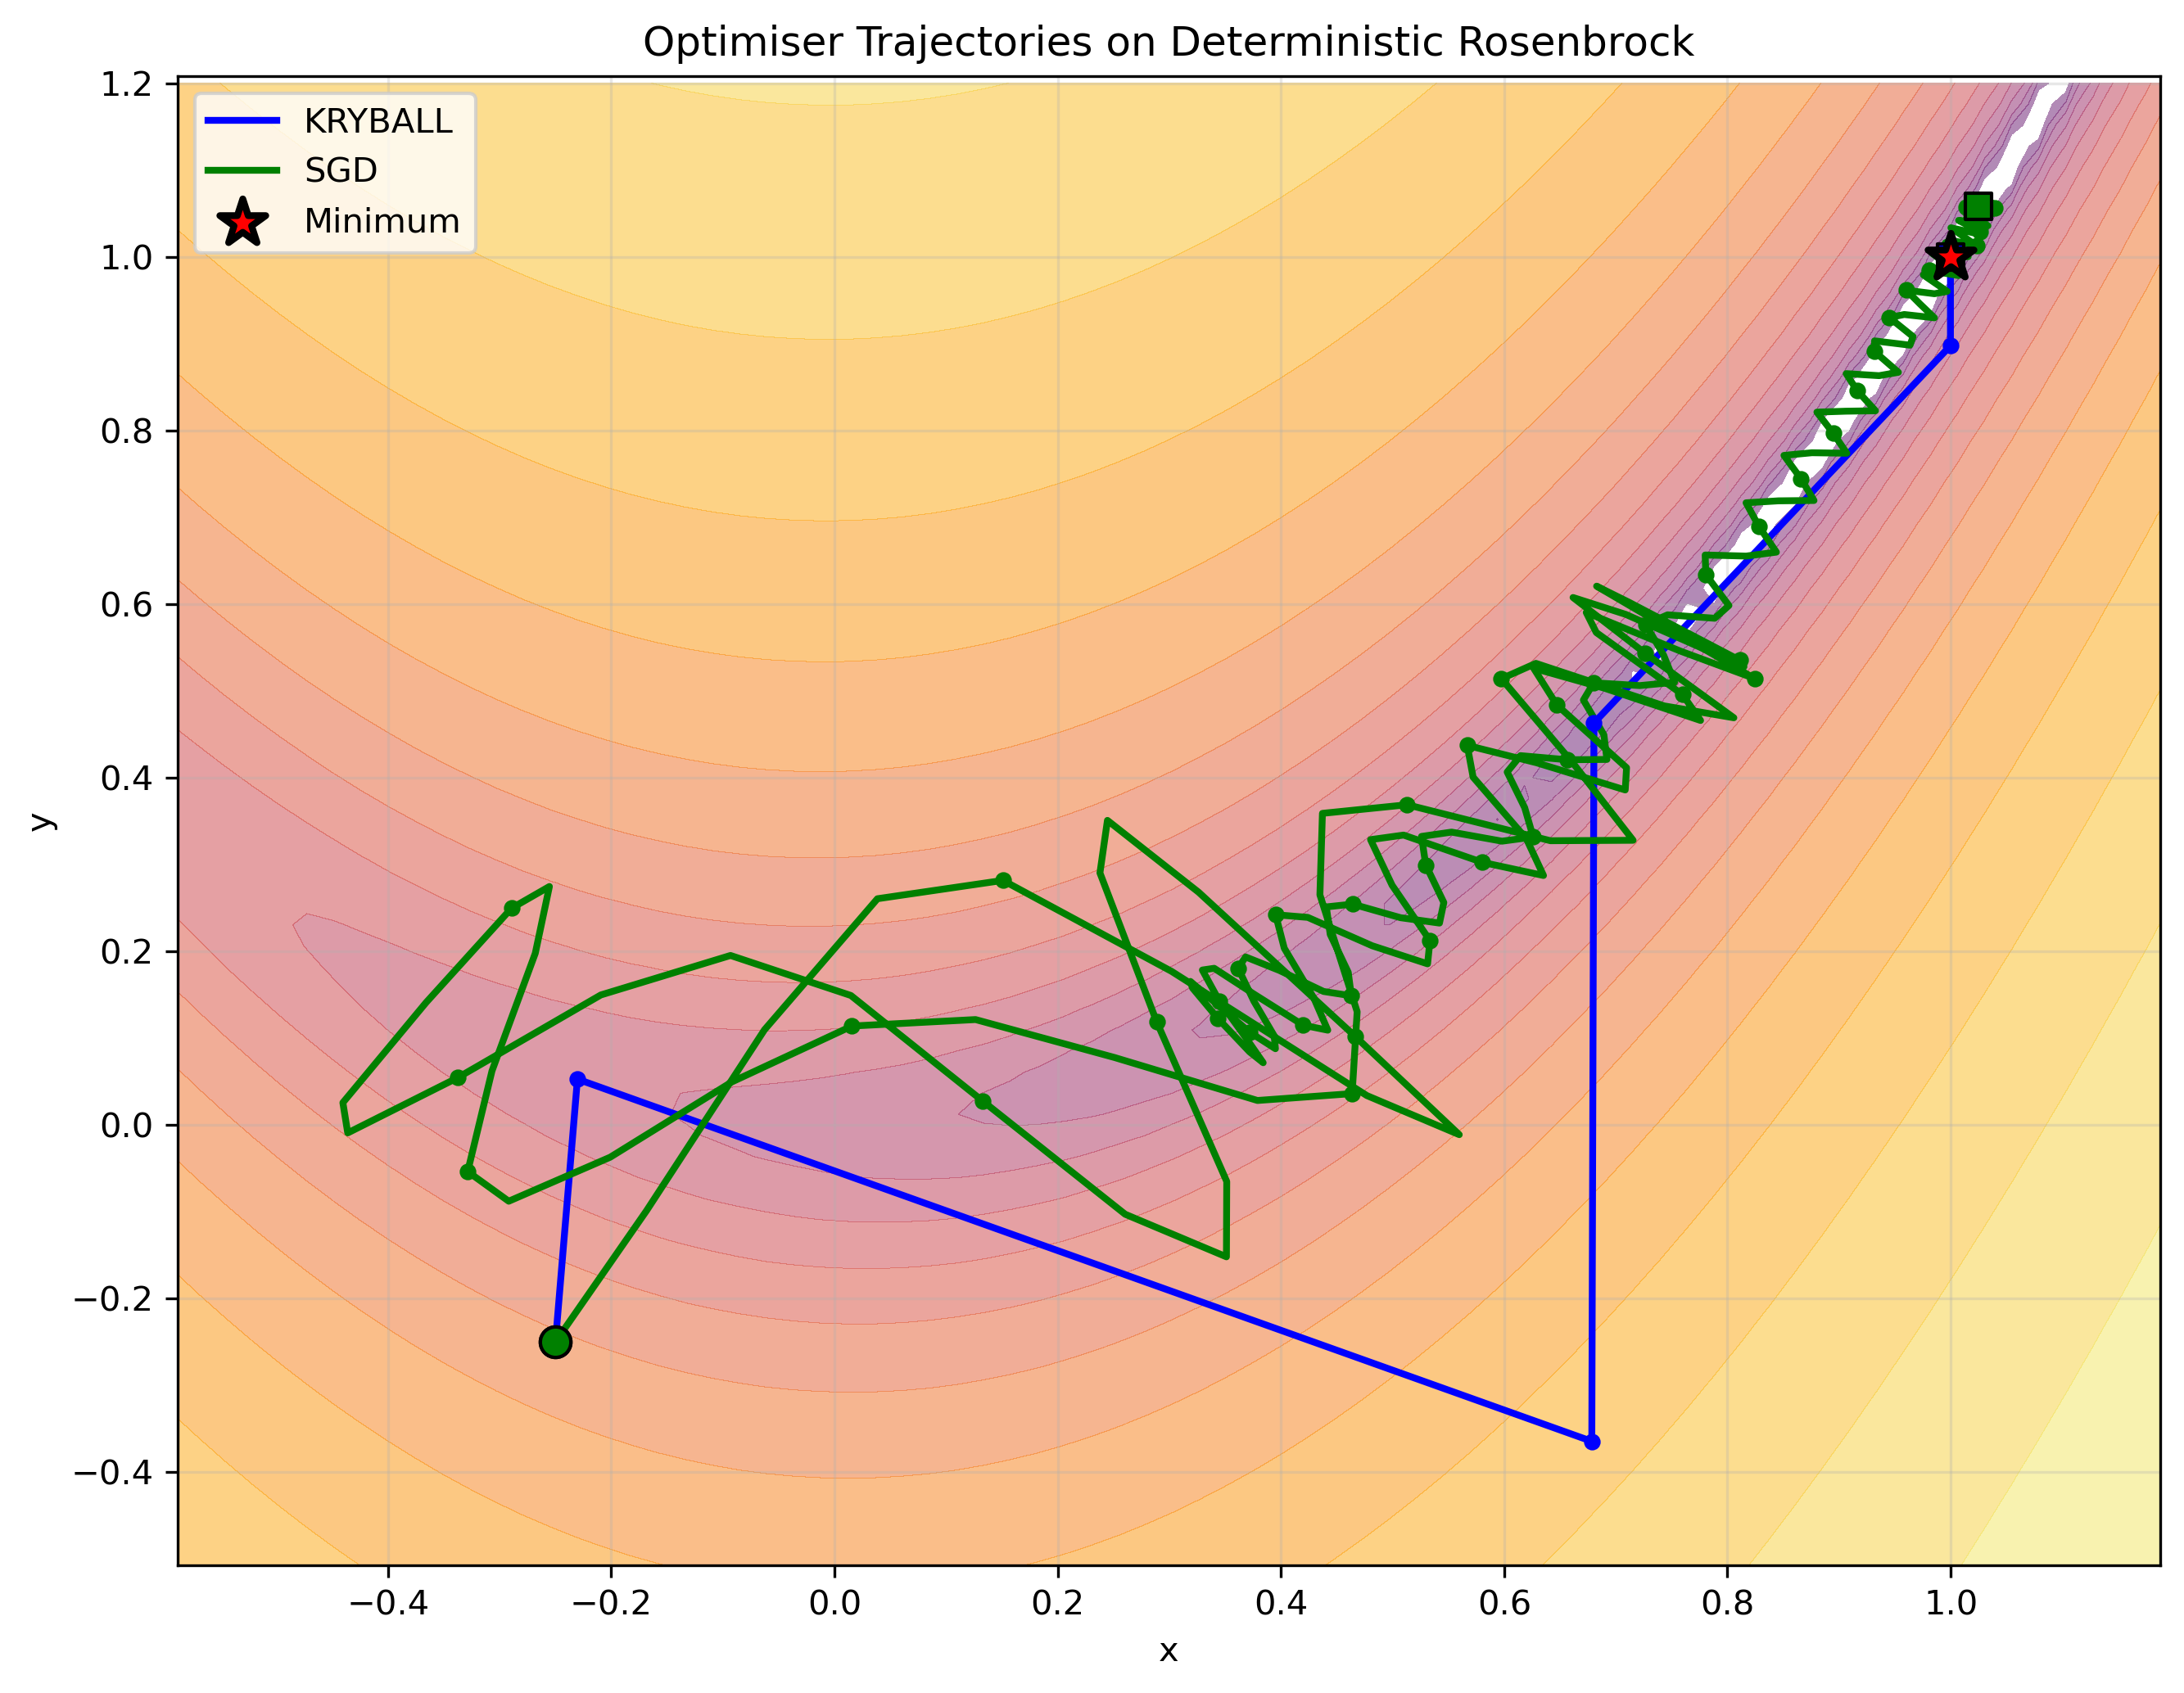
\includegraphics[width=\linewidth]{figures/5evals/deterministic.png}
        \caption{The optimiser trajectories on the deterministic Rosenbrock function with $\lambda_1 = 2$ and $\lambda_2 = 1$.}
        \label{fig:deterministic}
    \end{subfigure}
    \hfill
    \begin{subfigure}[b]{0.49\linewidth}
        \centering
        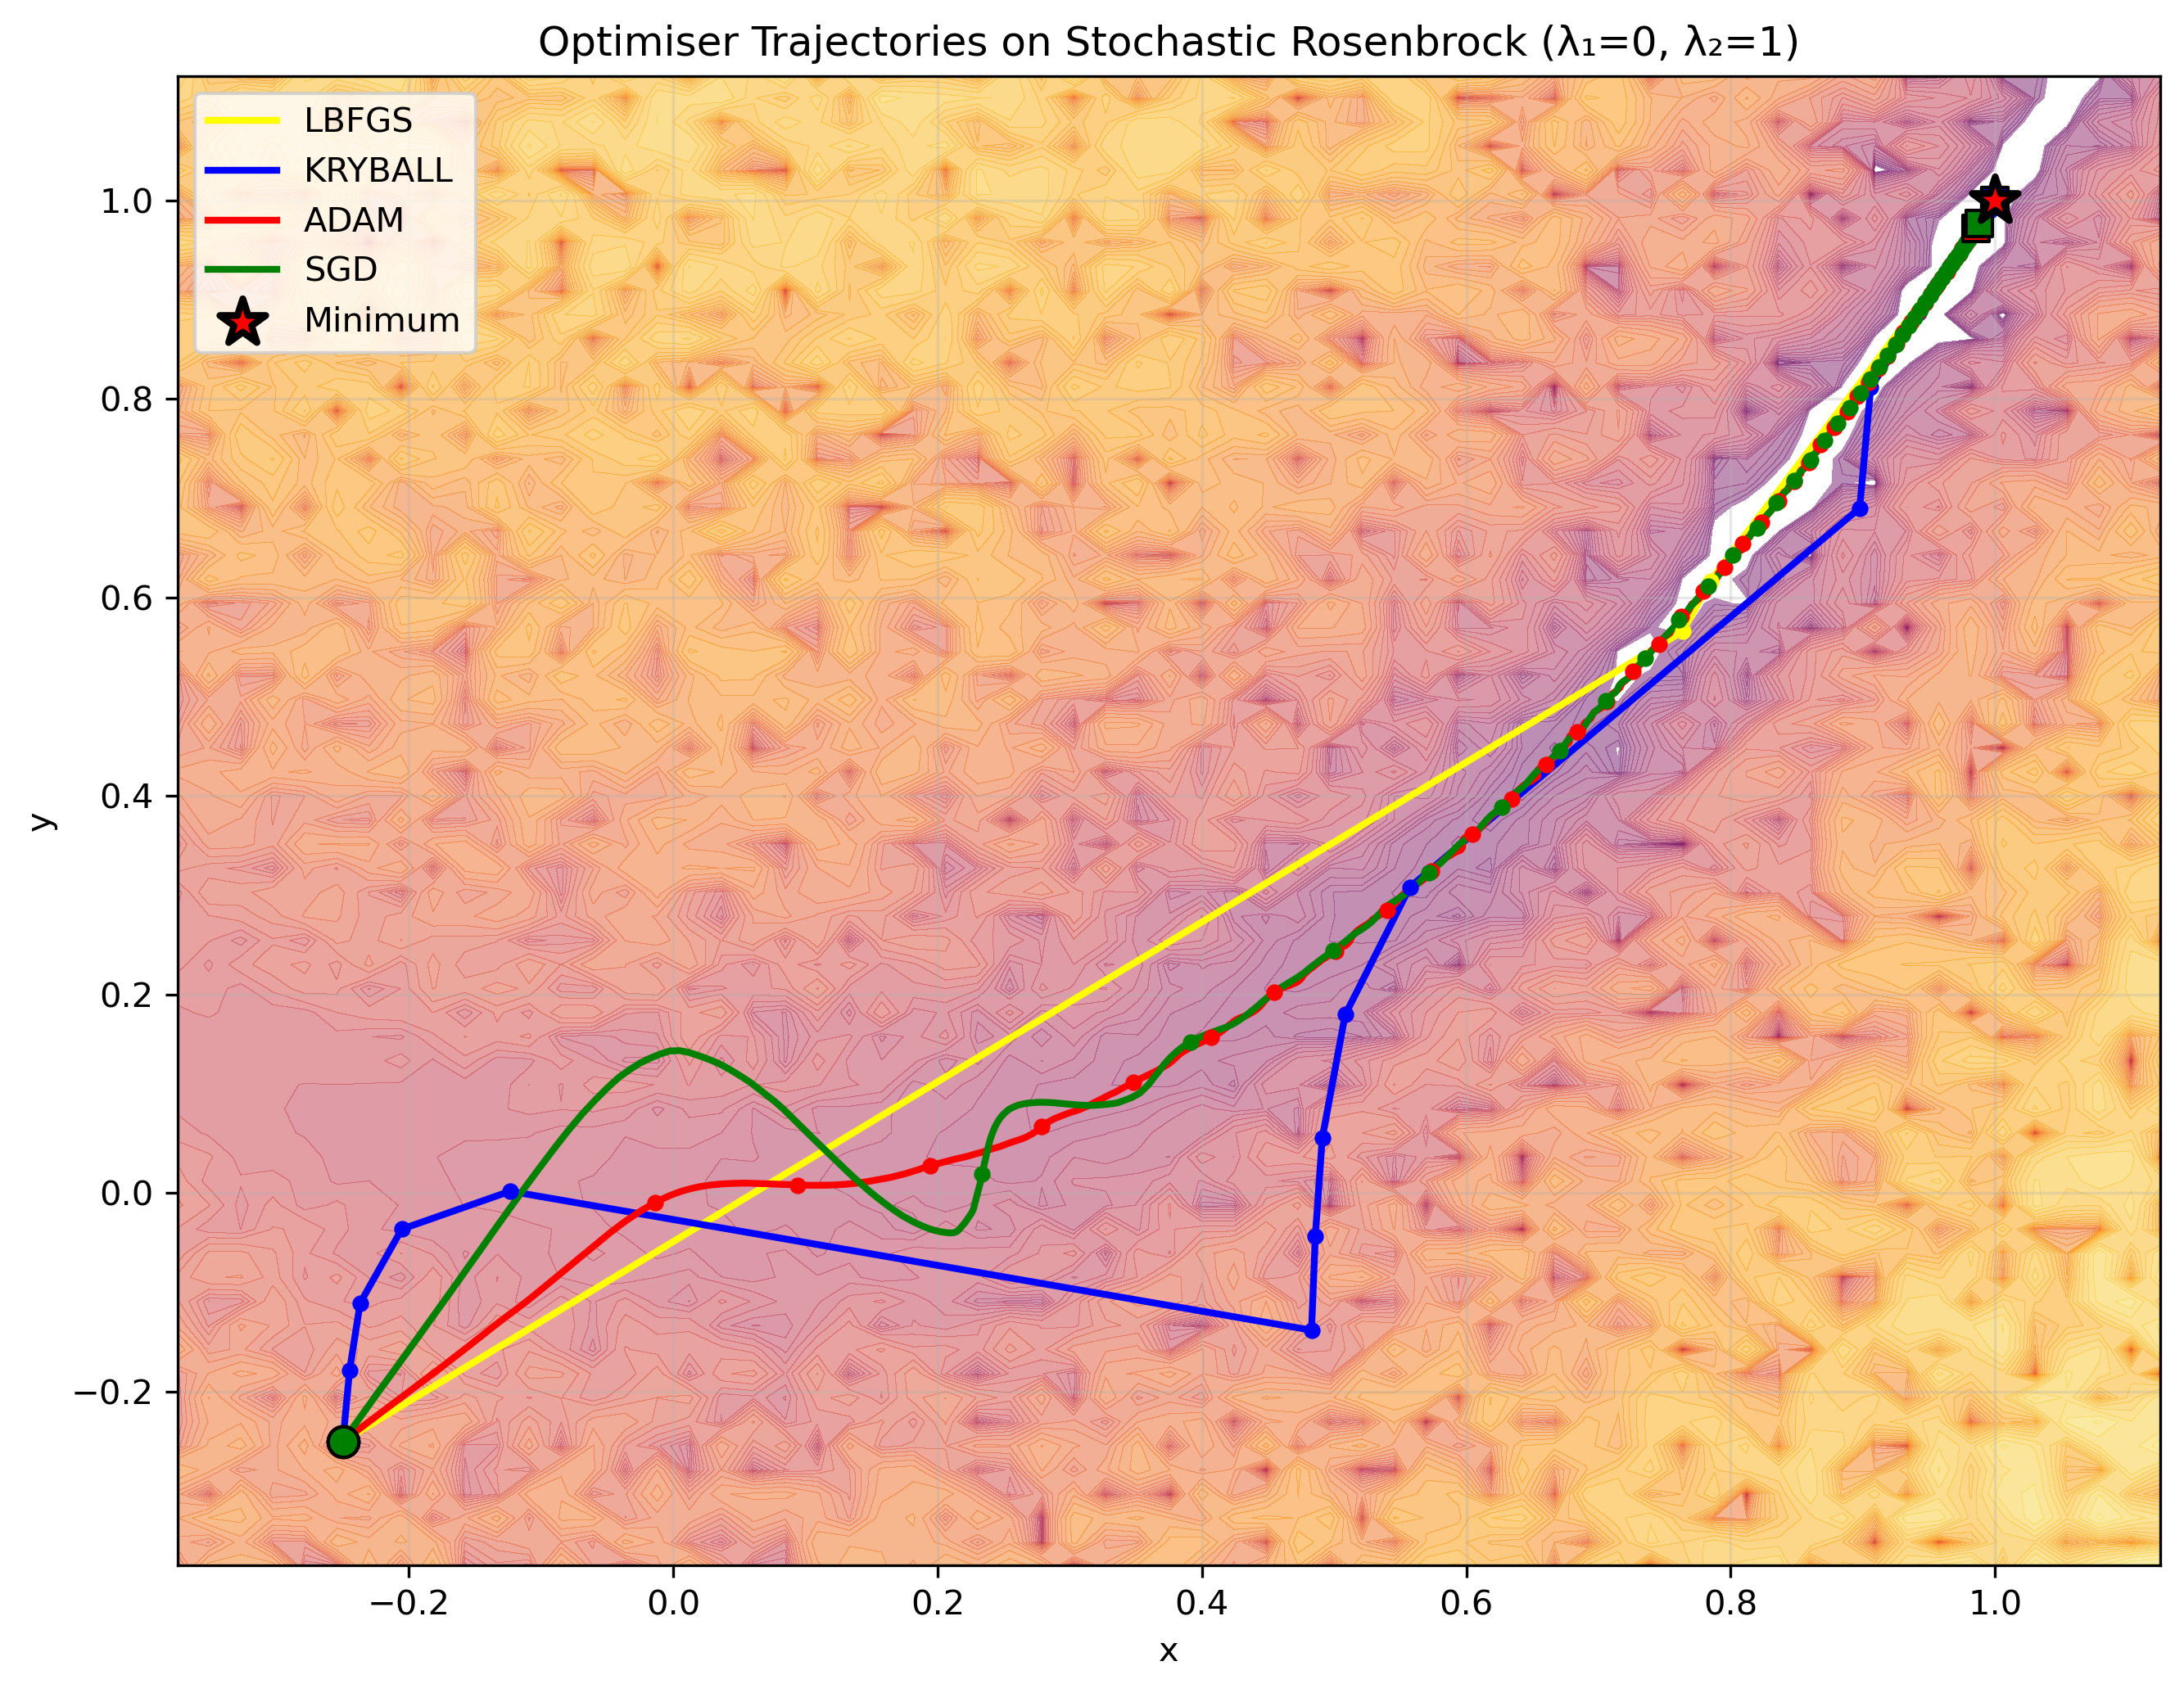
\includegraphics[width=\linewidth]{figures/5evals/stochastic_0_1.png}
        \caption{The optimiser trajectories on the stochastic Rosenbrock function with $\lambda_1 = 0$ and $\lambda_2 = 1$.}
        \label{fig:stochastic_1}
    \end{subfigure}
    
    \vspace{1em}

    \begin{subfigure}[b]{0.49\linewidth}
        \centering
        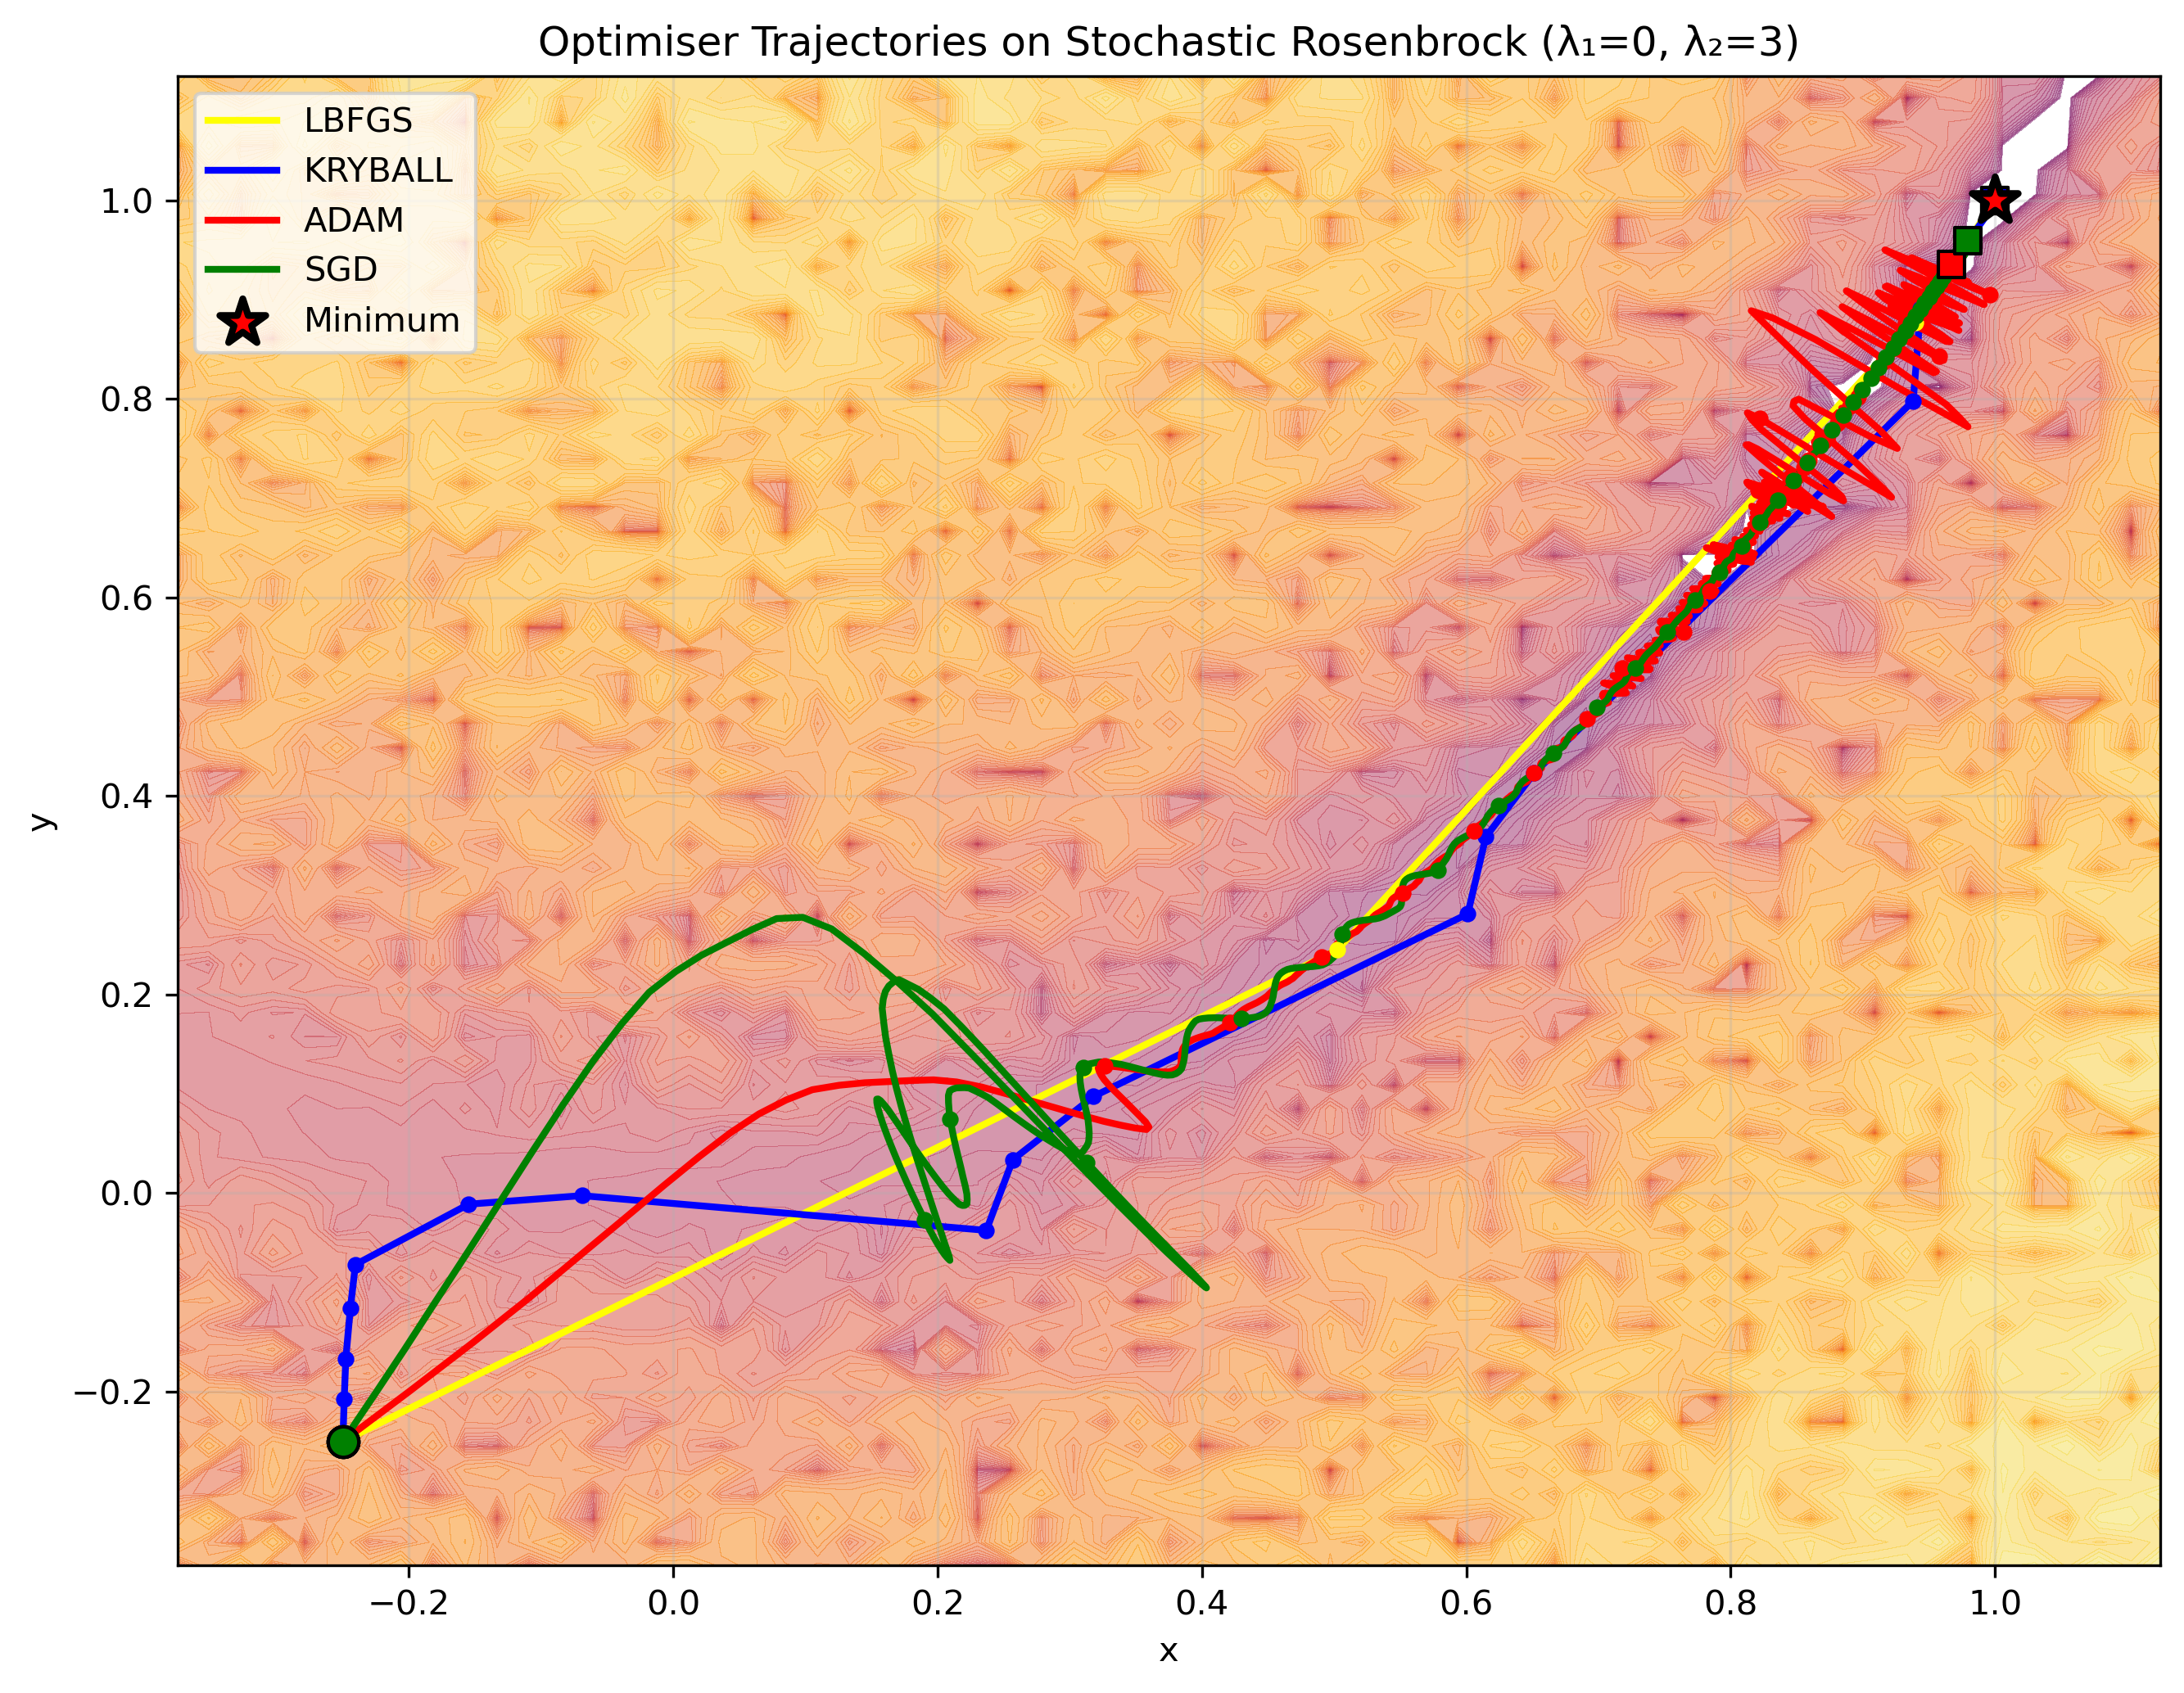
\includegraphics[width=\linewidth]{figures/5evals/stochastic_0_3.png}
        \caption{The optimiser trajectories on the stochastic Rosenbrock function with $\lambda_1 = 0$ and $\lambda_2 = 3$.}
        \label{fig:stochastic_2}
    \end{subfigure}
    \caption{The optimiser trajectories on the deterministic and stochastic Rosenbrock functions. KryBall and LBFGS are able to find the global minimum extremely quickly, and are not impacted by the ill-conditioning of the function. However, MSGD and Adam are impacted and converge much slower to the optimal solution.}
    \label{fig:rosenbrock_results}
\end{figure}

\begin{figure}[!t]
    \begin{subfigure}[b]{0.49\linewidth}
        \centering
        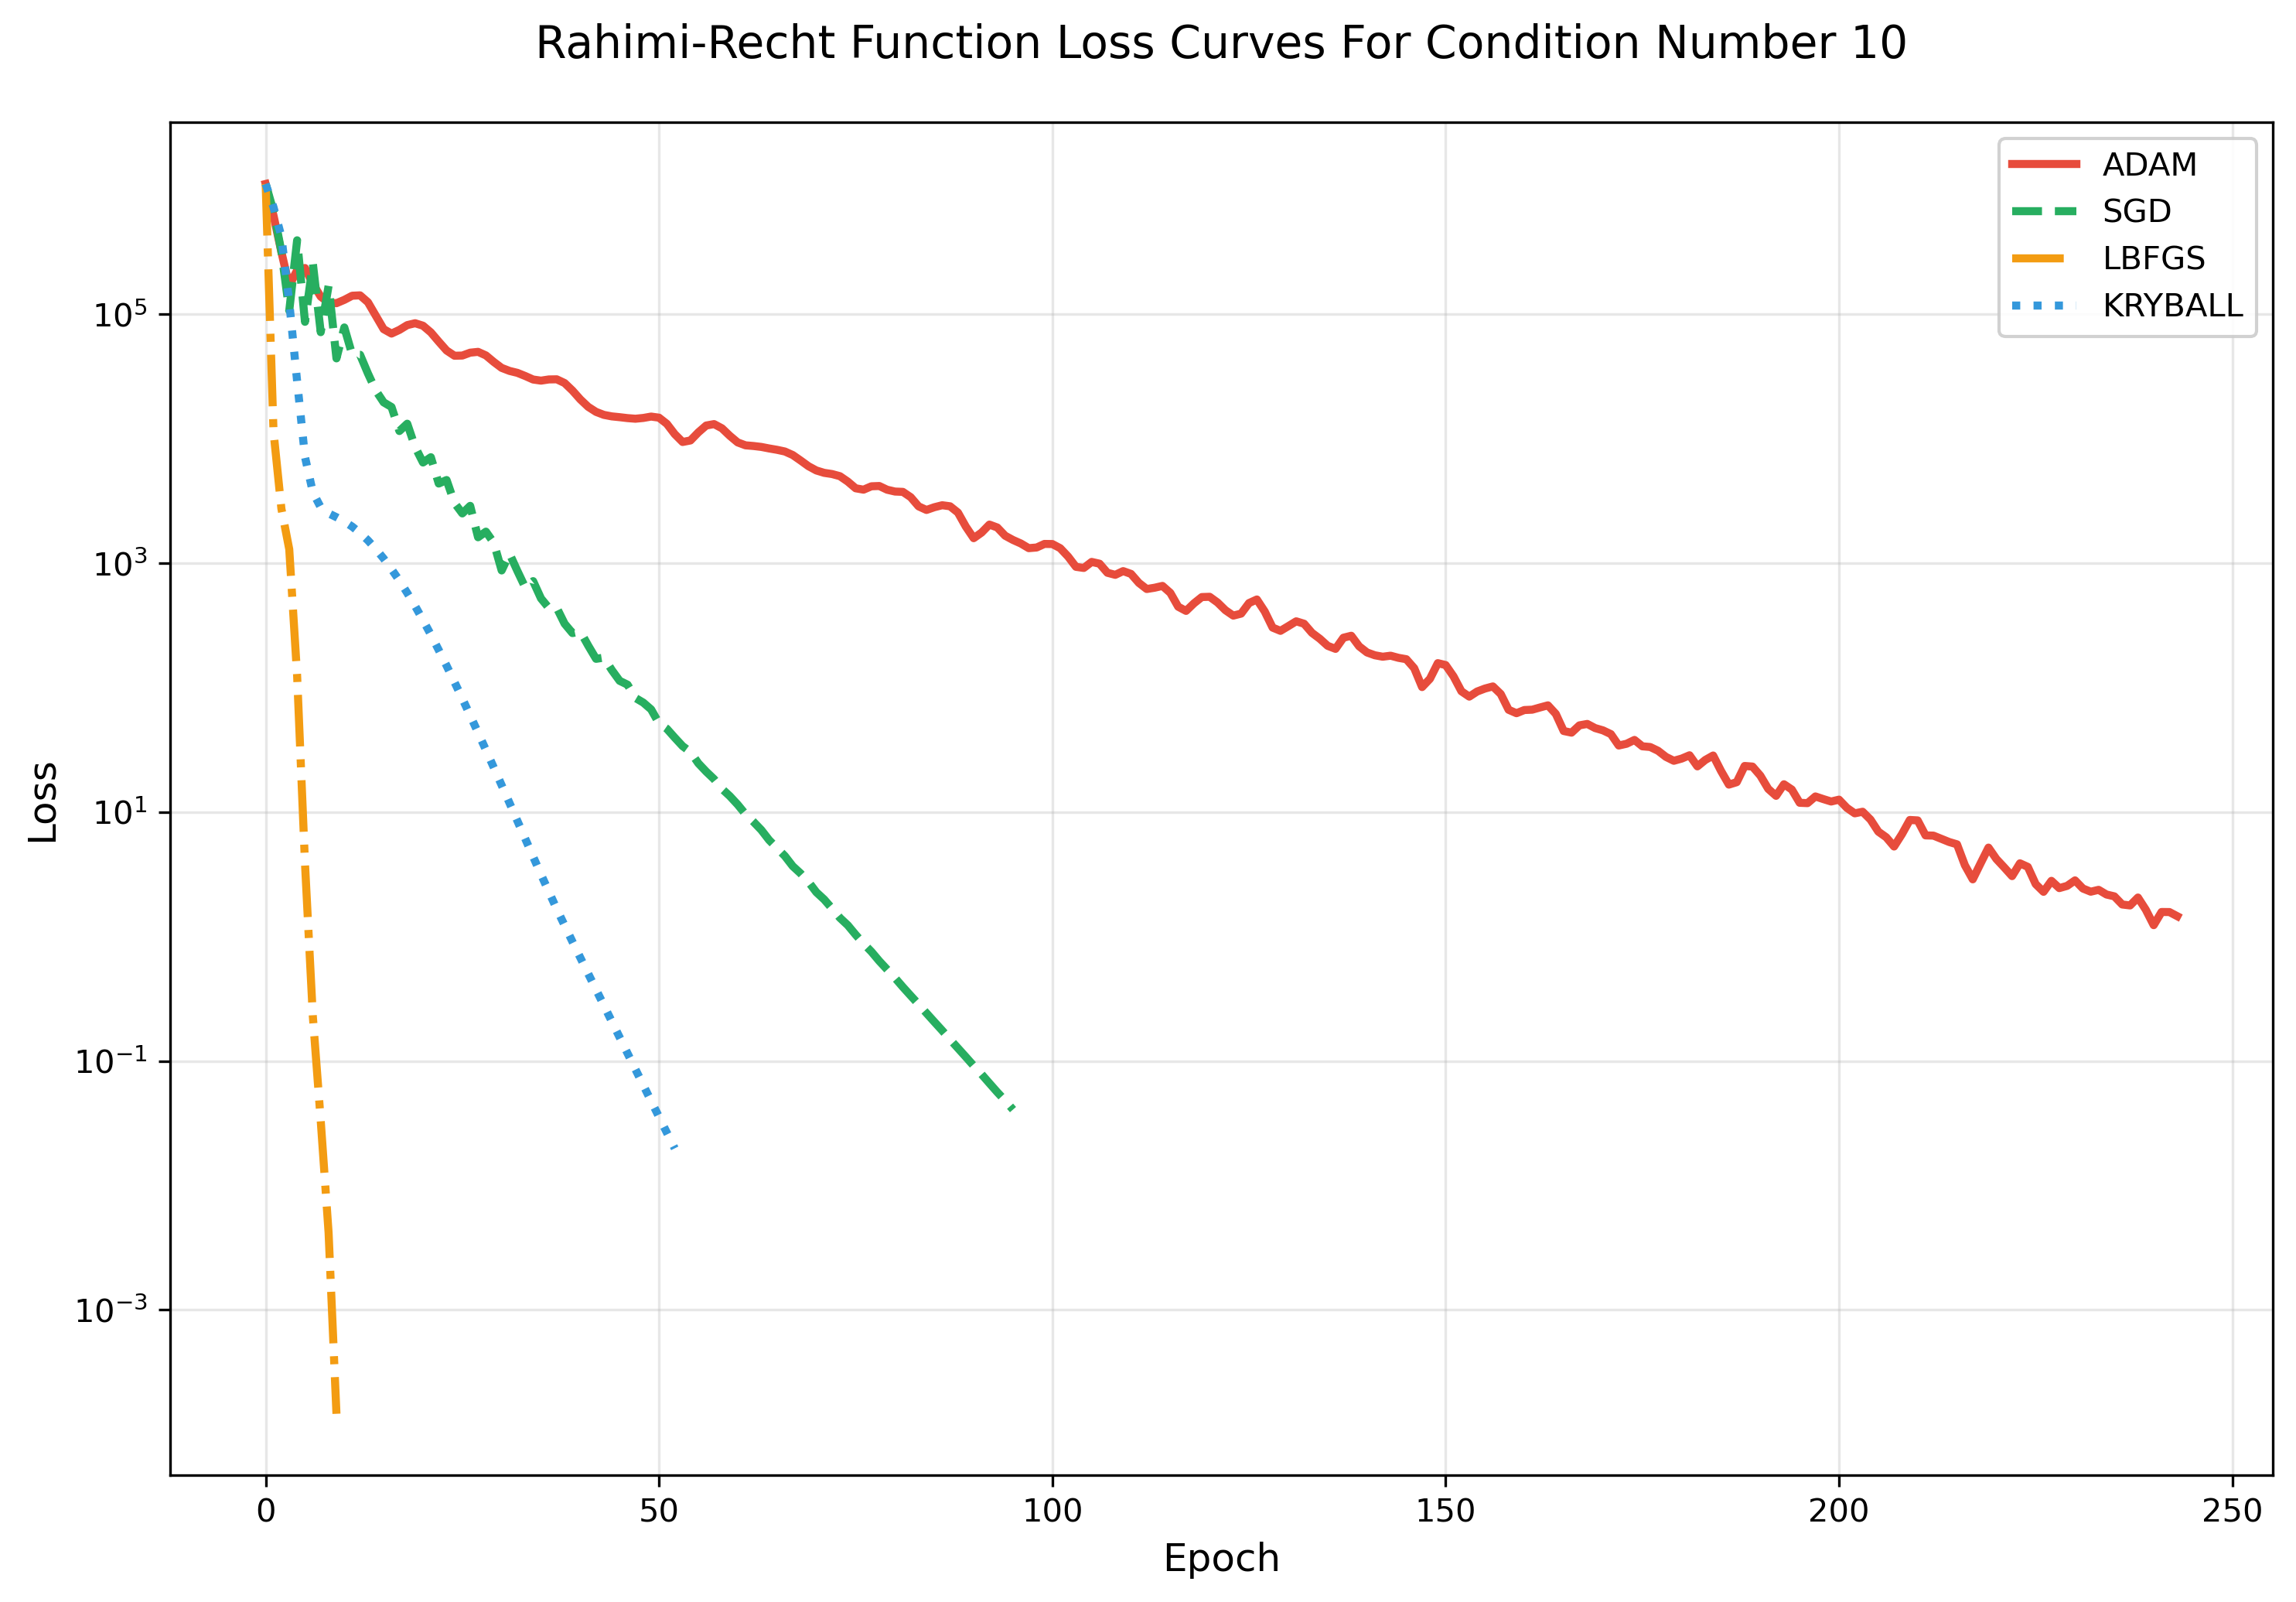
\includegraphics[width=\linewidth]{figures/5evals/rr_losses_k_10.png}
        \caption{Loss curves for the Rahimi-Recht function with condition number $\kappa = 10$.}
        \label{fig:rr_losses_k_10}
    \end{subfigure}
    \hfill
    \begin{subfigure}[b]{0.49\linewidth}
        \centering
        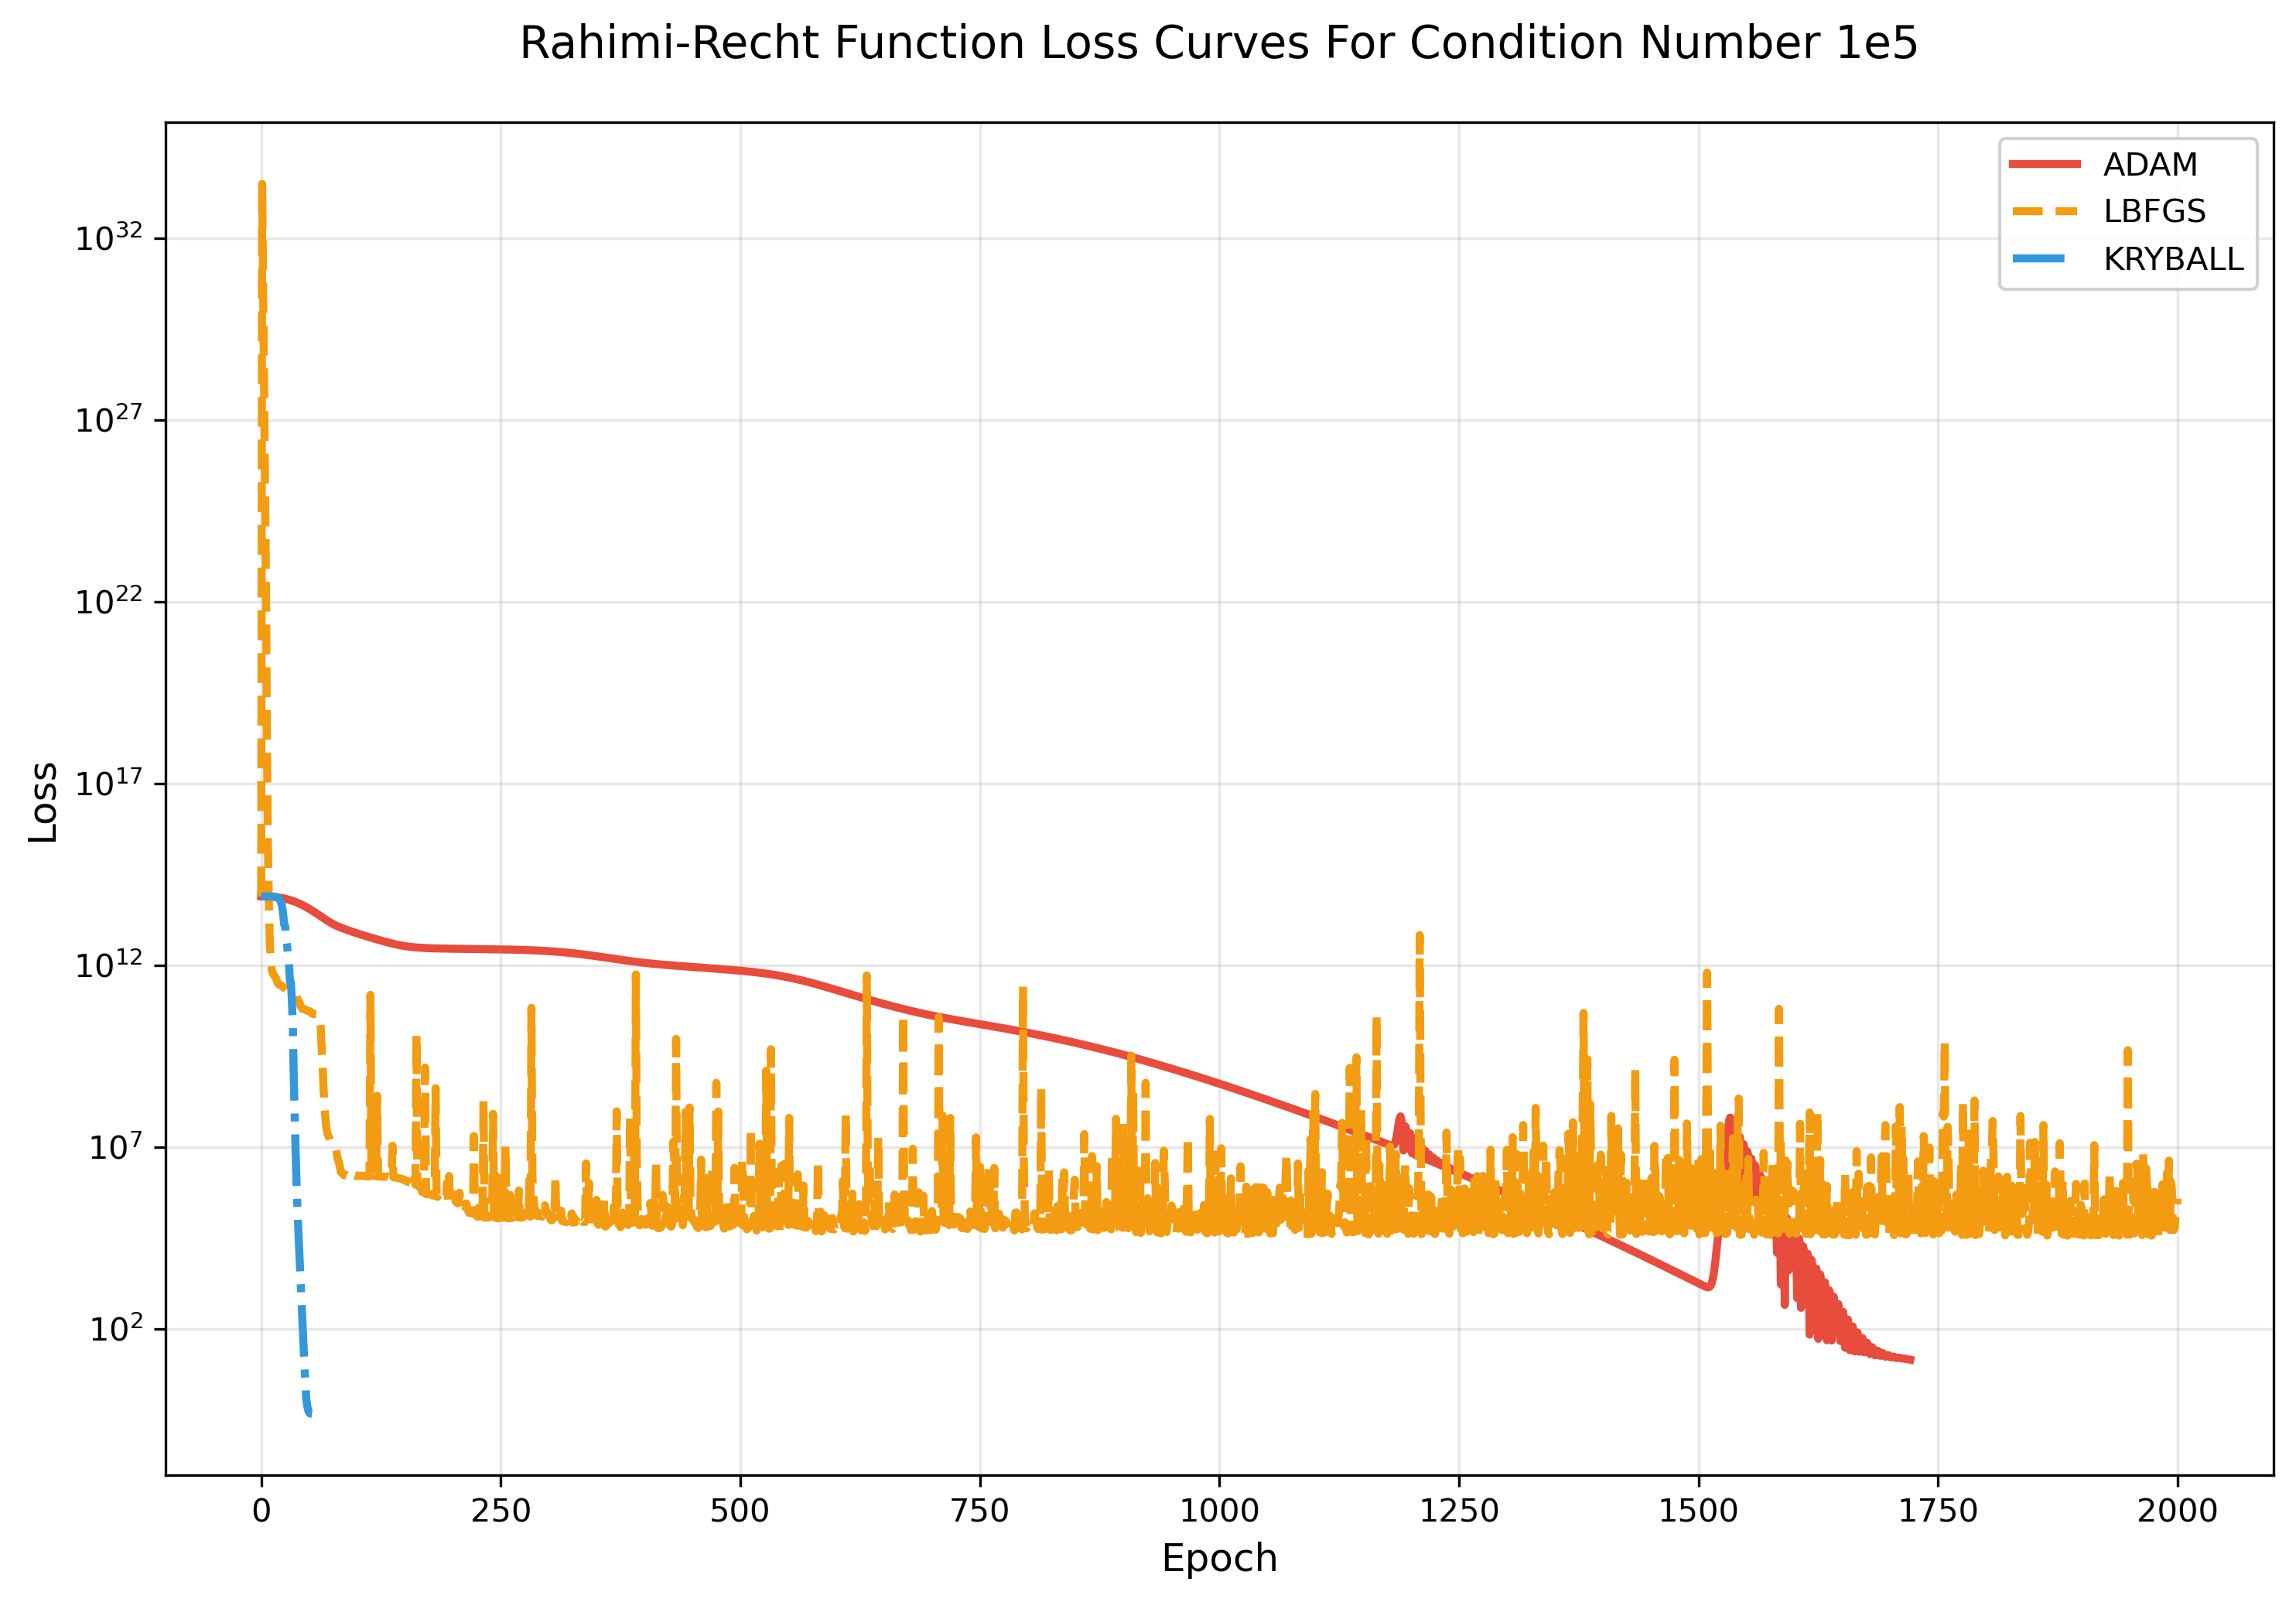
\includegraphics[width=\linewidth]{figures/5evals/rr_losses_k_1e5.png}
        \caption{Loss curves for the Rahimi-Recht function with condition number $\kappa = 1 \times 10^5$.}
        \label{fig:rr_losses_k_1e5}
    \end{subfigure}
    \caption{Loss curves for two instances of the Rahimi-Recht function. In \cref{fig:rr_losses_k_1e5}, we have slight degree of ill-conditioning with $\kappa = 10$, and in \cref{fig:rr_losses_k_10}, we have a very high degree of ill-conditioning with $\kappa = 1 \times 10^5$. We note that in \cref{fig:rr_losses_k_1e5}, MSGD is not here as it diverged in every run very quickly.}
    \label{fig:rr_results}
\end{figure}

\subsection{Task 2: XOR Classification}
\label{ssec:results_xor_classification}

We now move onto our second task, XOR classification. Here, we evaluate the performance of our optimisers based on how quickly the converge to zero loss. We note that here, LBFGS is limited to one evaluation per epoch to make it fair for all optimisers. This is because for many deep learning tasks, we no longer have a best case pratical scenario or upper bound and need to ensure a fair comparison.

\begin{figure}[!t]
    \centering
    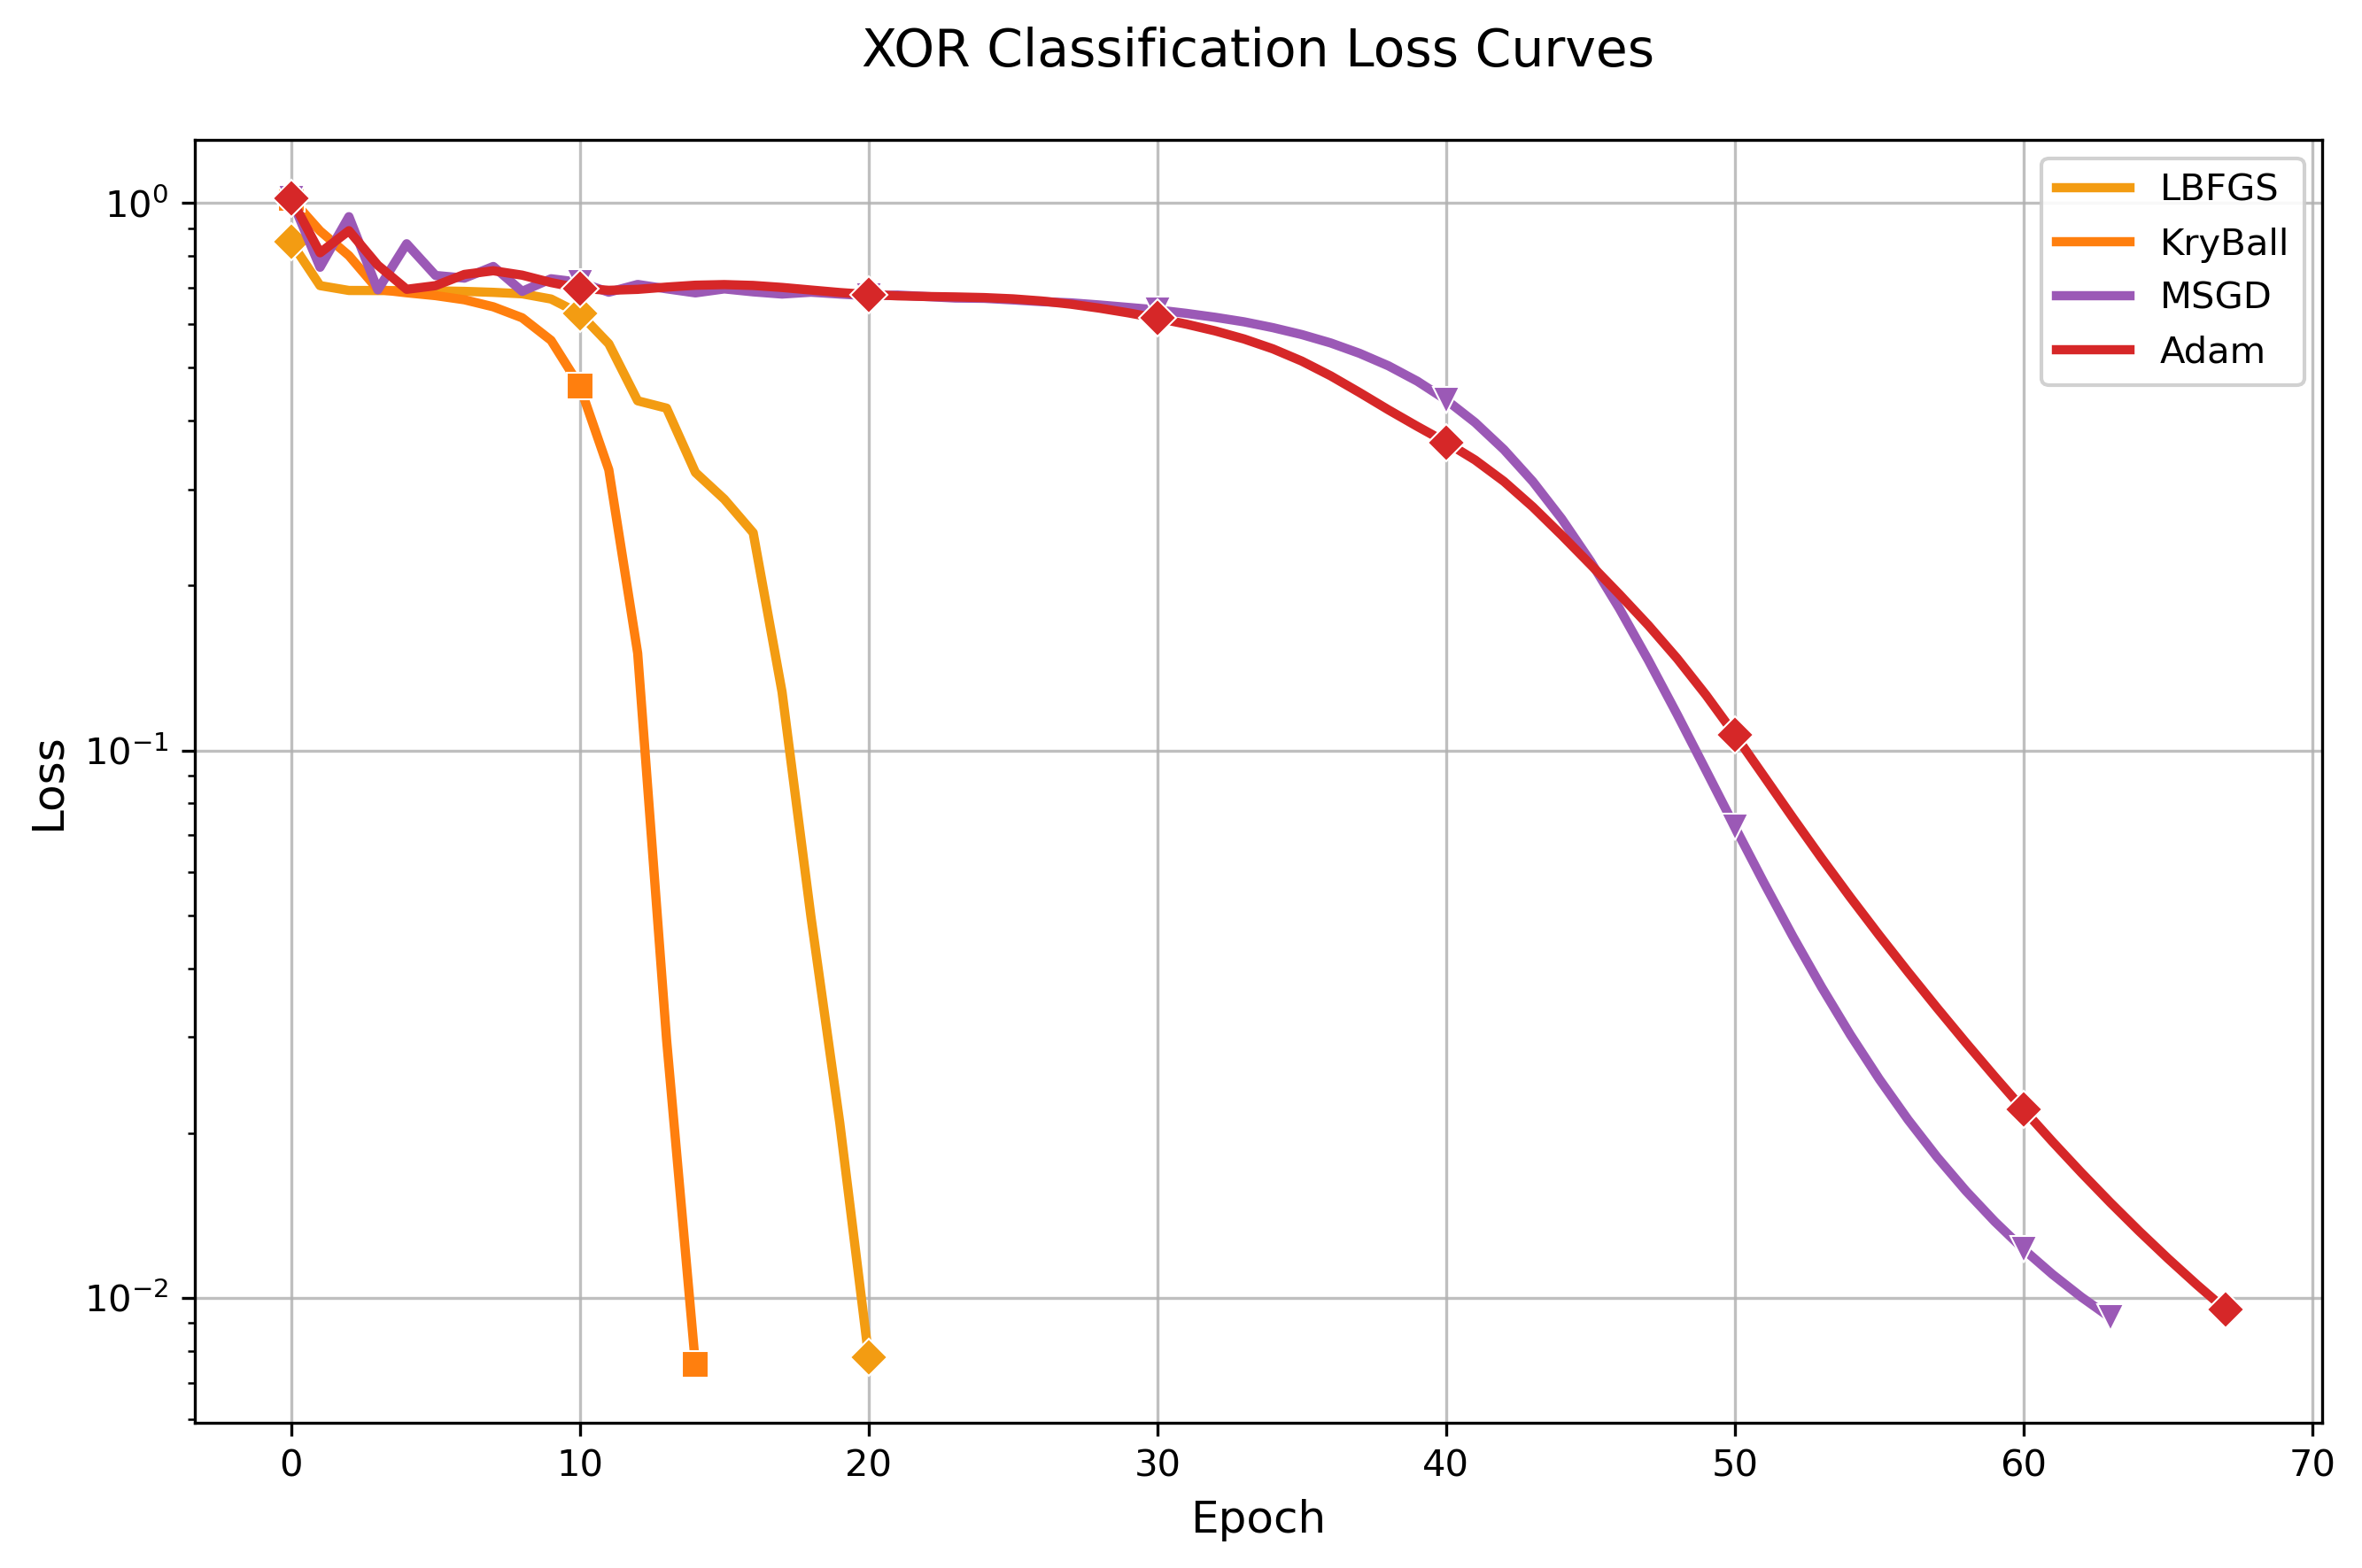
\includegraphics[width=0.6\linewidth]{figures/5evals/xor_losses.png}
    \caption{The loss curves for the XOR classification task. KryBall converges in 15 epochs, MSGD converges in 63 epochs and Adam converges to 67 epochs. LBFGS restricted to one evaluation per iteration converges in 20 epochs.}
    \label{fig:xor_results}
\end{figure}

\cref{fig:xor_results} shows the loss curves. We see that KryBall and LBFGS converge the quickest, in less than 25 epochs. MSGD and Adam are also able to converge, but take longer. This shows that KryBall is able to generalise very quickly, and that the second-order approximation is helpful in identifying the optimal solution. As such, this shows in the simplest setting that our approximation is useful in tasks where there are non-linearities involved. As we now transition into harder tasks that are highly parameterised and likely non-linear, we hypothesise that our quadratic model will be able to generalise and add more insight into the optimisation landscape.

We note that while this task is simple and may seem trivial, it is a good baseline and a bridge to more complex tasks in the next section. We now move onto these tasks in the next section.

\subsection{Task 3: Image Classification}
\label{ssec:results_image_classification}

We now move into the primary focus of our results, evaluating our optimiser on standard deep-learning tasks that are the benchmark for optimisers. We evaluate our optimisers on three image classification tasks: MNIST-1D, CIFAR-10 CNN, and CIFAR-10 ResNet-18, which we described in \cref{ssec:task_3_image_classification}. We note that from here onwards, we do not use LBFGS since it becomes too expensive and compute heavy to evaluate. Thus, our optimiser suite is now Adam, MSGD and KryBall. We present a summary of our results in \Cref{tab:classification_results}. Our loss curves and accuracies are provided in \cref{fig:image_classification_results}. 

% Please add the following required packages to your document preamble:
% \usepackage{multirow}
% \usepackage[table,xcdraw]{xcolor}
% Beamer presentation requires \usepackage{colortbl} instead of \usepackage[table,xcdraw]{xcolor}
\begin{table}[!t]
    \centering
    \caption{Classification results for MNIST1D MLP, CIFAR10 CNN, and CIFAR10 ResNet-18 given Adam, MSGD and KryBall optimisers.}
    \label{tab:classification_results}
    \begin{tabular}{ccccc}
    \hline
                                                                                            & \textbf{Method} & \textbf{\begin{tabular}[c]{@{}c@{}}Final \\ Training \\ Loss $\downarrow$\end{tabular}} & \textbf{\begin{tabular}[c]{@{}c@{}}Peak \\ Test\\ Accuracy $\uparrow$\end{tabular}} & \textbf{\begin{tabular}[c]{@{}c@{}}Final \\ Test\\ Accuracy $\uparrow$\end{tabular}} \\ \hline
                                                                                            & Adam            & \cellcolor[HTML]{FFFFFF}0.144                                              & \cellcolor[HTML]{FFFFFF}0.668                                            & \cellcolor[HTML]{FFFFFF}0.668                                             \\
                                                                                            & MSGD            & \cellcolor[HTML]{FFFFFF}0.326                                              & \cellcolor[HTML]{FFFFFF}0.669                                            & \cellcolor[HTML]{FFFFFF}0.644                                             \\
    \multirow{-3}{*}{\textbf{\begin{tabular}[c]{@{}c@{}}MNIST1D\\ MLP\end{tabular}}}        & KryBall         & \cellcolor[HTML]{34FF34}\textbf{0.001}                                     & \cellcolor[HTML]{34FF34}\textbf{0.685}                                   & \cellcolor[HTML]{34FF34}\textbf{0.685}                                    \\ \hline
                                                                                            & Adam            & \cellcolor[HTML]{34FF34}\textbf{0.099}                                     & 0.782                                                                    & \cellcolor[HTML]{34FF34}\textbf{0.777}                                    \\
                                                                                            & MSGD            & 0.111                                                                      & 0.777                                                                    & 0.771                                                                     \\
    \multirow{-3}{*}{\textbf{\begin{tabular}[c]{@{}c@{}}CIFAR10 \\ CNN\end{tabular}}}       & KryBall         & 0.135                                                                      & \cellcolor[HTML]{34FF34}\textbf{0.783}                                   & 0.762                                                                     \\ \hline
                                                                                            & Adam            & \cellcolor[HTML]{34FF34}\textbf{7.5e-5}                                    & \cellcolor[HTML]{34FF34}\textbf{0.843}                                   & \cellcolor[HTML]{34FF34}\textbf{0.842}                                    \\
                                                                                            & MSGD            & 1e-4                                                                       & 0.832                                                                    & 0.829                                                                     \\
    \multirow{-3}{*}{\textbf{\begin{tabular}[c]{@{}c@{}}CIFAR10 \\ ResNet-18\end{tabular}}} & KryBall         & 0.002                                                                      & 0.832                                                                    & 0.822                                                                     \\ \hline
    \end{tabular}
    \end{table}

\begin{figure}[!t]
    \centering
    % First column
    \begin{subfigure}[b]{0.48\linewidth}  % Wider subfigures (0.48 instead of 0.32)
        \centering
        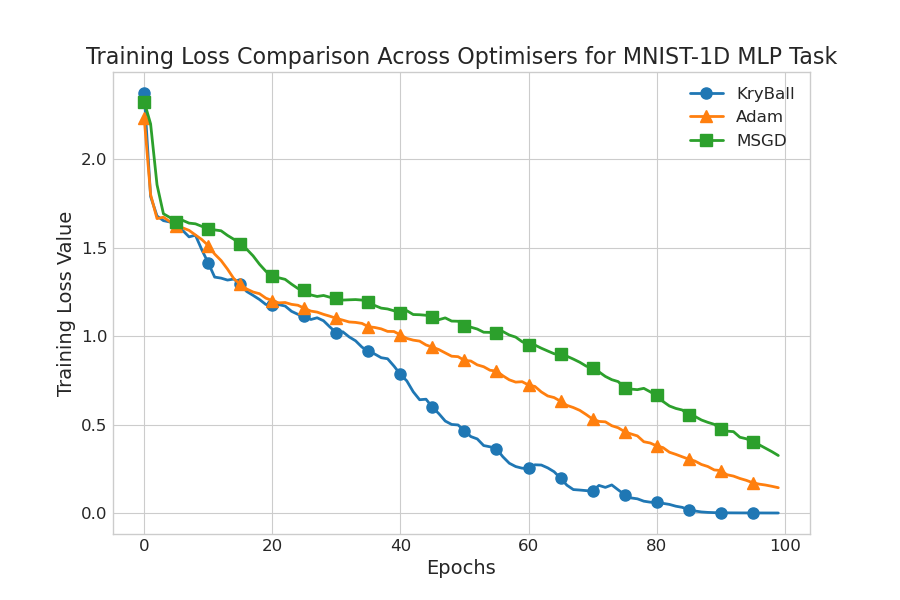
\includegraphics[width=\linewidth]{figures/5evals/mnist1d_mlp_loss.png}
        \caption{Training Loss on MNIST-1D MLP}
        \label{fig:mnist1d_mlp_loss}
    \end{subfigure}
    \begin{subfigure}[b]{0.48\linewidth}
        \centering
        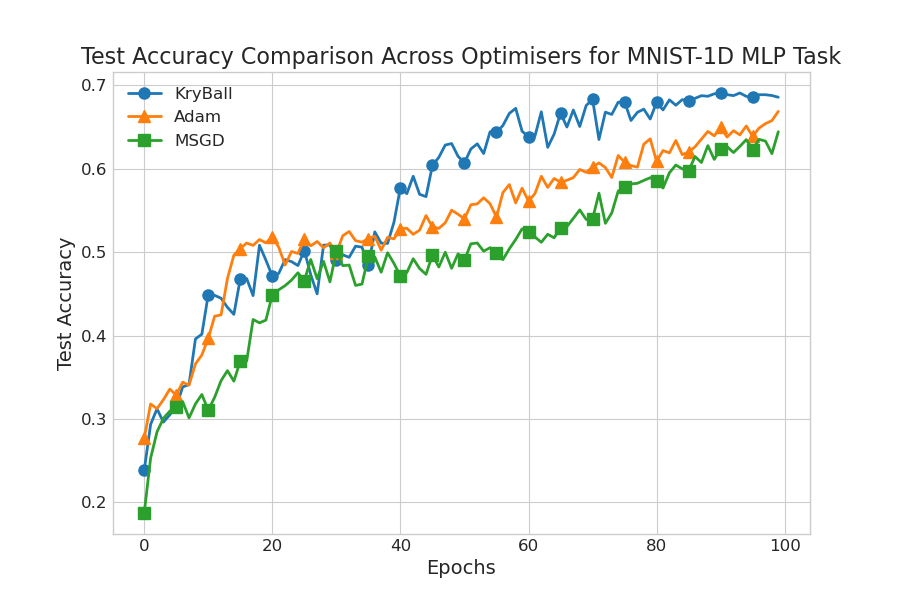
\includegraphics[width=\linewidth]{figures/5evals/mnist1d_mlp_acc.png}
        \caption{Training Accuracy on MNIST-1D MLP}
        \label{fig:mnist1d_mlp_acc}
    \end{subfigure}
    
    \vspace{1em}  % Add vertical space between rows
    
    % Second row
    \begin{subfigure}[b]{0.45\linewidth}
        \centering
        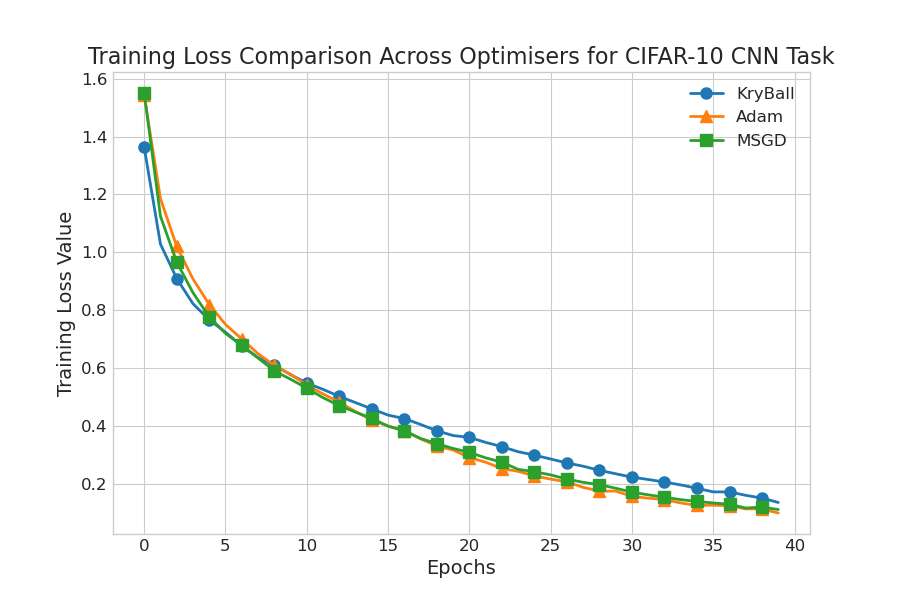
\includegraphics[width=\linewidth]{figures/5evals/cifar10_cnn_loss.png}
        \caption{Training Loss on CIFAR-10 CNN}
        \label{fig:cifar10_cnn_loss}
    \end{subfigure}
    \hfill
    \begin{subfigure}[b]{0.48\linewidth}
        \centering
        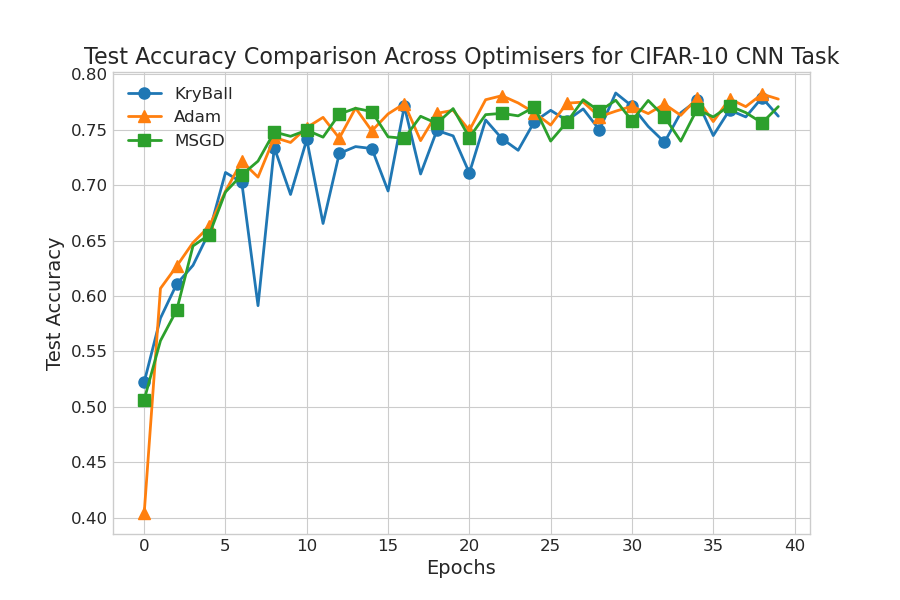
\includegraphics[width=\linewidth]{figures/5evals/cifar10_cnn_acc.png}
        \caption{Training Accuracy on CIFAR-10 CNN}
        \label{fig:cifar10_cnn_acc}
    \end{subfigure}
    
    \vspace{1em}  % Add vertical space between rows
    
    % Third row
    \begin{subfigure}[b]{0.48\linewidth}
        \centering
        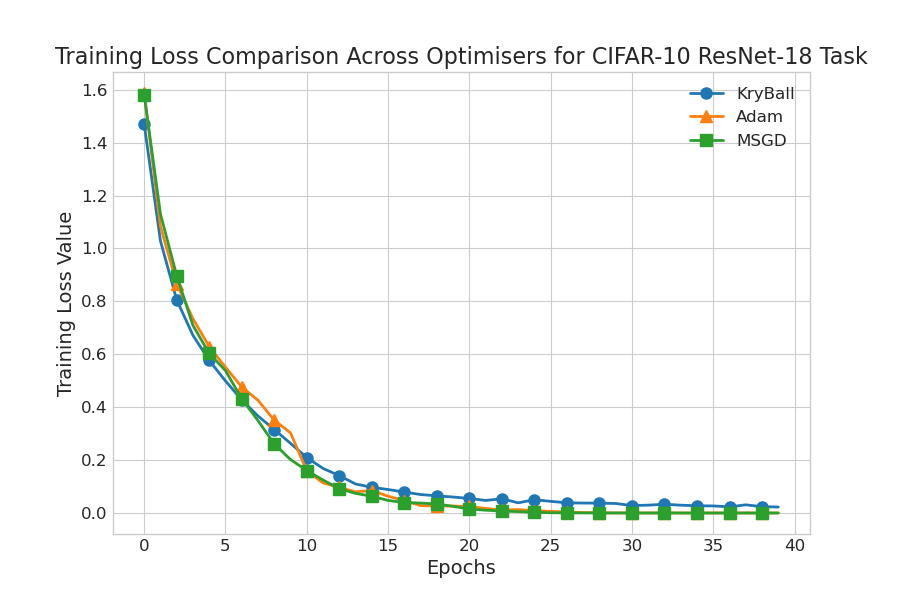
\includegraphics[width=\linewidth]{figures/5evals/cifar10_resnet_loss.png}  % Replace with actual duplicate figure
        \caption{Training Loss on CIFAR-10 ResNet-18}
        \label{fig:cifar10_resnet_loss}
    \end{subfigure}
    \hfill
    \begin{subfigure}[b]{0.48\linewidth}
        \centering
        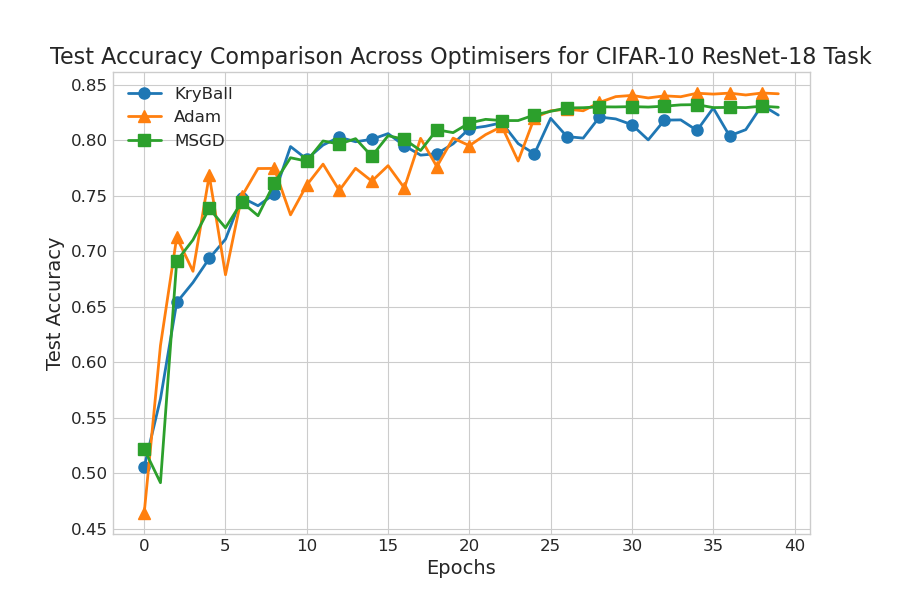
\includegraphics[width=\linewidth]{figures/5evals/cifar10_resnet_acc.png}  % Replace with actual duplicate figure
        \caption{Training Accuracy on CIFAR-10 ResNet-18}
        \label{fig:cifar10_resnet_acc}
    \end{subfigure}
    
    \caption{Loss curves and test accuracy comparisons among our image classification tasks consisting of MNIST-1D MLP, CIFAR-10 CNN and CIFAR-10 ResNet-18. Each task is evaluated with KryBall, Adam and MSGD.}
    \label{fig:image_classification_results}
\end{figure}

\textbf{MNIST-1D MLP}: KryBall demonstrates a clear advantage for the MNIST-1D MLP task. It is able to achieve the highest peak accuracy and the lowest final training loss. \cref{fig:mnist1d_mlp_loss} and \cref{fig:mnist1d_mlp_acc} show that KryBall converges quickly and makes a large improvement over Adam and MSGD, especially in 40 to 80 epoch range. We note that while a peak accuracy of 0.685 may not sound high, this contends with the best result on this specific model for MNIST-1D \cite{greydanus_mnist1d}. As such, we outperform Adam and MSGD in all metrics.

\textbf{CIFAR-10 CNN}: Here, we see a more nuanced performance. Adam achieves the lowest final training loss, alongside the best final test accuracy. However, KryBall slightly outperforms Adam and records a higher peak test accuracy. The training loss curves in \cref{fig:cifar10_cnn_loss} show Adam and MSGD reaching a slightly lower loss plateau than KryBall. In terms of test accuracy curves in \cref{fig:cifar10_cnn_acc}, all three optimisers are competitive, with KryBall showing a strong peak but Adam and MSGD achieve slightly better peak test accuracy. A key observation here is that in \cref{fig:cifar10_cnn_acc}, KryBall originally has a lower training loss, but then is surpassed by Adam and MSGD as training continue. During epochs 10 to 25, KryBall is also quite variant before converging. This is unlike Adam and MSGD, who are consistent all the way. 

\textbf{CIFAR-10 ResNet-18}: We see a similar comparison here. Adam has the best final training loss, and best peak test and final test accuracy. However, KryBall is generally competitive with Adam and MSGD. It achieves the same best test accuracy as MSGD, and only a slightly lower final test accuracy. Furthermore, \cref{fig:cifar10_resnet_loss} shows the same trend as in \cref{fig:cifar10_cnn_loss}, where KryBall is initially competitive and achieves a lower training loss, but then is surpassed by Adam and MSGD as training continues. In \cref{fig:cifar10_resnet_acc}, we see that KryBall is more stable than Adam and MSGD in the earlier epochs, but less stable in the later epochs and thus its performance suffers. The late epoch instability is also seen in \cref{fig:cifar10_cnn_acc}. 

To recap, KryBall outperforms the state-of-the art Adam and MSGD on the MNIST-1D MLP task, but does not outperform them on the CIFAR-10 tasks. More interestingly, we see that KryBall achieves lower training loss initially in all tasks early on, but then is surpassed by Adam and MSGD as training continues for the CIFAR-10 tasks. Near the end of training, KryBall is less stable than Adam and MSGD and is more variant. We discuss this further in\cref{sec:discussion_and_further_analysis}.

\subsection{Sensitivity Analysis}
\label{ssec:sensitivity_analysis}

We now perform a sensitivity analysis of our method on the MNIST-1D MLP task. We choose this since it is our best performing task. Our sensitive analysis is on the Krylov subspace dimension $M$ and the krylov refresh rate $r_{\mathit{refresh}}$. This is done by varying $M$ and $r_{\mathit{refresh}}$ from their hyperparameter ranges and keeping all other hyperparameters constant. We present the results in \cref{fig:sensitivity_analysis}.

\begin{figure}[!t]
    \begin{subfigure}[b]{0.49\linewidth}
        \centering
        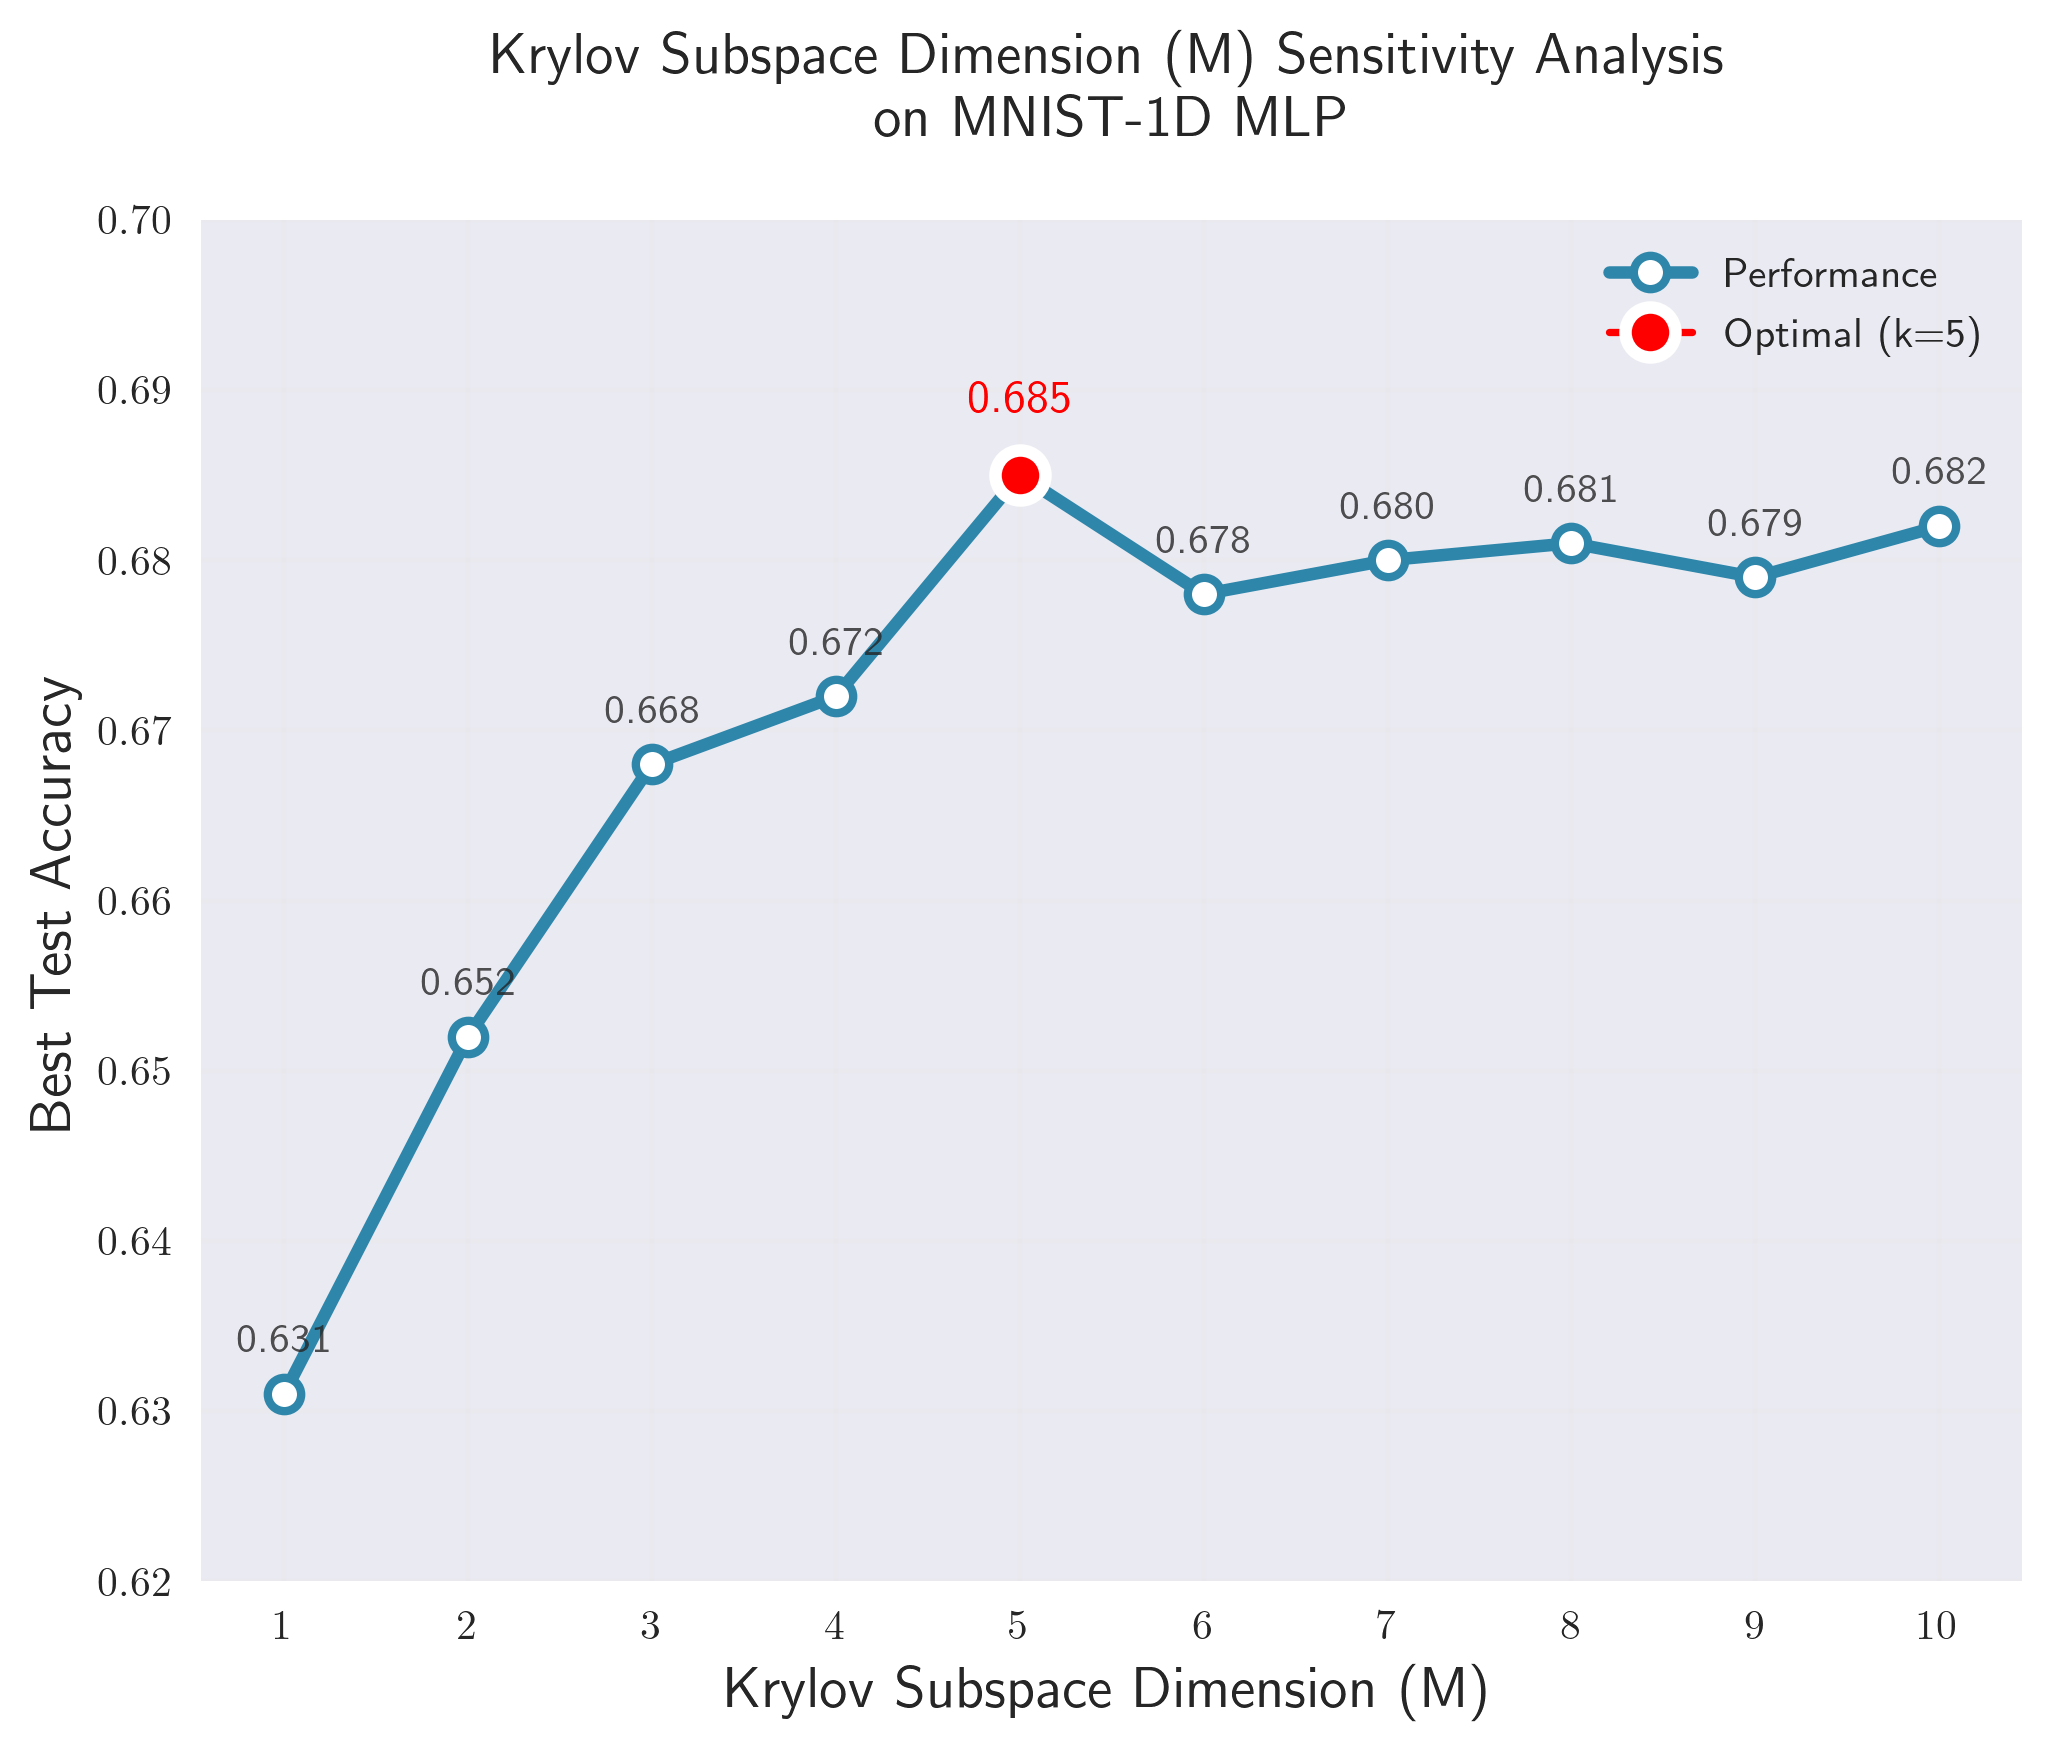
\includegraphics[width=\linewidth]{figures/5evals/sens_krylov_dim.png}
        \caption{The sensitivity analysis of the Krylov subspace dimension $M$ on MNIST-1D MLP.}
        \label{fig:sens_krylov_dim}
    \end{subfigure}
    \hfill
    \begin{subfigure}[b]{0.49\linewidth}
        \centering
        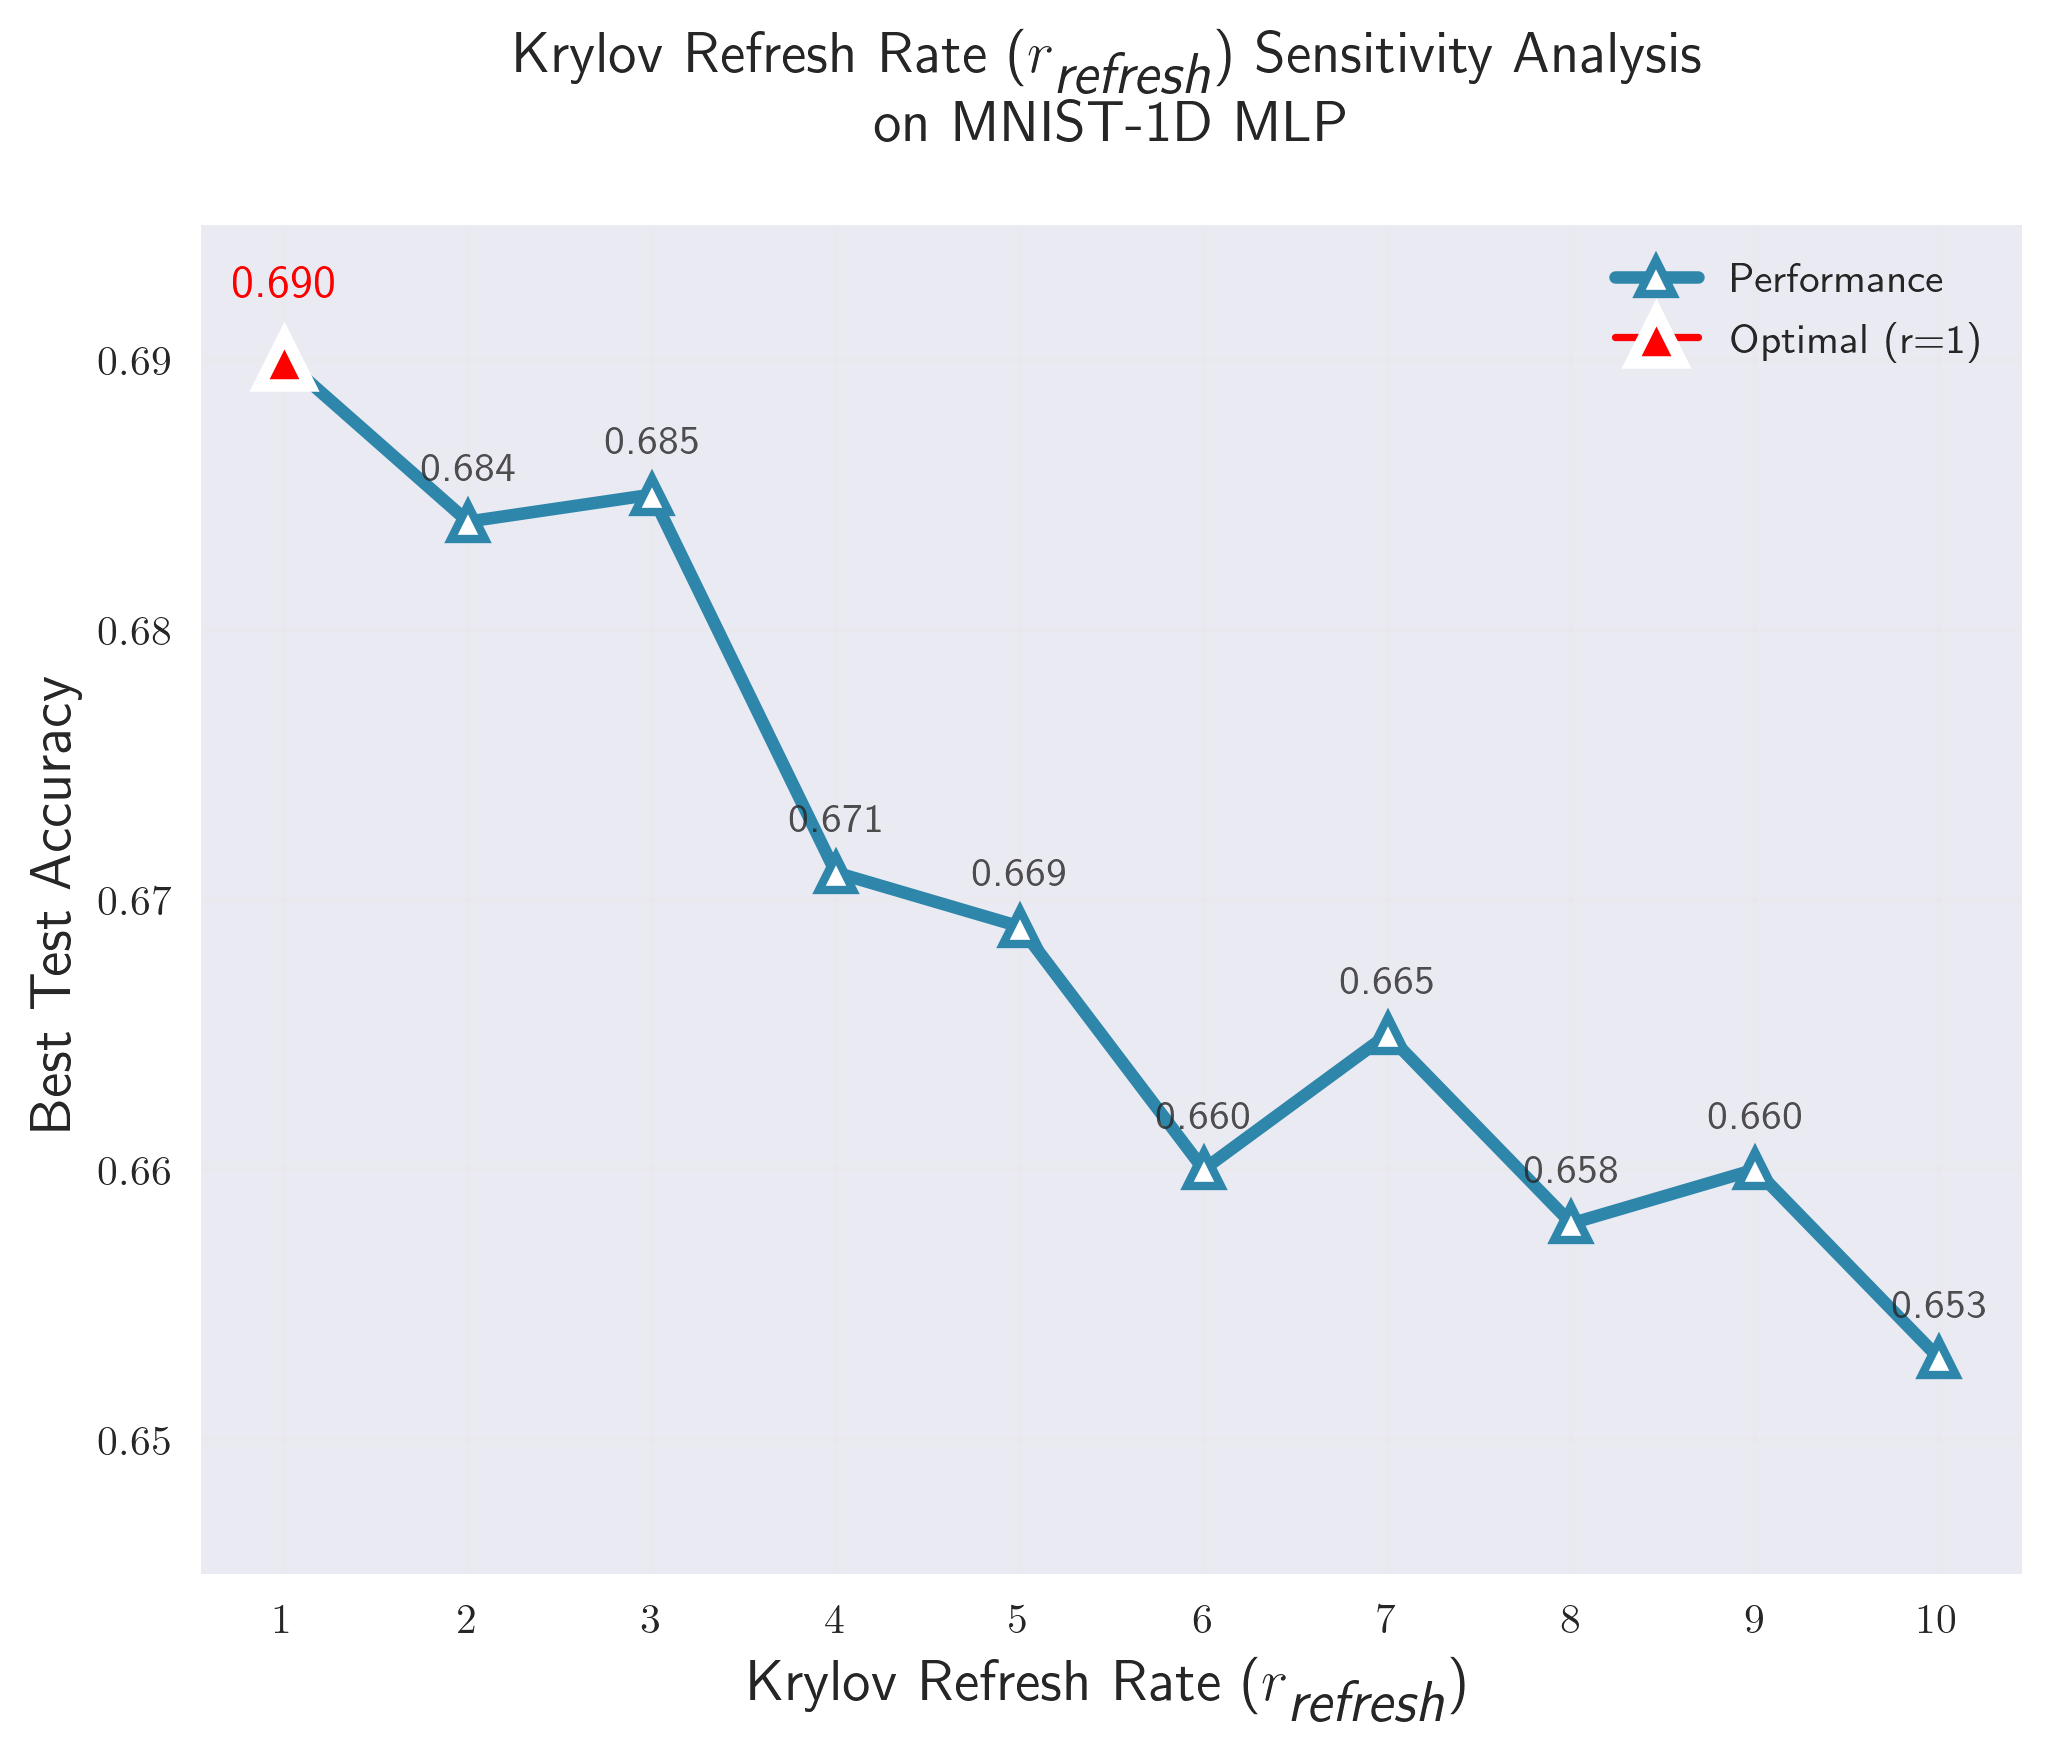
\includegraphics[width=\linewidth]{figures/5evals/sens_refresh.png}
        \caption{The sensitivity analysis of the krylov refresh rate $r_{\mathit{refresh}}$. on MNIST-1D MLP.}
        \label{fig:sens_r_refresh}
    \end{subfigure}
    \caption{Sensitivity analysis of KryBall on the MNIST-1D MLP task. We vary the Krylov dimension $M$, the maximum trust region radius $\Delta_{\mathit{max}}$, and the Krylov refresh rate $r_{\mathit{refresh}}$. The parameters are varied according to their hyperparameter ranges we defined in \cref{ssec:sensitivity_analysis}. The best performing point is marked in red.}
    \label{fig:sensitivity_analysis}
\end{figure}

\textbf{Krylov Subspace Size $(M)$}: We see that the Krylov subspace size $M$ is sensitive to the performance of KryBall. For low $M$, performance suffers since we are not able to approximate the Hessian well. As $M$ increases, we obtain good performance. However, as we continue to increase $M$ past a certain point (5), our performance plateaus. This is interesting, as usually a higher $M$ results in a better approximation. We suspect that for $M=5$ onwards, the dominant curvature information has already been captured. The new basis vectors that are generated are less relevant and do not add useful information, since we have already captured most of the curvature information previously. We present some further analysis about our approximation in \cref{sec:discussion_and_further_analysis}.
 
\textbf{Krylov Refresh Rate $(r_{\mathit{refresh}})$}: The Krylov refresh rate is best when $r_{\mathit{refresh}} = 1$. This is because when $r_{\mathit{refresh}} = 1$, we use compute the Krylov subspace at every single iteration and are always using the most information. As $r_{\mathit{refresh}}$ increases, we instead fall back to our approximation not at the current point in the optimisation landscape. This is fine if we our information is not too outdated, as is the case for $r_{\mathit{refresh}} = 2$ and $r_{\mathit{refresh}} = 3$. However, as $r_{\mathit{refresh}} \geq 4$ our information is outdated and thus our quadratic model approximation is no longer accurate. This results in KryBall performing worse. We choose $r_{\mathit{refresh}} = 3$ as our default value.

\section{Discussion and Further Analysis}
\label{sec:discussion_and_further_analysis}

In this section, we present critical questions about the results we have observed and the choices we have made in evaluating our algorithm. We then answer these questions with hypotheses, experiments and further analysis. 

\textbf{Why do we see late epoch instability but good early epoch performance?}

We saw in \cref{ssec:results_image_classification} that KryBall achieves good early epoch performance, but late epoch instability. We suspect this has to do with our quadratic approximation. In the early epochs, our quadratic model is accurate and a good approximation of the landscape. However, as training progresses, the landscape changes and we suspect that a quadratic model is less accurate. 

\cite{ma2022beyond} state that the loss landscape of neural networks is multiscale, and that the quadratic model is only a local approximation of the landscape. Specifically, they find that in a neighbourhood of the local minima, the loss mixes a continuum of scales and instead grows subquadratically. As dimensionality increases, they state that the loss landscape instead shows several separate scales. This means that our quadratic model is not accurate in the presence of local minima. Given that the loss landscape is multiscale, and more importantly subquadratic near the local minima, this means that a first-order approximation may be better. In \cref{fig:cifar10_cnn_acc} and \cref{fig:cifar10_resnet_acc}, it is plausible that the variance we see near the end of training is due to this. 

To illustrate this, we perform a small experiment. We take the MNIST-1D MLP model with SGD and at distinct points in the training process, we sample the loss landscape. This is done through an exhaustive line search over $\lambda \in [-2, 2]$. We then plot what the loss landscape is at the start and end of training. This empirically shows a slice of the loss landscape from the perspective of SGD. 

\begin{figure}[!t]
    \begin{subfigure}[b]{0.49\linewidth}
        \centering
        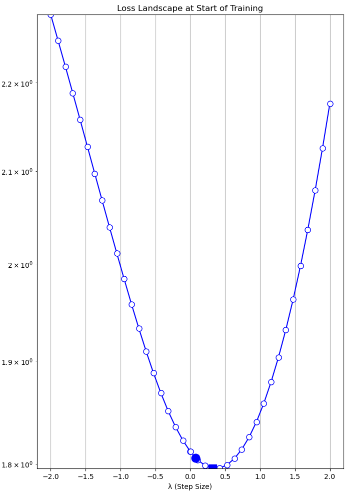
\includegraphics[width=\linewidth, height=0.4\textheight]{figures/5evals/ll_sgd_start.png}
        \caption{The loss landscape at the start of training (first epoch).}
        \label{fig:ll_sgd_start}
    \end{subfigure}
    \hfill
    \begin{subfigure}[b]{0.49\linewidth}
        \centering
        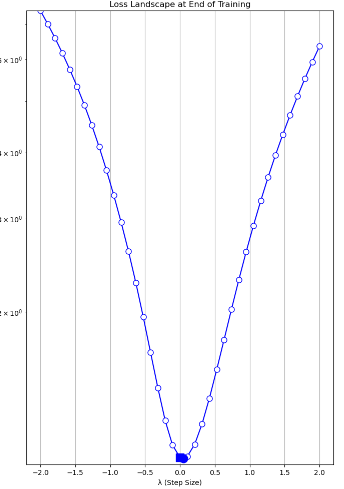
\includegraphics[width=\linewidth, height=0.4\textheight]{figures/5evals/ll_sgd_end.png}
        \caption{The loss landscape near the end of training (last epoch).}
        \label{fig:ll_sgd_end}
    \end{subfigure}
    \caption{The loss landscape of the MNIST-1D MLP model from the view of SGD.}
    \label{fig:ll_landscape}
\end{figure}

At the start of training, we see that the landscape is shaped exactly like a quadratic bowl in \cref{fig:ll_sgd_start}. However, near the end of training, that the landscape is approximately quadratic instead as seen in \cref{fig:ll_sgd_end}. It no longer is shaped exactly like a quadratic, but instead is stretched inwards. This agrees with \cite{ma2022beyond}, and it is plausible that this shape is similar to that of a subquadratic landscape.

\textbf{What is the effect of the activation function on our optimiser?}

All classification tasks in \cref{ssec:results_xor_classification} and \cref{ssec:results_image_classification} are evaluated with the Softplus activation function. Now, we examine the effect of the activation function on our optimiser. We evaluate the MNIST-1D MLP task with the following different activation functions using KryBall: ReLU, Softplus, Tanh and GeLU.

\begin{figure}[!t]
    \begin{subfigure}[b]{0.49\linewidth}
        \centering
        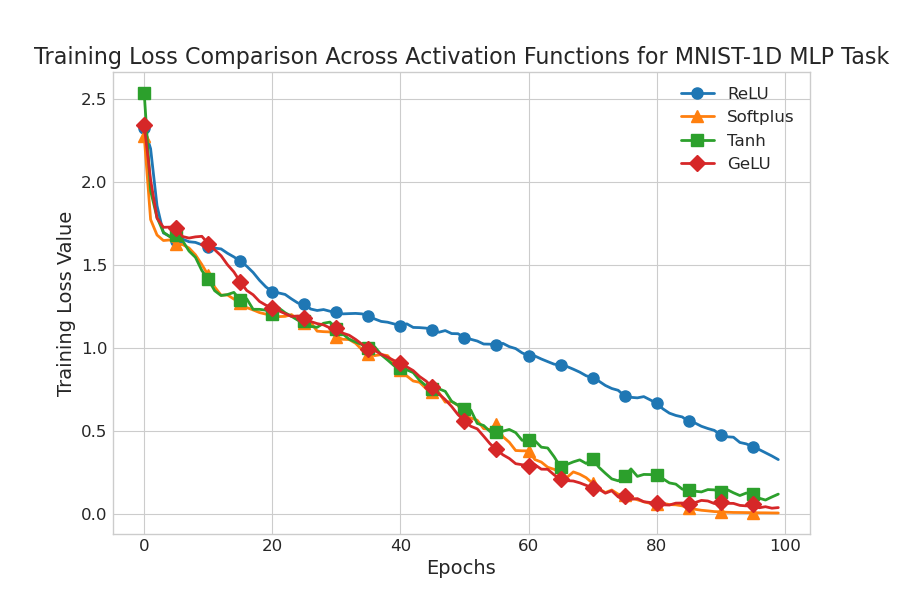
\includegraphics[width=\linewidth]{figures/5evals/mnist1d_activation_loss.png}
        \caption{Loss curves of the MNIST-1D MLP task with different activation functions using KryBall.}
        \label{fig:act_loss}
    \end{subfigure}
    \hfill
    \begin{subfigure}[b]{0.49\linewidth}
        \centering
        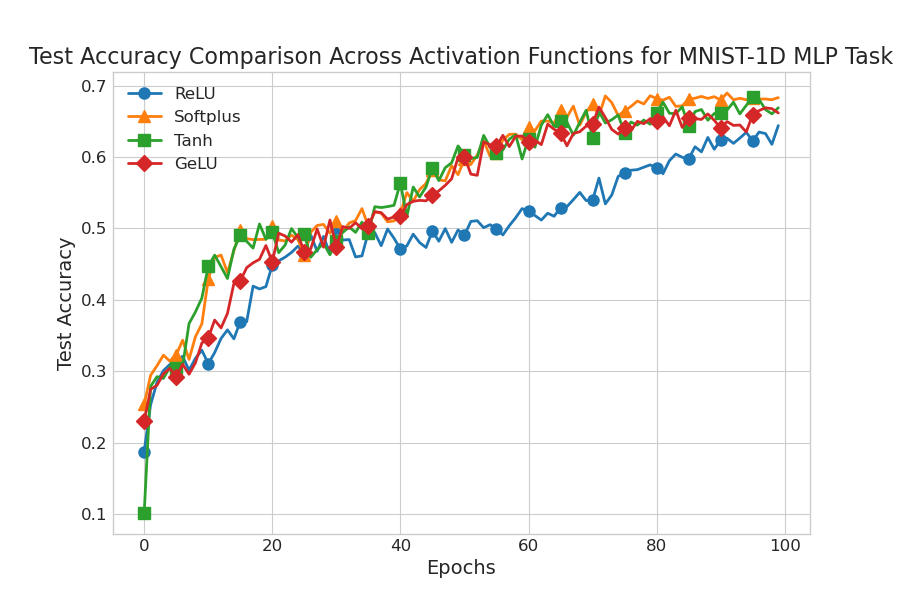
\includegraphics[width=\linewidth]{figures/5evals/mnist1d_activation_acc.png}
        \caption{Test accuracy of the MNIST-1D MLP task with different activation functions using KryBall.}
        \label{fig:act_acc}
    \end{subfigure}
    \caption{The loss curves and test accuracy of the MNIST-1D MLP task evaluated with KryBall and ReLU, Softplus, Tanh and GeLU activation functions.}
    \label{fig:act_results}
\end{figure}

In \cref{fig:act_results}, there is a stark distinction between the smooth activations and the non-smooth activation function ReLU. When using smooth activation functions, we reach close to training loss and our test accuracy is much better. However, the loss is much higher and our accuracy is lower when using ReLU. We have a good reason for this, which is that the quadratic approximation suffers in the presence of non-smooth activation functions. ReLU introduces non-differentiability at zero. This means that our quadratic model and trust-region framework, whose underlying assumptions are that we operate in smooth regions, is violated. Our method relise on meaningful HVPs for the approximation, but these are not well-defined at the transition points of ReLU units. This leads to poor curvature approximations.At this point, if we try to approximate the Hessian and the surrounding region using a quadratic model, we ultimately will not be able to. As such, it is better to use first-order methods that do not have these assumptions when using non-smooth activation functions. 

\textbf{Are our directions meaningful and distinct?}

\cite{tinysubspaces} show that gradients exhibit spurious alignment with the dominant eigenspace of the Hessian during training. Specifically, when the gradient appears to align with the top eigenspace, projecting it onto this subspace actually yields poor training progress \cite{tinysubspaces}. This finding suggests that our construction of distinct search directions is likely meaningful. Our method explicitly constructs directions from different sources. The SFN step, where we apply the $\abs{\cdot}$ function to the eigenvalues, alters the dominant subspace by ensuring positive definiteness. We hypothesis that this likely breaks the spurious alignment observed in standard training, making our dominant eigenspace directions genuinely useful rather than being correlated with the gradient. The strong empirical performance of KryBall on ill-conditioned problems, where eigenspace structure is critical. This supports the hypothesis that our multi-directional search strategy captures meaningful aspects of the optimisation landscape that individual directions cannot provide alone.

\textbf{How can we tell if our computed SFN step approximates the true SFN step?}

The crux of the Krylov subspace approach is to approximate the Hessian with a low-dimensional projected Hessian that lets us compute the SFN step. We now quantify how to analytically measure this approximation quality through the reconstruction error
\begin{align}
    ||r|| = ||z^* - \hat{z}||,
\end{align}
where $z^*$ is the true SFN direction and $\hat{z}$ is our Krylov approximation:
\begin{align}
    \hat{z} = \sum_{k=0}^{m-1} \alpha_k H^k \hat{g}.
\end{align}
Using the eigendecomposition $H = V \Lambda V^T$ and letting $c = V^T \hat{g}$, we can express both directions in terms of the eigenvalues. The true SFN direction becomes:
\begin{align}
    z^* = -V |\Lambda|^{-1} c,
\end{align}
while our Krylov approximation can be written as:
\begin{align}
    \hat{z} = V \left(\sum_{k=0}^{m-1} \alpha_k \Lambda^k\right) c.
\end{align}
We can then minimise the reconstruction error by formulating it as a linear system.
\begin{align}
    r &= z^* - \hat{z} = V(-|\Lambda|^{-1} - \sum_{k=0}^{m-1} \alpha_k \Lambda^k)c
\end{align}
We can minimise $r$ by setting the middle term to zero, in which we get,
\begin{align}
    &\Rightarrow -|\Lambda|^{-1} = \sum_{k=0}^{m-1} \alpha_k \Lambda^k \\
    &\Rightarrow -|\lambda_i|^{-1} = \sum_{k=0}^{m-1} \alpha_k \lambda_i^k \quad \text{for each eigenvalue } \lambda_i \\
    &\Rightarrow M\alpha = -1_r \quad \text{where } M_{i,k} = |\lambda_i| \lambda_i^k.
\end{align}
Solving this linear system for $\alpha$ and computing $||r||$ tells us how well our basis represents the ideal $|\Lambda|^{-1}$ operator. A small reconstruction error indicates that our limited Krylov subspace adequately spans the directions needed for an accurate SFN step. A large reconstruction error indicates that at the current point, our computed SFN step is not a good approximation of the true SFN step. Thus, we can use this to monitor the quality of our SFN step.

\section{Limitations and Improvements}
\label{sec:limitations}

While KryBall demonstrates promising performance across several optimisation tasks, our evaluation reveals important limitations. We now discuss these limitations and how to address them.

\subsection{Late-Epoch Instability}
\label{ssec:late_epoch_instability}

As demonstrated in our CIFAR-10 experiments, KryBall exhibits increased variance and instability in later training epochs. This occurs when the quadratic approximation becomes less accurate near local minima, where the loss landscape exhibits multiscale, subquadratic behaviour \citep{ma2022beyond}. We also saw empirical evidence of this when we sampled the optimiser trajectory in \cref{fig:ll_landscape}. One way to address this is to switch off the quadratic model and only use first-order information as we approach the local minima. This would likely require a heuristic where after a certain point in training, we switch off the quadratic model and only use either SGD or Adam. This is a hybrid approach, and we discuss this further in \cref{ssec:hybrid_approaches}.
    
\subsection{Dependence on Smooth Activation Functions}
\label{ssec:dependence_on_smooth_activation_functions}

A fundamental limitation of KryBall is that it requires smooth activation functions to operate effectively. Our analysis in \cref{fig:act_results} shows that non-smooth activation functions such as ReLU significantly degrade performance, as points of non-differentiability violate the underlying assumptions of the quadratic model. To address this, we require a way to approximate these points without using the quadratic model. Approximation by finite differences is one such method. This has been done by \cite{finite_diff} to approximate the Hessian cheaply, and has shown to be effective in CIFAR-10 classification tasks.

\subsection{Hyperparameter Sensitivity}
\label{ssec:hyperparameter_sensitivity}

Our sensitivity analysis reveals that KryBall is reasonably sensitive and dependent on the Krylov dimension $M$ and refresh rate $r_{\text{refresh}}$. We note that while our hyperparameters are not as sensitive as Adam and MSGD, they still require careful tuning, where suboptimal values can lead to poor performance as we saw in \cref{fig:sensitivity_analysis}. One way to address this could be to use adaptive schemes that automatically adjust $M$ and $r_{\text{refresh}}$. This has been done by \cite{henriques2019small}, who automatically rescale hyperparameters by using an objective change heuristic.

\subsection{Trust-Region Step Rejection}
\label{ssec:trust_region_step_rejection}

Our trust-region framework can reject optimisation steps when the quadratic model poorly predicts actual function behavior. While this provides stability, frequent step rejections can slow convergence compared to first-order methods that always accept their steps. This is particularly the case when the Hessian approximation degrades or is in highly non-quadratic regions. A good way to address this is to simply use the gradient or momentum as a fallback. Moreover, we can instead consider a hybrid approach where if our step is rejected, we proceed with a first-order optimiser such as Adam or MSGD.

\subsection{Computational Overhead}
\label{ssec:computational_overhead}

KryBall requires computing HVPs and constructing Krylov subspaces, introducing additional computational cost compared to first-order methods. While HVPs can be computed efficiently using automatic differentiation, the overall cost per iteration remains higher than gradient-only approaches. The key limitation here is that the main computational cost comes from the construction of the Krylov subspace, as our Krylov dimension $M$ is fixed throughout training. This overhead could be mitigated by adaptively reducing the Krylov dimension $M$ in regions where high-quality approximations are not critical, or by increasing the refresh rate $r_{\text{refresh}}$ when the landscape is relatively stable.

In this section, we presented the evaluations of our optimiser, KryBall, on a range of tasks. We evaluated KryBall's performance on ill-conditioned problems, simple binary classification, and more complex image classification tasks. We discussed KryBall's performance in comparison to the state-of-the-art optimisers Adam and MSGD. We then followed with a sensitivity analysis, a deeper discussion about key questions and finally the limitations of our method. We now move on to conclude this thesis.                    % evaluation
\chapter{Conclusion}
\label{chap:conclusion}

In this chapter, we summarise the main contributions of this thesis, discuss its implications and suggest future work directions.

\section{Summary}

In this thesis, we introduced KryBall, a novel second-order optimisation algorithm designed to address fundamental limitations in current optimisation methods for deep learning. We make a number of contributions that span both the practical and theoretical aspects of optimisation. 

For our theoretical contributions, we present the KryBall algorithm that combines the Saddle-Free-Newton method with a Krylov-subspace approach and integrates this within a trust-region framework. We connect the mathematical foundations of Krylov methods to practical optimisation performance, and address the issue of saddle point proliferation in high-dimensional spaces. We provide systematic analysis of loss landscape behaviour, problem conditioning, the effect of activation functions, and identify cases where our method excels and fails (such as when non-smooth activations are used). We also provide analytical tools for assessing the effectiveness of Krylov subspace approximations and demonstrate how to quantify the approximation error in our approach.

For the practical contributions, we present an implementation of Krylov subspace based Saddle-Free Newton methods integrated with a trust-region approach. We present the first $N$-dimensional subspace optimiser fully integrated with PyTorch, alongside an extensible testing suite. We also present our evaluations on ill-conditioned functions and classification tasks, where we demonstrate that KryBall is competitive with state-of-the-art methods, achieves rapid convergence on specific tasks, and is particularly well-suited to ill-conditioned problems.

\section{Future Work}
\label{sec:future_work}

While KryBall demonstrates promising performance across several optimisation tasks, our evaluation reveals several avenues for improvement and extension. The limitations identified in \cref{sec:limitations}, particularly around late-epoch instability, scalability, and dependence on smooth activation functions, point to promising research directions that can enhance our method. In this section, we outline key areas where future research could build upon our work. We discuss hybrid approaches, the need for theoretical rigour, improved model evaluations, support for non-smooth optimisation and computational efficiency.

\subsection{Hybrid Approaches}
\label{ssec:hybrid_approaches}

Our analysis in \cref{ssec:late_epoch_instability} revealed that KryBall exhibits late-epoch instability when the loss landscape transitions from quadratic to subquadratic behavior near convergence. A promising direction is developing hybrid optimisation schemes that dynamically switch between second-order and first-order methods based on local landscape. There are many approaches to do this. For example, we could run KryBall for the first $k$ iterations until we are no longer confident that our quadratic approximation is accurate, and then switch to MSGD or Adam. We could also run KryBall every $k$ iterations, interweaving the updates with MSGD or Adam through training. The second approach has already seen wide use. The Sophia optimiser, which we covered in \cref{chap:lit_review}, is an example of this approach, as it weaves its second order update with signSGD \citep{liu2023sophia}.

\subsection{Theoretical Rigour}
\label{sec:theoretical_rigour}

While we empirically evaluate KryBall and can adhere to the rapid convergence it exhibits in tasks such as ill-conditioned function optimisation and XOR classification, we currently lack strong theoretical guarantees. Future research should focus on establishing formal convergence rates and characterising the conditions in which approximation methods hold. For example, this involves developing theoretical frameworks that connect the reconstruction error analysis to actual convergence properties. We can further extend this by establishing error bounds on the approximation methods we use. This includes formalising theoretical upper and lower bounds, as well as introducing an expectation on the error introduced by the approximation methods. 

\subsection{Improved Model Evaluations}
\label{ssec:improved_model_evaluations}

Our evaluation focused primarily on small-scale problems, with ResNet-18 on CIFAR-10 representing the largest model tested. Future work should evaluate KryBall's scalability to contemporary large-scale applications such as transformer models, large convolutional networks, and other modern architectures. We also recommend expanding our evaluation suite to include more diverse tasks rather than just image classification. Examples of such tasks include natural language processing, such as language modelling on the Penn Treebank dataset \citep{penntreebank}, which involves predicting the next word in a sentence. Other tasks include 2D Neural Radiance Fields \citep{mildenhall2021nerf}. This involves predicting the radiance of a scene from a single image, and activation maximisation, which involves optimising an input image to maximise the activation of a specific neuron in a neural network \citep{activation_maximisation}.

\subsection{Non-Smooth Optimisation}
\label{ssec:non_smooth_optimisation_last}

Our analysis demonstrated that KryBall's performance degrades significantly with non-smooth activation functions like ReLU due to violations of the quadratic model's smoothness assumptions. Future research should explore specialised variants that handle non-differentiable points more effectively. This could be done by using finite difference approximations, as was discussed in \cref{sec:non_smooth_optimisation} or developing smoothed approximations of non-smooth activations, Another direction involves investigating how recent advances in non-smooth optimiation theory could be incorporated into Krylov-based methods to maintain second-order benefits while handling piecewise linear functions.

\subsection{Computational Efficiency}
\label{ssec:computational_efficiency}
We discussed the limitation of having computational overhead in \cref{ssec:computational_overhead}. As such, future work could focus on exploring ways to reduce the computation overhead associated with second-order methods. First, developing more efficient Arnoldi iteration implementations that exploit sparsity patterns or low-rank structure could reduce the cost of subspace construction. Secondly, we can investigate adaptive schemes that dynamically adjust hyperparameters depending on the current point in the optimisation landscape. This ensures that parameters like the Krylov dimension $M$ and the Krylov refresh rate $r_\textit{refresh}$ are only updated when necessary. Thirdly, we explore research into creating parallelisable and distributed computing algorithms for common matrix operations, such as matrix inversion and eigendecomposition. These directions could significantly improve practical performance, and in combination with researching theoretical guarantees as stated in \cref{sec:theoretical_rigour}, we could ensure that second-order methods are more widely adaptable.

\section{Concluding Thoughts}
\label{sec:concluding_thoughts}

Optimisation in deep learning is a challenging problem, but it is fundamental for advancing the state-of-the-art. Optimisation has led to the development of powerful models, techniques and novel innovations. The work presented in this thesis is a step towards more efficient optimisation. We present KryBall, our second-order optimisation algorithm that combines the advantages of first and second-order methods by using Krylov subspaces, the Saddle-Free-Newton, and a trust-region framework. We thus take a step towards the goal of efficiently navigating the optimisation landscape, and improving the performance of integral machine learning models and tasks in today's world.                    % conclusion

% \appendix
% \chapter{Appendix: Explanation on Appendices}\label{chap:appendix1}

You may use appendices to provide additional information that is in principle relevant to your work, though you don't want \emph{every reader} to look at the entire material, but only those interested.

There are many cases where an appendix may make sense. For example:
\begin{itemize}
  \item You developed various variants of some algorithm, but you only describe one of them in the main body, since the different variants are not that different.
  \item You may have conducted an extensive empirical analysis, yet you don't want to provide \emph{all} results. So you focus on the most relevant results in the main body of your work to get the message across. Yet you present the remaining and complete results here for the more interested reader.
  \item You developed a model of some sort. In your work, you explained an excerpt of the model. You also used mathematical syntax for this. Here, you can (if you wish) provide the actual model as you provided it in probably some textfile. Note that you don't have to do this, as artifacts can be submitted separately. Consult your supervisor in such a case.
  \item You could also provide a list of figures and/or list of tables in here (via the commands \verb!\listoffigures! and \verb!\listoftables!, respectively). Do this only if you think that this is beneficial for your work. If you want to include it, you can of course also provide it right after the table of contents. You might want to make this dependent on how many people you think are interested in this.
\end{itemize}
                    % appendix 1
% \chapter{Appendix: Explanation on Page Borders}\label{chap:appendix2}

What you find here is an explanation of why the border width keeps flipping from left to right -- which you might have spotted and wondered why that's the case.

Firstly, that is \emph{intended} and thus correct, so there is no reason to worry about this. The reason is that this document is configured as a two-sided book, which means:
\begin{compactitem}
  \item We assume the document will be printed out,
  \item that this will be done in a two-sided mode (i.e., the document will be printed on both sides of each page), and
  \item that the bookbinding will be in the middle, just like in every book.
\end{compactitem}

When you open the book, there are three borders of equal size~$n$. This however requires that even pages have a border of $n$ on their left and $\frac{n}{2}$ on their right, and odd pages have a border of $\frac{n}{2}$ on their left and $n$ on their right. This is illustrated in Figure~\ref{fig:pageBorders}.

\begin{figure}[h]
  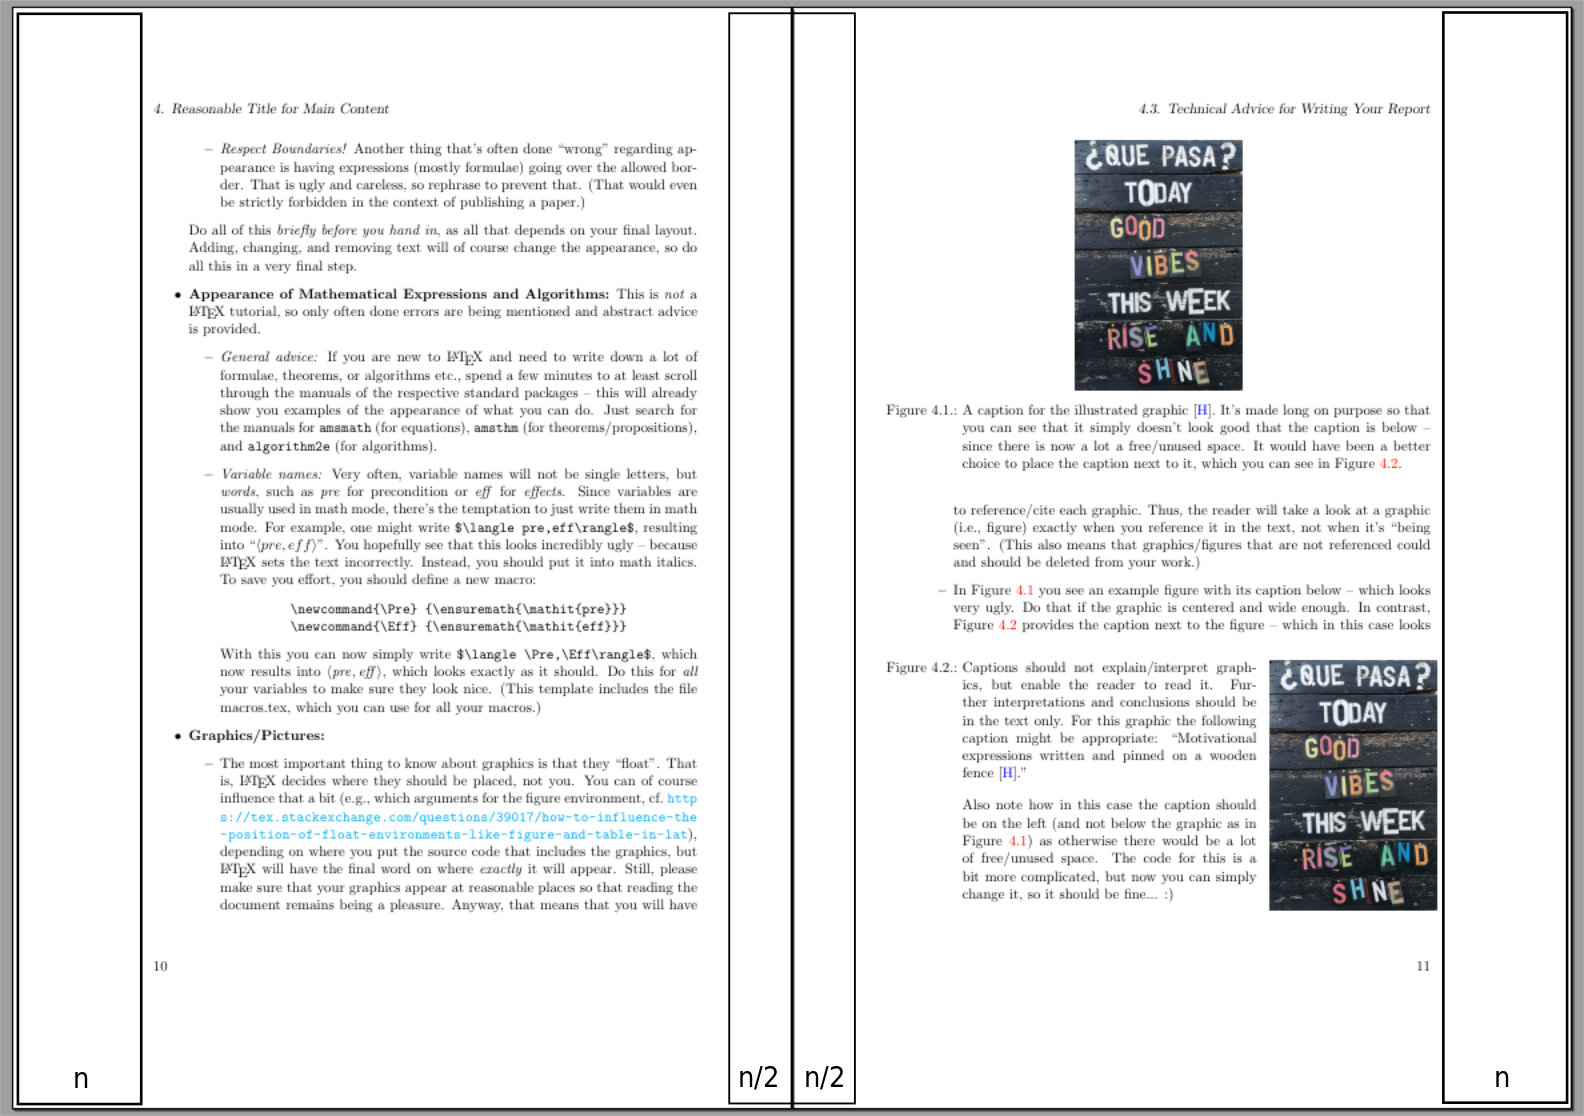
\includegraphics[width=.55\textwidth]{figures/borders--annotated}
  \caption{Illustration showing why page borders flip.\label{fig:pageBorders}}
\end{figure}%

                    % appendix 2


% literature
\bibliographystyle{anuthesis} % or plainnat or whatever
\cleardoublepage\phantomsection
% see https://tex.stackexchange.com/questions/60556/link-to-bibliography-in-the-toc-fails
\bibliography{bib}
\end{document}
